Top quark pair production with at least one \tauhadvis candidate
originating from a misidentified quark- or gluon-initiated jet is the
second largest background in the \hadhad channel. A large fraction of
\SI{85}{\percent} of this background stems from semi-leptonic decay
modes of \ttbar where the selected \tauhadvis candidates consist of
one true- and one \faketauhadvis. The fraction of \ttbarFakes events
where both candidates are \faketauhadvis is about \SI{15}{\percent}
and therefore comparatively small. The \ttbarFakes background is
estimated using simulation after applying data-driven corrections in
the form of \faketauhadvis scale factors (SFs) measured in a control
region enriched in \ttbar events. The SFs correct the \jettotauhadvis
misidentification efficiencies predicted by simulation which are, in
general, not centrally calibrated by the ATLAS collaboration due to
their process dependency.

Before proceeding with the description of the method, differences
between \faketauhadvis backgrounds from multi-jet and \ttbar are
highlighted that motivate the use of different background estimation
techniques:
\begin{itemize}

\item The majority of \ttbarFakes background events consist of only
  one \faketauhadvis while in multi-jet events both candidates are
  \faketauhadvis.

\item The probability of quark- or gluon-initiated jets reconstructed
  as \tauhadvis to pass \tauid, the so-called fake rate, depends on
  the type of parton that initiated the jet. \Faketauhadvis from
  \ttbar predominately originate from jets produced in hadronic decays
  of $W$~bosons which have larger fake rates than jets originating
  from gluons.

\item In the \hadhad channel, no suitable \ttbarFakes control region
  can be defined that allows to separate \faketauhadvis backgrounds
  from \ttbar and multi-jet while maintaining sufficient statistical
  precision for background estimation. This necessitates defining a
  control region in $\ell + \tauhadvis$ ($\ell = e, \mu$) final states
  where the multi-jet contribution is negligible.

\end{itemize}
The main disadvantage of separately estimating the \faketauhadvis
background from \ttbar and multi-jet is the inflation of systematic
uncertainties on the total \faketauhadvis background compared to a
combined approach.\footnote{A concrete example is the combined fake
  factor method employed in the \lephad channel that is discussed
  in~\Cref{sec:bkg_lephad_combined_ff}.} However, these inflated
uncertainties have little effect of the signal sensitivity. This is
because the targeted signal processes have distinct kinematic
properties that differentiate them from \faketauhadvis backgrounds,
and the search being limited by statistical uncertainties as opposed
to systematic ones.


\subsubsection{Control Region Definition}

% The measurement is performed in a control region by comparing the
% prediction of \ttbarFakes from simulation with observed data. The
% control region should have high \ttbar purity with a measurable
% contribution of \ttbarFakes and exactly one \tauhadvis candidate to
% isolate the effect of differences in misidentification efficiencies
% between simulation and data. Corrections are defined as
% multiplicative scale factors (SF) applied to \faketauhadvis passing
% \tauid in simulation and measured as a functions of \faketauhadvis
% properties using a maximum likelihood fit of a discriminating
% distribution in the control region.  In the \hadhad signal region,
% the measured scale factors are applied to simulated \ttbarFakes
% events to obtain the background prediction and the associated
% uncertainties.

The control region for the scale factor measurement (SF-CR) targets
final states with an electron or muon and a \tauhadvis candidate. The
region definition is based on the selections applied in the \lephad
channels where a similar control region is used for \faketauhadvis
background estimation. Minor changes are applied to its definition to
ensure consistency with the signal region selection of the \hadhad
channel. The most important selection criteria and differences are
briefly summarised:
\begin{itemize}

\item The \tauhadvis selection is adapted to follow the selection of
  the \hadhad channel more closely by selecting candidates with
  $\pT > \SI{25}{\GeV}$ and $|\eta| < \num{2.5}$ (instead of
  $\pT > \SI{20}{\GeV}$ and $|\eta| < \num{2.3}$ in the \lephad
  channels).

\item All events are required to have exactly one \tauhadvis passing
  identification, exactly one electron or one muon passing their
  respective isolation and identification criteria, and exactly two
  \btagged jets. In addition, only events selected by single-lepton
  triggers are considered.

\item The electron or muon and the \tauhadvis candidate are required
  to be reconstructed with electric charges of opposite sign. This
  requirement ensures that the charge correlations between light
  lepton and \faketauhadvis from semi-leptonic decays of \ttbar are
  similar to the correlation between \tauhadvis candidates from
  \ttbarFakes in the \hadhad signal region for cases where only one
  candidate is a \faketauhadvis. The effect of charge correlation on
  \ttbarFakes estimation was previously studied in Ref.~\cite{bokan}.

\item Orthogonality between the SF-CR and the signal region of the
  \lephad SLT channel is ensured by requiring $\mBB > \SI{150}{\GeV}$.

\end{itemize}

% \footnote{Leptons $\ell$ and true \tauhadvis are have high
% probability to be reconstructed with the correct electric charge in
% the SF-CR. In \ttbar the \faketauhadvis candidate is more likely to
% have opposite-sign electric charge . As a result, in the same-sign
% region the quark/gluon composition of jets is likely different which
% also affects the fake rates.}.

The control region selects \ttbar with high purity of
\SI{94}{\percent} prior to the fit. About \SI{66}{\percent} of
selected events are from di-leptonic decay channels of \ttbar yielding
$\ell + \tauhad$ final states, where $\ell$ is either an electron or
muon. The production of \ttbar events with \tauhadvis originating from
quark- or gluon-initiated jets, which is the process of interest for
this measurement, constitutes \SI{28}{\percent} of all selected
events. Minor backgrounds in this region are single top
(\SI{4}{\percent}) and $\Vjets$ production (\SI{2}{\percent}). The
contribution of \multijet background is negligible based on studies
performed as part of the \faketauhadvis estimation in the \lephad
channel. The distribution of transverse momenta and pseudorapidity of
\tauhadvis candidates in the SF-CR prior to the fit is shown
in~\Cref{fig:ttbarSF_prefit_pt}.

\begin{figure}[htbp]
  \centering

  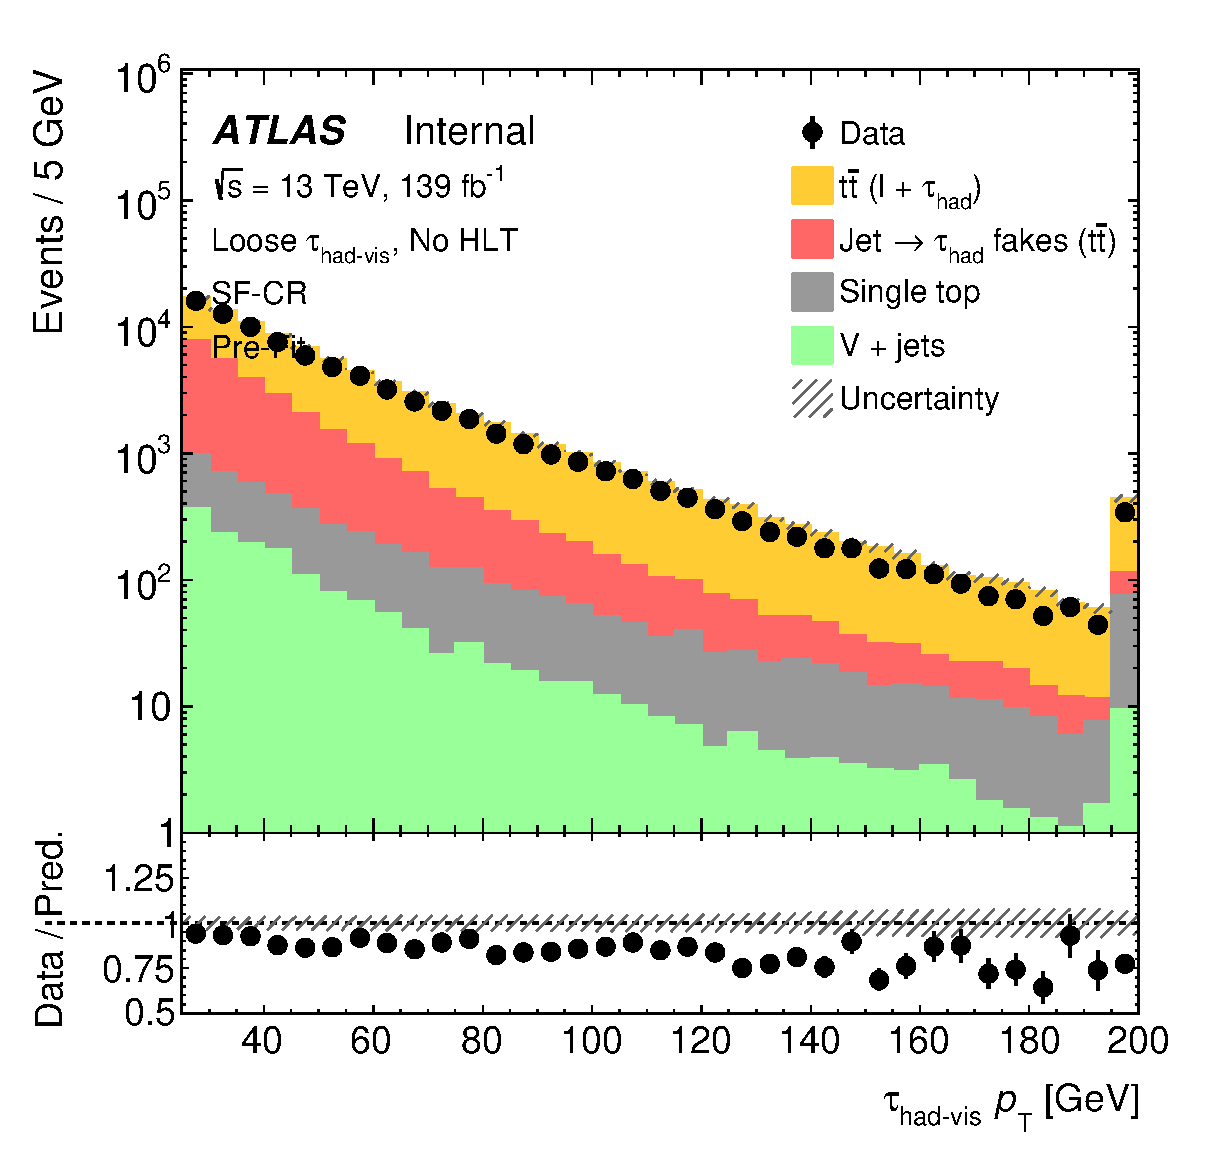
\includegraphics[width=0.49\textwidth]{ttbarSF/prefit_sfcr/PTVR}%
  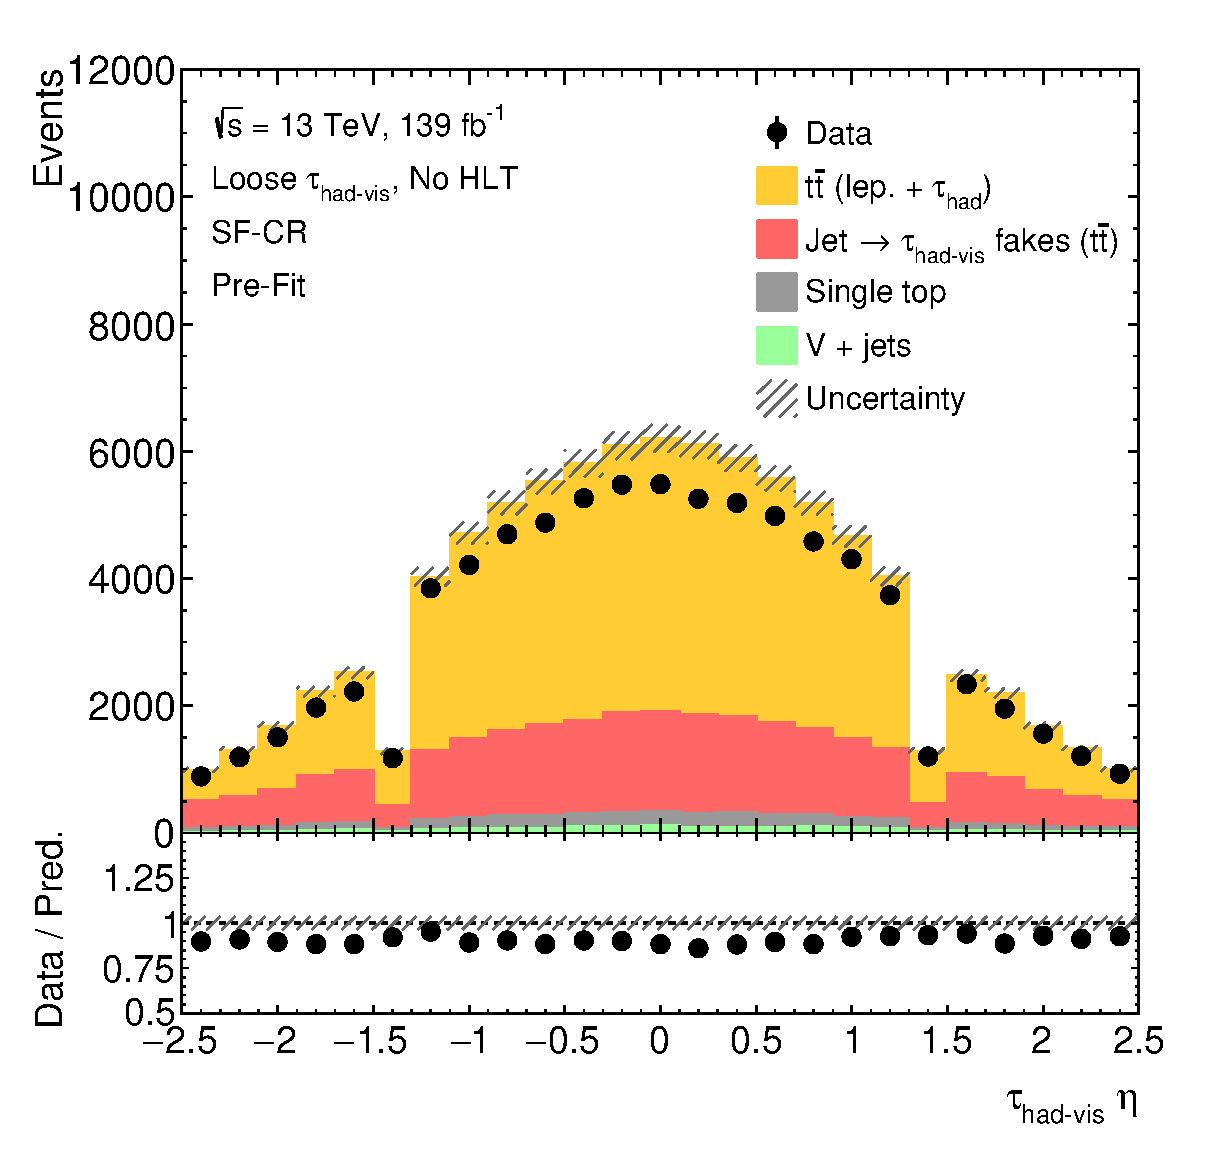
\includegraphics[width=0.49\textwidth]{ttbarSF/prefit_sfcr/ETAVR}

  \caption{Distribution of \tauhadvis \pT and $\eta$ in the scale
    factor control region prior to the maximum likelihood fit. Events
    with \tauhadvis \pT larger than \SI{200}{\GeV} are merged into the
    last bin. The uncertainty contains all statistical and systematic
    uncertainties except for normalisation uncertainties on \ttbar
    arising from its modelling in simulation. Modelling uncertainties
    affecting the shape of the distributions are included.}%
  \label{fig:ttbarSF_prefit_pt}
\end{figure}

\Jettotauhadvis misidentification efficiencies depend on the
identification requirements applied to \tauhadvis candidates. In this
search, all \tauhadvis candidates from the offline reconstruction have
to pass the loose RNN \tauid working point. In addition, events in the
\hadhad channel are selected using \tauhadvis triggers which apply
their own isolation and identification requirements to trigger-level
\tauhadvis in order to reduce the trigger-rates at various stages of
the ATLAS trigger system. Calorimeter-based isolation cuts are applied
to \tauhadvis candidates at the Level-1 trigger, while at the HLT more
sophisticated \tauid algorithms, similar to their counterparts from
the offline reconstruction, are used. Some differences in the
selection applied at trigger-level and during offline event
reconstruction are expected due to limitations in detector read-out
and time budget in the trigger
system. % New developments introduced into offline \tauhadvis
% reconstruction during Run~2 of the LHC, such as the RNN \tauid, can
% lead to additional differences as they cannot be applied retroactively
% to past data-taking periods.

The effect of the two-stage selection of \tauhadvis based on
identification criteria, first at trigger-level and then during
offline event reconstruction, is taken into account when measuring
corrections to the \jettotauhadvis misidentification efficiencies. All
combinations of \tauhadvis identification requirements relevant for
the signal region selection of the \hadhad channel are considered. The
offline \tauhadvis identification is the same for all events, however,
the trigger-level requirements vary. In events selected by
single-\tauhadvis triggers one \tauhadvis candidate has to pass the
trigger-level selection while no additional requirements are placed on
the other \tauhadvis candidate. For di-\tauhadvis triggers both
candidates have to fulfil the trigger requirements. The scale factor
measurement for \tauhadvis candidates without trigger requirements can
proceed using SF-CR events directly as single-electron and single-muon
triggers are used to select events.

The trigger-level \tauhadvis selection can be emulated by requiring
that events in the SF-CR also pass an appropriately chosen
single-\tauhadvis trigger. Moreover, \tauhadvis candidates from the
offline event reconstruction are required to be geometrically matched
($\Delta R < 0.2$) to a reconstructed and identified \tauhadvis
candidate at the HLT. The \tauhadvis triggers used for this procedure
are chosen to reflect the trigger selection of the \hadhad channel,
previously described in \Cref{sec:exp_trigger}.

The lowest transverse momentum threshold on \tauhadvis at the HLT
relevant to this search is $\pTHLT > \SI{25}{\GeV}$. This threshold
applies to the sub-leading \tauhadvis candidate in events selected by
di-\tauhadvis triggers. Single-\tauhadvis triggers with a
\SI{25}{\GeV} transverse momentum threshold are only available with
the application of a prescale\footnote{A trigger with a prescale value
  of $n$ accepts events satisfying the trigger conditions with a
  probability of $1 / n$ \cite{TRIG-2019-04}.} to limit their
trigger-rates. However, all events entering the SF-CR were already
recorded using single lepton triggers, allowing to re-run the trigger
algorithms such that the trigger decisions of the single-\tauhadvis
triggers can be \textit{resurrected} without applying the
prescale. The single-\tauhadvis triggers relevant to this search are
listed in the following:%
\begin{itemize}
\item \verb|HLT_tau25_medium1_tracktwo|: Trigger chain used for
  data-taking from 2015 to 2017. Resurrected trigger decisions are
  available for the entirety of the Run~2 dataset corresponding to
  \SI{139}{\ifb} of integrated luminosity.

\item \verb|HLT_tau25_medium1_tracktwoEF|: Primary trigger chain used
  for data-taking in 2018. Resurrected trigger decisions are only
  available for runs in 2018 corresponding to an integrated luminosity
  of \SI{58}{\ifb}.

\item \verb|HLT_tau25_mediumRNN_tracktwoMVA|: Supplementary trigger
  chain introduced during data-taking in 2018 (from
  period~K). Resurrected trigger decisions are available for a partial
  2018 dataset corresponding to \SI{37}{\ifb} of integrated
  luminosity. This trigger chain is to be used in conjunction with the
  previous item. Hereafter, when referring to
  \verb|HLT_tau25_mediumRNN_tracktwoMVA| a ``logical or'' with
  \verb|HLT_tau25_medium1_tracktwoEF| is implied.

\end{itemize}

Four combinations of \tauhadvis selections need to be considered when
measuring corrections to the \jettotauhadvis misidentification
efficiencies in \ttbar. When no additional trigger requirements are
applied the scale factors can be measured in the SF-CR directly. Three
subregions of the SF-CR, each corresponding to one of the trigger
chains, are defined for cases where requirements are imposed on
\tauhadvis at trigger-level. Events entering these regions are
required to be selected by the respective resurrected trigger and the
reconstructed \tauhadvis candidate has to be geometrically matched to
an identified \tauhadvis candidate at the HLT. Separate scale factor
measurements are performed in these regions.

% These are defined by ensuring that the resurrected triggers select the
% event and that the reconstructed \tauhadvis candidate is geometrically
% matched to the \tauhadvis candidate at the HLT.


\subsubsection{Measurement and Fit Model}

The \jettotauhadvis misidentification efficiencies strongly depend on
the charged particle multiplicity and visible transverse momentum of
reconstructed \tauhadvis candidates. This can be also reflected in
corrections to the \jettotauhadvis misidentification efficiency in
simulation. Therefore, the scale factor measurement is performed in
bins of the reconstructed \tauhadvis decay mode (1- or 3-prong) and
\tauhadvis~\pT. This is achieved by performing the scale factor
measurement simultaneously in several disjoint subregions defined as:
\begin{itemize}

\item 1-prong \tauhadvis with $\pT / \si{\GeV}$: $[25, 30)$, $[30, 35)$,
  $[35, 40)$, $[40, 45)$, $[45, 55)$, $[55, 70)$, $[70, \infty)$.

\item 3-prong \tauhadvis with $\pT / \si{\GeV}$: $[25, 30)$, $[30, 40)$,
  $[40, 50)$, $[50, 70)$, $[70, \infty)$.

\end{itemize}
The regions are chosen such that their size allows for a determination
of the corrections with limited impact of statistical uncertainties
while allowing to extract potential \pT dependencies of the correction
factors. In cases where trigger-matching is applied, the \tauhadvis
\pT interval from 25 to \SI{30}{\GeV} is omitted due to the triggers
not being fully efficient in this region. This is analogous to the
selection applied for the \hadhad signal region. Exemplary summaries
of event yields in the measurement regions are shown
in~\Cref{fig:ttbarsf_region_summary_prefit}.

\begin{figure}[htbp]
  \centering

  \begin{subfigure}[t]{.485\textwidth}
    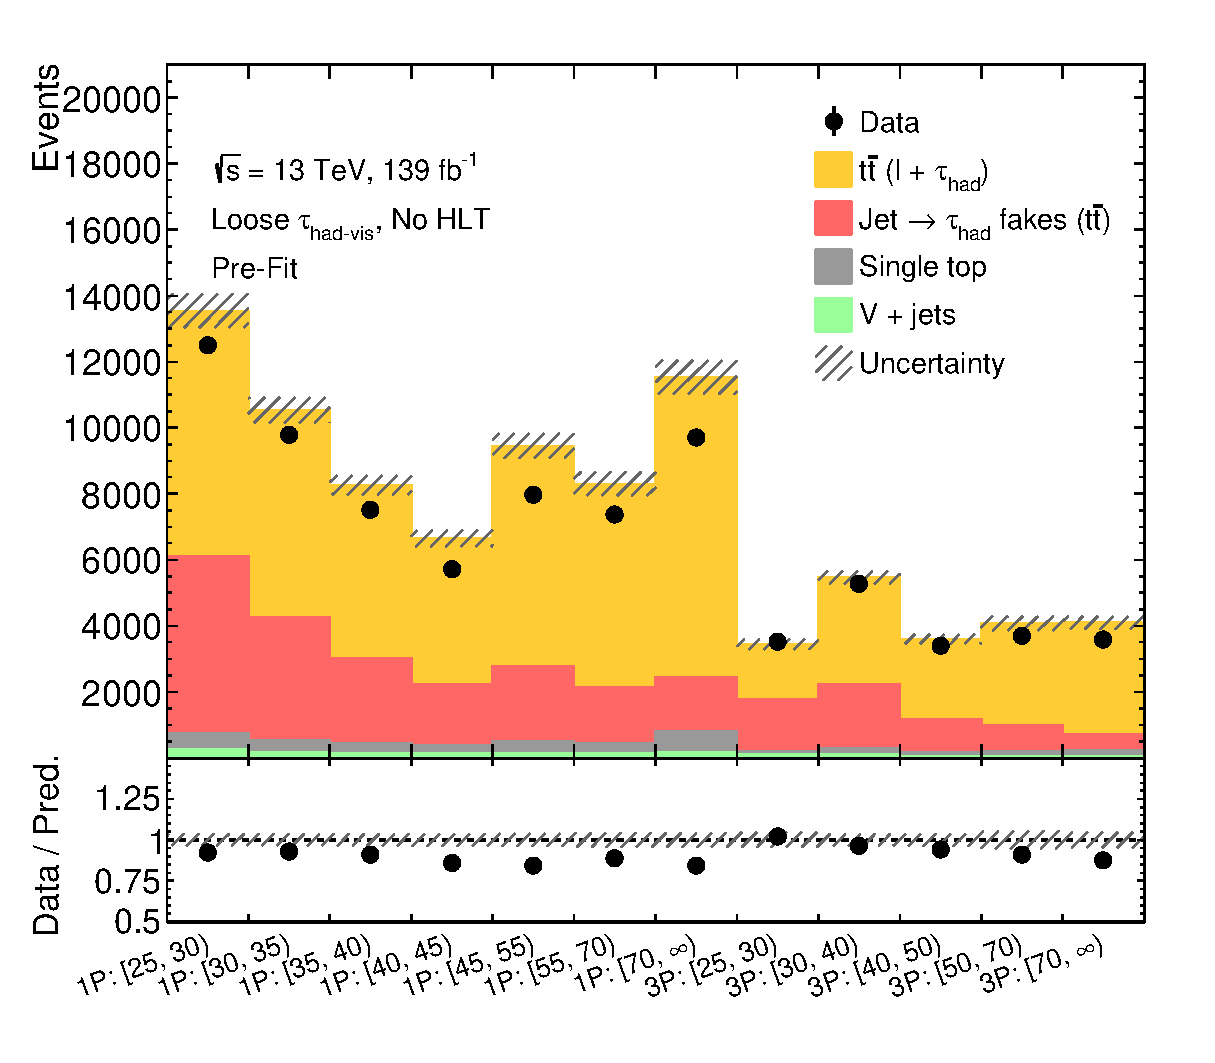
\includegraphics[width=\textwidth]{ttbarSF/Summary_offl}
    \caption{Top control region for events passing the loose working
      point of the offline \tauid without application of
      trigger-matching.}
  \end{subfigure}\hfill%
  \begin{subfigure}[t]{.485\textwidth}
    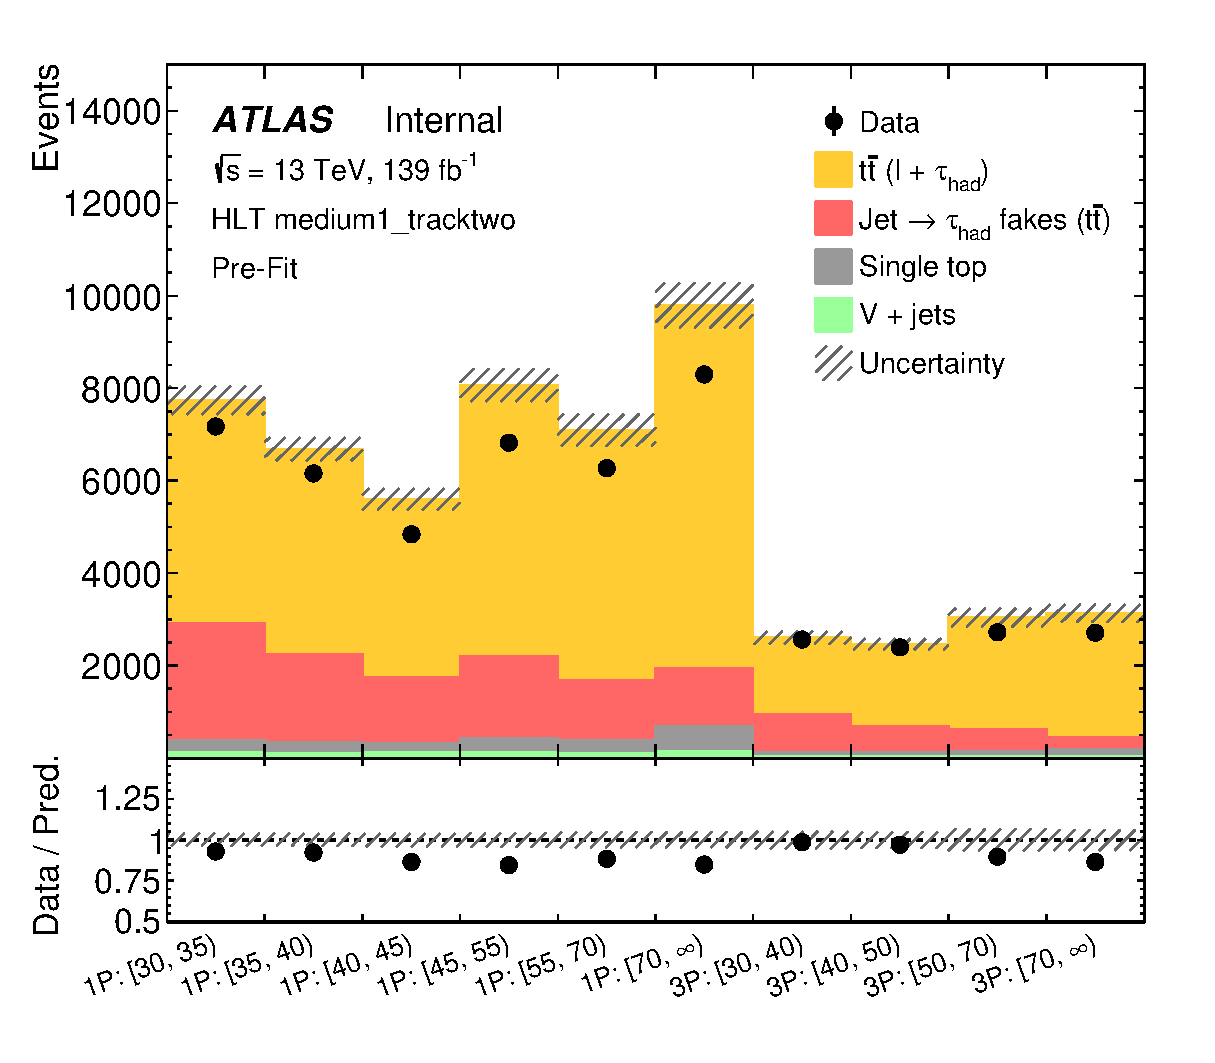
\includegraphics[width=\textwidth]{ttbarSF/Summary_tau25}
    \caption{Top control region for events passing the resurrected
      \texttt{HLT\_tau25\_medium1\_tracktwo} trigger,
      trigger-matching, and the loose working point of the offline
      \tauid.}
  \end{subfigure}

  \caption{Summary of event yields in regions used for determination
    of the \jettotauhadvis misidentification efficiency
    corrections. The $x$-axis shows the measurement regions separated
    by the reconstructed decay mode into either 1-prong (1P) and
    3-prong (3P) \tauhadvis and the \tauhadvis $\pT /\si{\GeV}$ bin
    interval. The pre-fit background model is shown.}%
  \label{fig:ttbarsf_region_summary_prefit}
\end{figure}

The top control region has large contributions of \ttbar with a
di-lepton final state where the \tauhadvis candidate originates from a
\tauhad decay. This contribution is not sensitive to the
\jettotauhadvis misidentification efficiency but has to be estimated
when extracting correction factors. To distinguish between di-leptonic
\ttbar with true \tauhadvis and semi-leptonic \ttbar with
\faketauhadvis, an estimate of the transverse mass between the lepton
$\ell$ and \pTmissAbs given by
\begin{align*}
  \mTW = \sqrt{2 | \myvec{p}_{\text{T}}^{\ell} | | \pTmiss | \left( 1 - \cos \Delta\phi \right)}
\end{align*}
is used, where $\Delta \phi$ is the angle between the lepton
transverse momentum~$\myvec{p}_{\text{T}}^{\ell}$ and the missing
transverse momentum~\pTmiss.

The distribution of \mTW in the SF-CR is shown
in~\Cref{fig:ttbarsf_mtw_pdf} separately for di- and semi-leptonic
decay modes of \ttbar. For semi-leptonic \ttbar, the primary source of
\faketauhadvis, the event rate diminishes quickly for transverse
masses beyond the mass of the \PW boson. In contrast, di-leptonic
\ttbar final states show a comparatively heavy tail towards large
values of \mTW due to the presence of an additional neutrino. The \mTW
distribution of semi-leptonic \ttbar remains stable with respect to
changes in the considered momentum range for the reconstructed
\tauhadvis candidate. This is not the case for the di-lepton
contribution where the tail towards high \mTW is further enhanced with
increasing \pT of the \tauhadvis candidate\todo{Show?}.

% The primary source of events containing a \faketauhadvis is
% semi-leptonic \ttbar with an electron or muon and additional jets from
% the hadronic decay of a \PW boson. This contribution features a quick
% reduction in event rate for transverse masses beyond the mass of the
% \PW boson.

\begin{figure}[htbp]
  \centering

  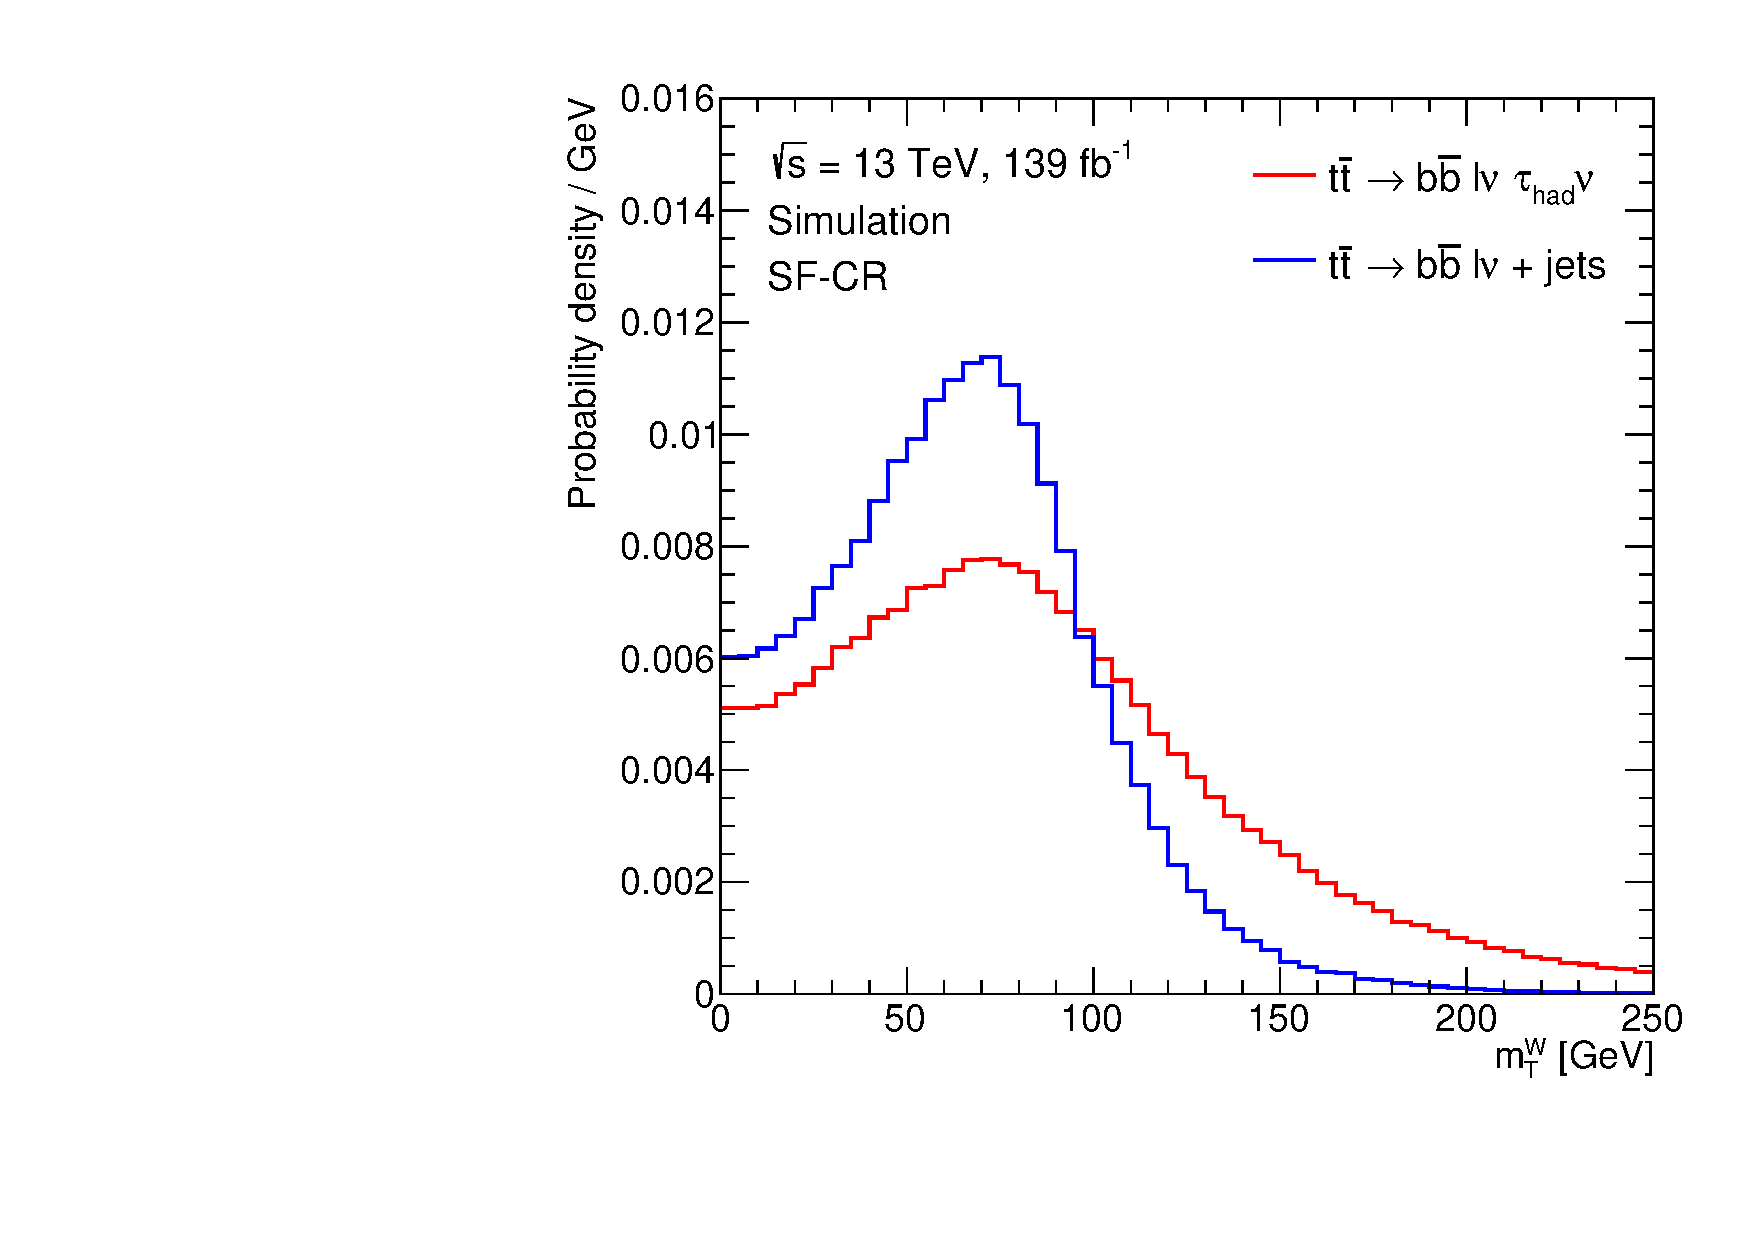
\includegraphics[width=0.45\textwidth]{ttbarSF/mtw_pdf}

  \caption{Distribution of the transverse mass between the light
    lepton and \pTmiss in simulated \ttbar events entering the
    SF-CR. Events are shown inclusive in the \tauhadvis transverse
    momentum and decay mode without requirements on the
    trigger-matching.}%
  \label{fig:ttbarsf_mtw_pdf}

  \todo[inline]{Y-axis should be per GeV.}
\end{figure}

All subregions of the SF-CR defined by the reconstructed \tauhadvis
decay mode and \pT are included in a simultaneous fit of the scale
factors. When performing the measurement for events after the
\tauhadvis trigger selection, events are required to pass the
corresponding resurrected trigger and trigger-matching. Each subregion
enters the fit with five \mTW bins to distinguish between \ttbar with
\faketauhadvis and \tauhadvis from hadronic \taulepton
decays. In~\Cref{fig:ttbarsf_mtw_examples_prefit} the \mTW
distribution is shown prior to the fit for two exemplary regions after
the trigger-matching requirement.

% The regions entering the fit are determined by the charged particle
% multiplicity of the reconstructed \tauhadvis candidate and the
% reconstructed \tauhadvis \pT. For the measurement after HLT \tauhadvis
% identification the events entering the fit are also required to pass
% trigger matching to the resurrected trigger of interest.

\begin{figure}[htbp]
  \centering

  \begin{subfigure}{.485\textwidth}
    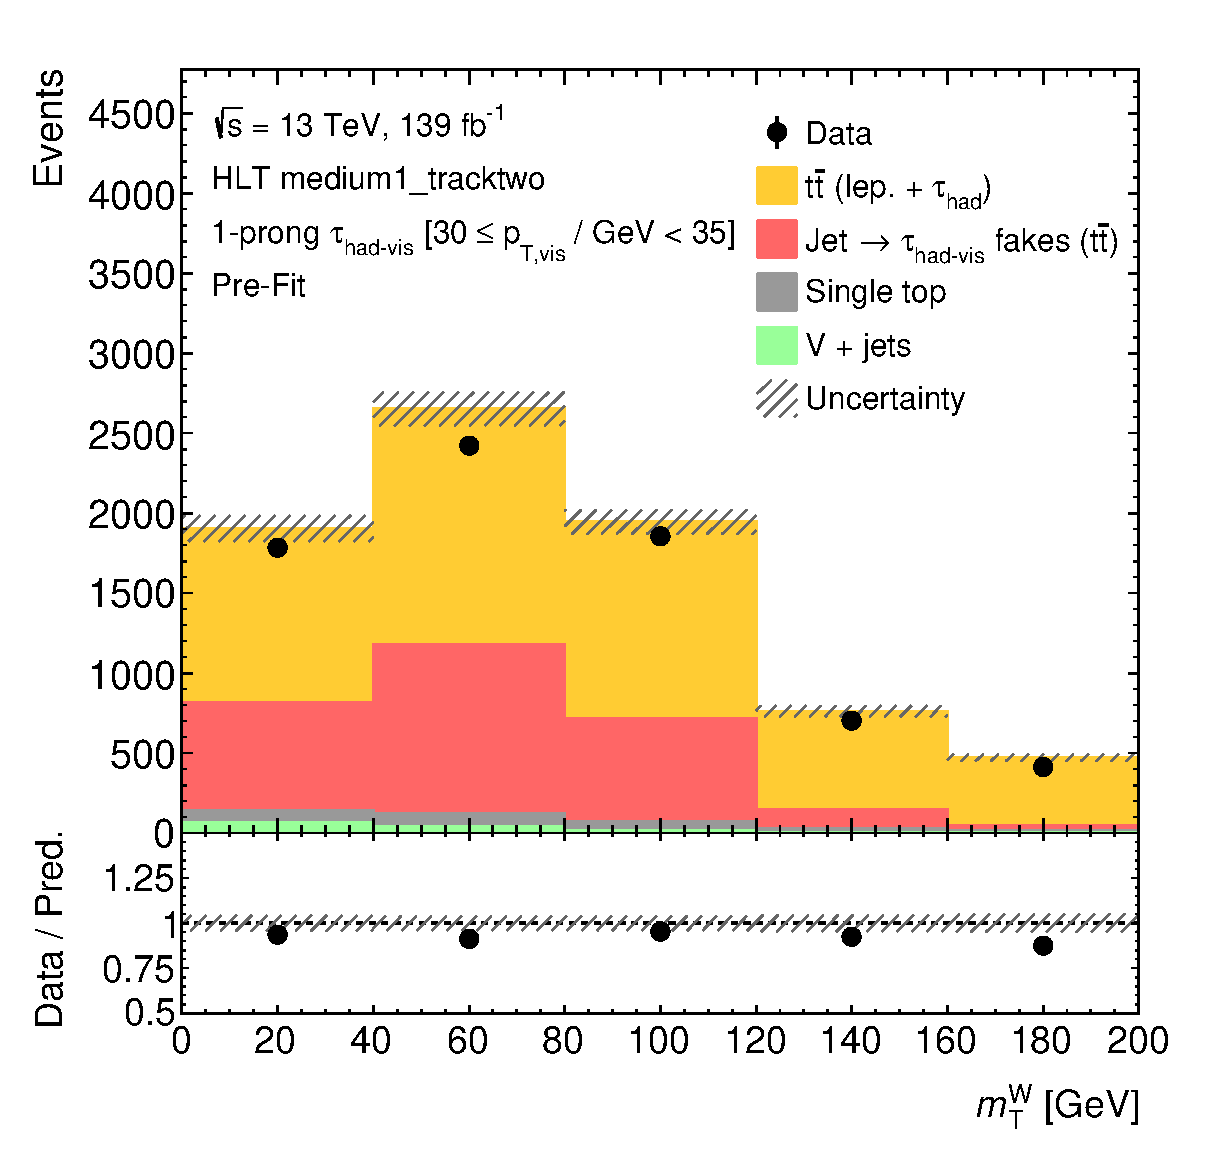
\includegraphics[width=\textwidth]{ttbarSF/tau25/TauPt3035_1P}
    \caption{1-prong \tauhadvis candidates with
      $\SI{30}{\GeV} \leq \pT < \SI{35}{\GeV}$.}
  \end{subfigure}\hfill%
  \begin{subfigure}{.485\textwidth}
    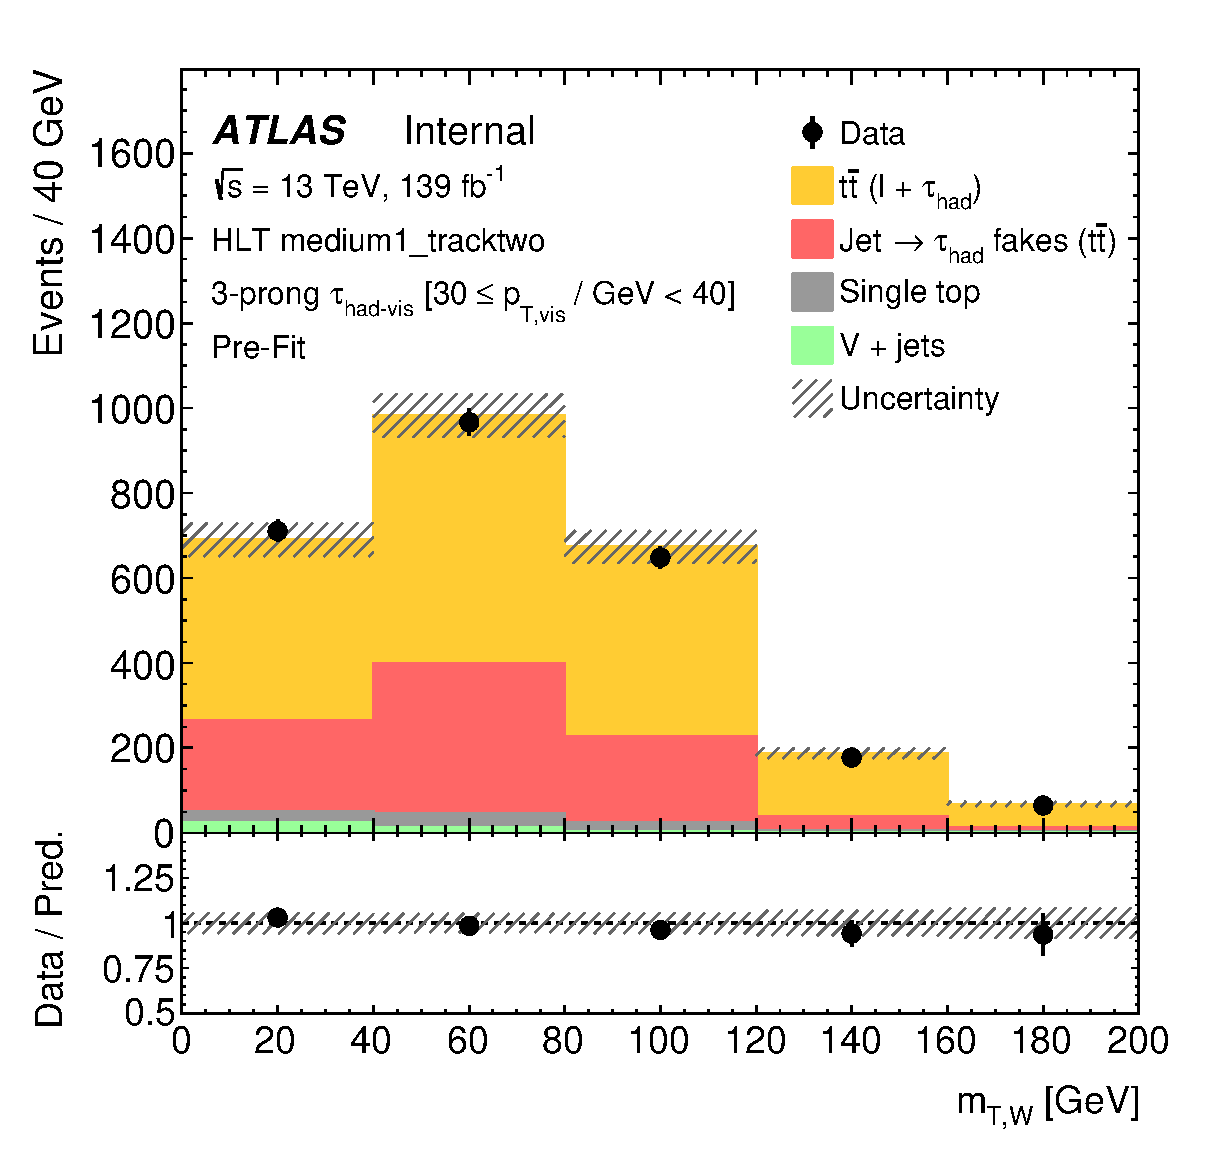
\includegraphics[width=\textwidth]{ttbarSF/tau25/TauPt3040_3P}
    \caption{3-prong \tauhadvis candidates with
      $\SI{30}{\GeV} \leq \pT < \SI{40}{\GeV}$.}
  \end{subfigure}

  \caption{Two exemplary binned \mTW distributions as they enter the
    maximum likelihood estimation procedure to determine the
    \faketauhadvis scale factors. All events are required to pass the
    resurrected trigger decision and trigger-matching of the
    \texttt{HLT\_tau25\_medium1\_tracktwo} chain. Events with
    $\mTW > \SI{200}{\GeV}$ are merged into the last bin of the
    histograms.}%
  \label{fig:ttbarsf_mtw_examples_prefit}
\end{figure}

The normalisation of \ttbar with \faketauhadvis is allowed to vary
freely in every measurement region. The associated normalisation
factors correspond to the \faketauhadvis scale factors of
interest. The \ttbar cross-section is extracted from the fit to data
by allowing the overall normalisation of \ttbar (including \ttbar with
and without \faketauhadvis) to vary freely. The \ttbar normalisation
factor is fully correlated between all subregions entering the
measurement. This approach is taken, as opposed to leaving the \ttbar
normalisation freely floating in every subregion separately, due to
the weak discrimination power of \mTW for small \tauhadvis \pT.


\subsubsection{Uncertainties}

The predicted number of events in bins entering the measurement are
subject to statistical, experimental, and theoretical
uncertainties. These uncertainties can affect the shape and
normalisation of the \mTW distribution in the measurement regions and
the relative acceptance between regions for a given physics
process. Systematic uncertainties affecting the modelling of \ttbar
with true and fake-\tauhadvis in simulation are of primary concern due
to their ability to alter the extracted scale factors. In the
following, a description of the uncertainties is given with a focus of
theoretical modelling uncertainties derived for this
measurement. Detector-related experimental uncertainties are only
briefly summarised, a detailed description following
in~\Cref{sec:uncertainties} when introducing the fit model of the
search for Higgs boson pair production.

Statistical uncertainties arise from the finite size of the simulation
samples used to estimate the physics processes entering this
measurement. These are included in the likelihood function using the
method by Barlow and Beeston~\cite{barlow1993,conway2011} introduced
in \Cref{sec:barlow_beeston}.

Major detector-related experimental uncertainties originate from the
reconstruction and selection of electrons, muons, \tauhadvis and jets.
These uncertainties can affect the reconstructed momenta in scale,
resolution, and direction as well as selection efficiencies of physics
objects for example due to isolation and identification
requirements. When requiring events to pass the resurrected trigger
decision of single-\tauhadvis triggers, calibrations of trigger
selection efficiencies and their associated uncertainties are applied
to \tauhadvis that are matched to a generator-level \tauhad (true
\tauhadvis). Uncertainties on the missing transverse momentum account
for changes in momentum scale and resolution. The uncertainties on
\btag efficiencies and mis-tag rates are obtained from dedicated
calibration measurements performed by the ATLAS collaboration and are
considered in the fit model. Other experimental uncertainties
originating from trigger efficiencies of single lepton triggers,
efficiencies of jet vertex tagging, re-weighting of pile-up conditions
in simulation to match the conditions in Run~2 data, and the
integrated luminosity used to normalise the simulated datasets are
included in the fit.

% https://twiki.cern.ch/twiki/bin/viewauth/AtlasProtected/PmgTopProcesses
Theoretical uncertainties on the acceptance of \ttbar in simulation,
which uses \POWHEGBOX[v2]~\cite{Frixione:2007nw} as a matrix element
(ME) generator interfaced to \PYTHIA[8.230]~\cite{Sjostrand:2014zea}
for the parton shower (PS), need to be estimated. The cross-section of
\ttbar is allowed to vary freely in the fit model, therefore
uncertainties only affecting the normalisation of \ttbar are
omitted. However, uncertainties changing the relative acceptance
between regions (i.e.\ uncertainties depending on \tauhadvis \pT or
decay mode) entering the fit and effects changing the shape of the
\mTW discriminant need to be estimated. The following sources of
uncertainties are considered:
\begin{description}

\item[Hard scatter simulation and NLO+PS matching] The uncertainty on
  the modelling due to the choice of generator describing the hard
  scatter process is estimated by comparing the nominal simulation of
  \ttbar with an alternative setup replacing \POWHEGBOX[v2] with
  \MGNLO as the ME generator. This comparison serves to probe the
  effect of different matching schemes between the NLO matrix element
  and parton shower employed by both
  generators.\footnote{\POWHEGBOX[v2] uses the \POWHEG
    method~\cite{Nason:2004rx,Frixione:2007vw,Alioli:2010xd} and
    \MGNLO the MC@NLO method~\cite{Frixione:2002ik} for NLO+PS
    matching.}

\item[Parton shower and hadronisation model] The uncertainty of the
  modelling of the parton shower and non-perturbative effects is
  estimated by replacing \PYTHIA[8] with \HERWIG[7.0.4] as the PS
  generator.

\item[Missing higher order contributions] The renormalisation
  scale~(\muR) and factorisation scale~(\muF) is doubled (halved) to
  probe the effect of truncating the perturbative expansion in \alphas
  when simulating the hard scatter process. Perturbative QCD
  calculations to sufficiently high order should be approximately
  independent of the choice of scale.

\item[Initial and final state radiation (ISR / FSR)] An uncertainty on
  the emission of ISR is estimated by varying $\alphas^\text{ISR}$ in
  the A14 set of tuned parameters for
  \PYTHIA[8]~\cite{ATL-PHYS-PUB-2014-021}.
  % Tune of the MPI, ISR, FSR parameters in Pythia8
  An estimate of the uncertainty from the modelling of FSR emissions
  is estimated by doubling (halving) the renormalisation scale used
  for FSR branchings in
  \PYTHIA[8]~\cite{Sjostrand:2014zea,Mrenna:2016sih,pythia-variations-online}.
  % https://pythia.org/latest-manual/Variations.html

\item[Damping factor for additional emissions] The damping
  parameter~\hdamp in \POWHEGBOX[v2] is increased to $3 m_\text{top}$
  (from $1.5 m_\text{top}$) and compared with the nominal simulation
  setup. The \hdamp parameter controls the transverse momentum of
  additional radiation when matching \POWHEGBOX[v2] to \PYTHIA[8]
  using the
  \POWHEG-method~\cite{ATL-PHYS-PUB-2016-020,ATL-PHYS-PUB-2020-023}.

\end{description}
% PDF uncertainties were neglected.
The prescriptions to calculate the \ttbar modelling uncertainties are
a revised version of the methodology outlined in
Ref.~\cite{ATL-PHYS-PUB-2020-023} for analyses targeting the
$pp$-collision dataset collected with the ATLAS detector during Run~2
of the LHC.

Variations of the renormalisation and factorisation scales used for
the ME generation are provided by internal re-weighting in
\POWHEGBOX[v2]. Similarly, \PYTHIA[8] provides variations of initial
and final state emissions by varying the renormalisation scales in the
PS by re-weighting~\cite{Mrenna:2016sih,pythia-variations-online}. This
approach allows to estimate uncertainties without changing the
particle-level predictions of the simulation program, thus avoiding
the need to re-run the detector simulation.

Uncertainties derived by performing a two-sample comparison (NLO+PS
matching, PS, \hdamp) are parameterised in \tauhadvis \pT,
reconstructed \tauhadvis decay mode, and \mTW, separately for \ttbar
with true and \faketauhadvis. A smooth functional dependence of these
uncertainties is obtained using least squares fits of polynomials to
the relative change in event yields comparing the alternative with the
nominal sample in bins of \tauhadvis \pT and \mTW. This approach
limits spurious pulls and constraints of the associated nuisance
parameters in the maximum likelihood fit due to statistical
fluctuations of the derived uncertainties. The degree of the fitted
polynomials is determined by leave-one-out cross-validation yielding a
low expected value and variance of the $\chi^2$ statistic.

Dependencies of the uncertainties on \tauhadvis \pT and \mTW are
factorised. First, the effect of the uncertainties on \tauhadvis \pT
is determined by performing the regression on the relative difference
in event yields between both samples binned in \tauhadvis \pT. An
example for the PS variation for true \tauhadvis in 1- and 3-prong
decay modes is shown
in~\Cref{fig:ttbarSF_uncertainty_ps_1p_pt,fig:ttbarSF_uncertainty_ps_3p_pt}. Subsequently,
the nominal event sample is re-weighted using the estimated
\pT-dependency of the uncertainty and the residual non-closure in \mTW
with respect to the variation sample is examined. Generally, the
non-closure is small after taking the \tauhadvis \pT effect of the
variations into account. Minor shape differences are only observed for
the ME and PS generator variations for true \tauhadvis. The
non-closure is parameterised similarly, where non-negligible, and
assigned as an uncertainty fully correlated with the \pT-dependent
effect. Examples of the residual non-closure in \mTW after
\pT-re-weighting is shown
in~\Cref{fig:ttbarSF_uncertainty_ps_1p_mtw,fig:ttbarSF_uncertainty_ps_3p_mtw}. Variations
of the damping parameter, $\hdamp$, show no significant effect on the
shape of the \tauhadvis \pT or \mTW distributions, thus uncertainties
are only assigned on the relative normalisation between categories
defined by \tauhadvis decay mode and truth-matching to generator-level
\tauhad.

% Subsequently, the nominal sample is reweighted using the estimated
% \pT-dependency and the residual non-closure in \mTW is examined. The
% non-closure in \mTW is small after taking the \tauhadvis \pT effect of
% the variation into account. Minor shape differences are only observed
% for the ME and PS generation variations for true \tauhadvis. An
% example is shown
% in~\Cref{fig:ttbarSF_uncertainty_ps_1p_mtw,fig:ttbarSF_uncertainty_ps_3p_mtw}
% for the PS variation. The non-closure is assigned as an uncertainty
% fully correlated with the \pT effect. The variations of the damping
% parameter related to the NLO+PS matching in \POWHEG show no
% statistically significant effect depending on \tauhadvis \pT or
% \mTW. Thus only an uncertainty on the relative normalisation between
% categories is assigned.

\begin{figure}[htbp]
  \centering

  \begin{subfigure}[t]{.48\textwidth}
    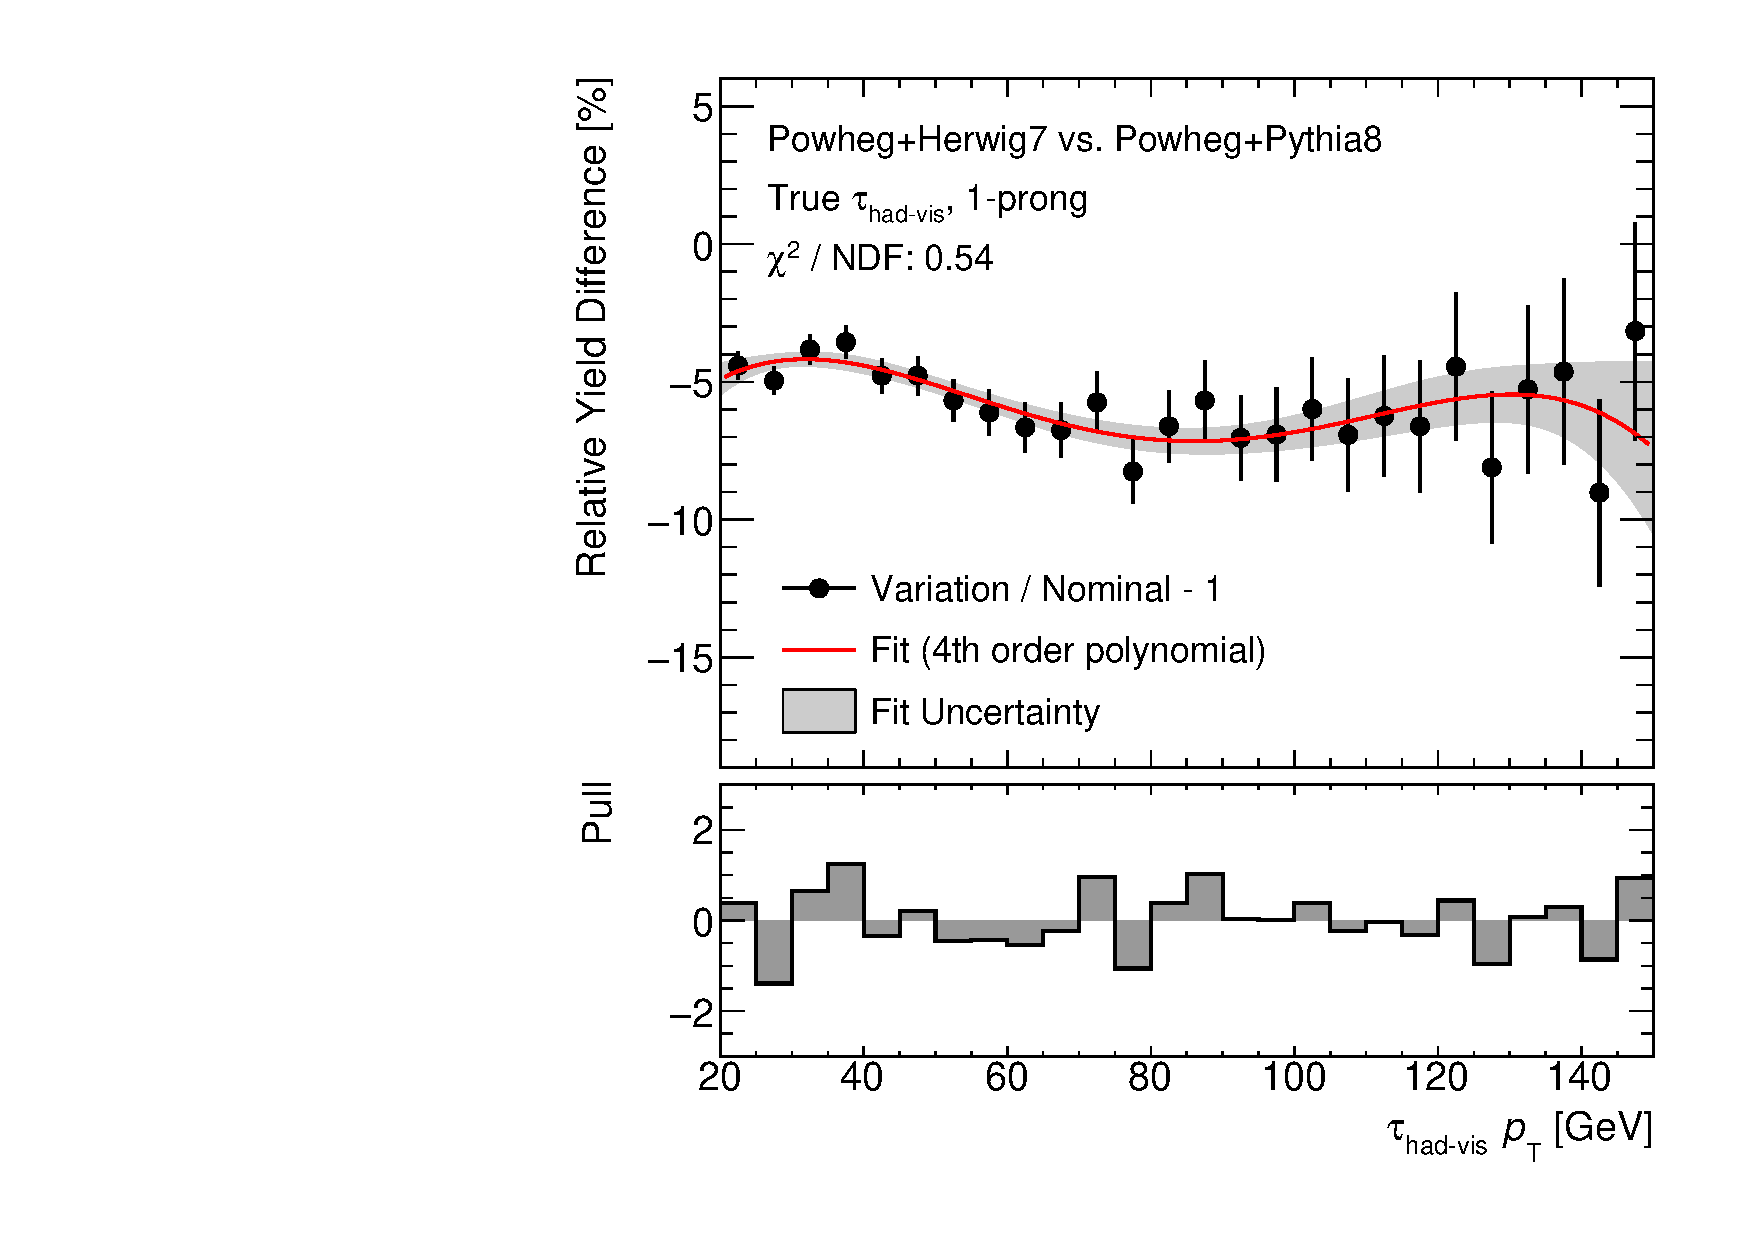
\includegraphics[width=\textwidth]{ttbarSF/uncertainties/ps_true_1p_pt}
    \caption{Impact of the PS variation on \tauhadvis \pT for 1-prong
      \tauhadvis.}
    \label{fig:ttbarSF_uncertainty_ps_1p_pt}
  \end{subfigure}\hfill%
  \begin{subfigure}[t]{.48\textwidth}
    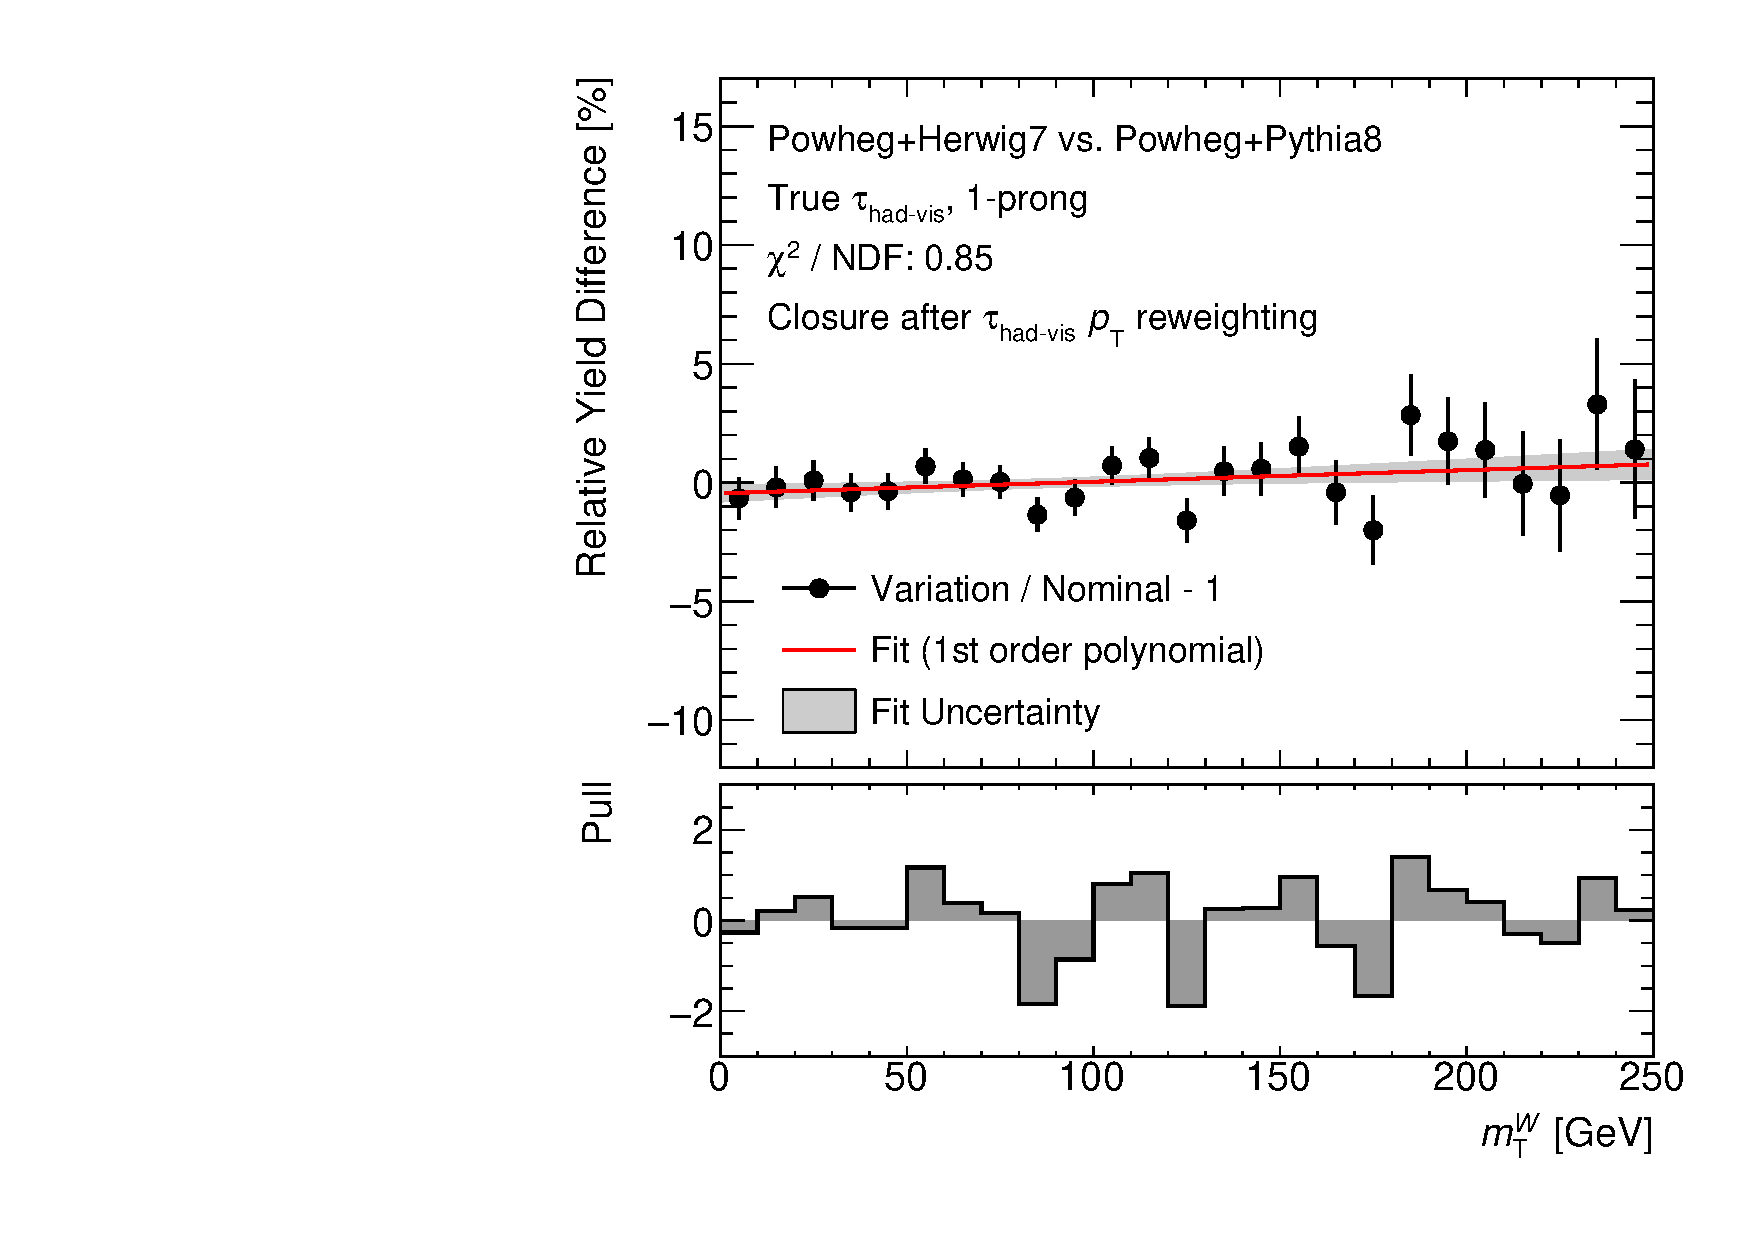
\includegraphics[width=\textwidth]{ttbarSF/uncertainties/ps_true_1p_mtw}
    \caption{Non-closure in \mTW of the PS variation for 1-prong
      \tauhadvis after re-weighting the nominal simulation sample.}
    \label{fig:ttbarSF_uncertainty_ps_1p_mtw}
  \end{subfigure}

  \vspace{0.5em}

  \begin{subfigure}[t]{.48\textwidth}
    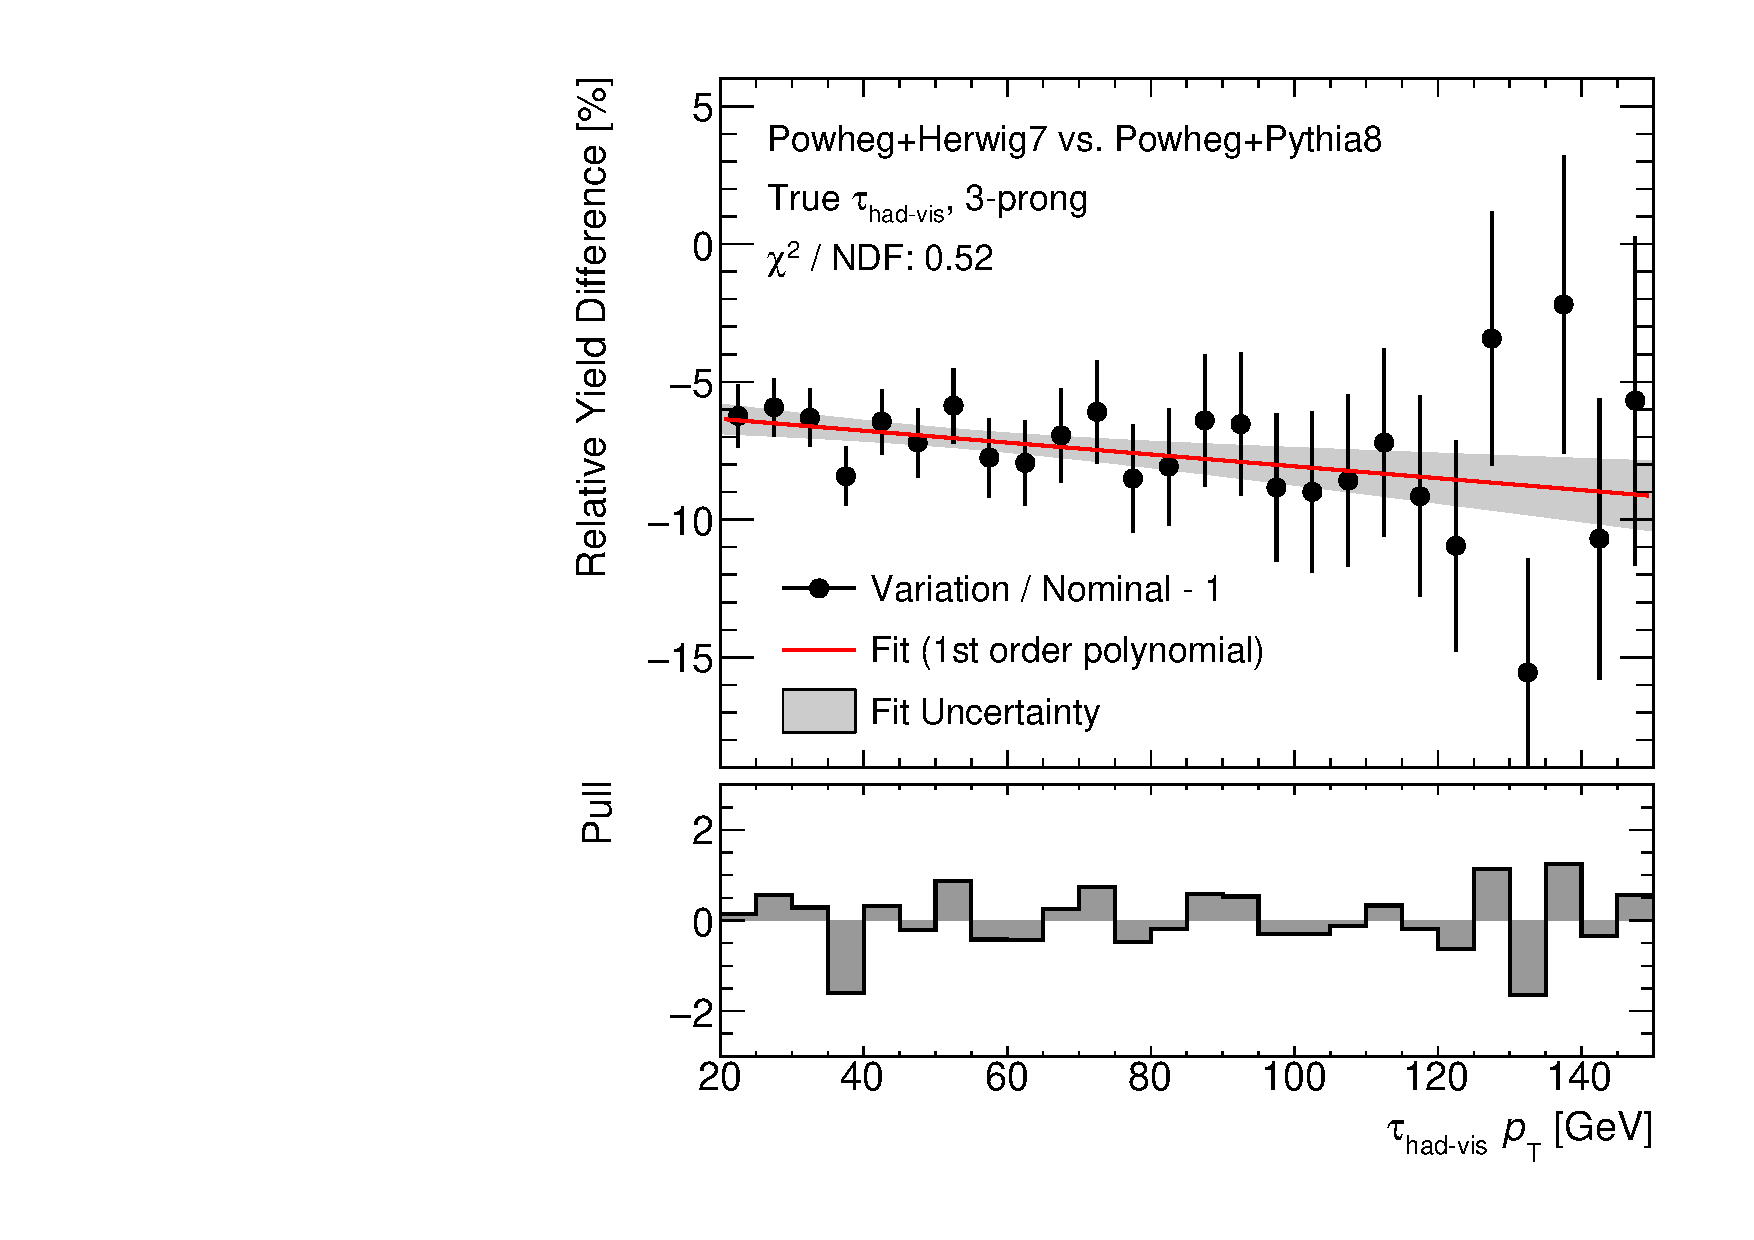
\includegraphics[width=\textwidth]{ttbarSF/uncertainties/ps_true_3p_pt}
    \caption{Impact of the PS variation on \tauhadvis \pT for 3-prong
      \tauhadvis.}
    \label{fig:ttbarSF_uncertainty_ps_3p_pt}
  \end{subfigure}\hfill%
  \begin{subfigure}[t]{.48\textwidth}
    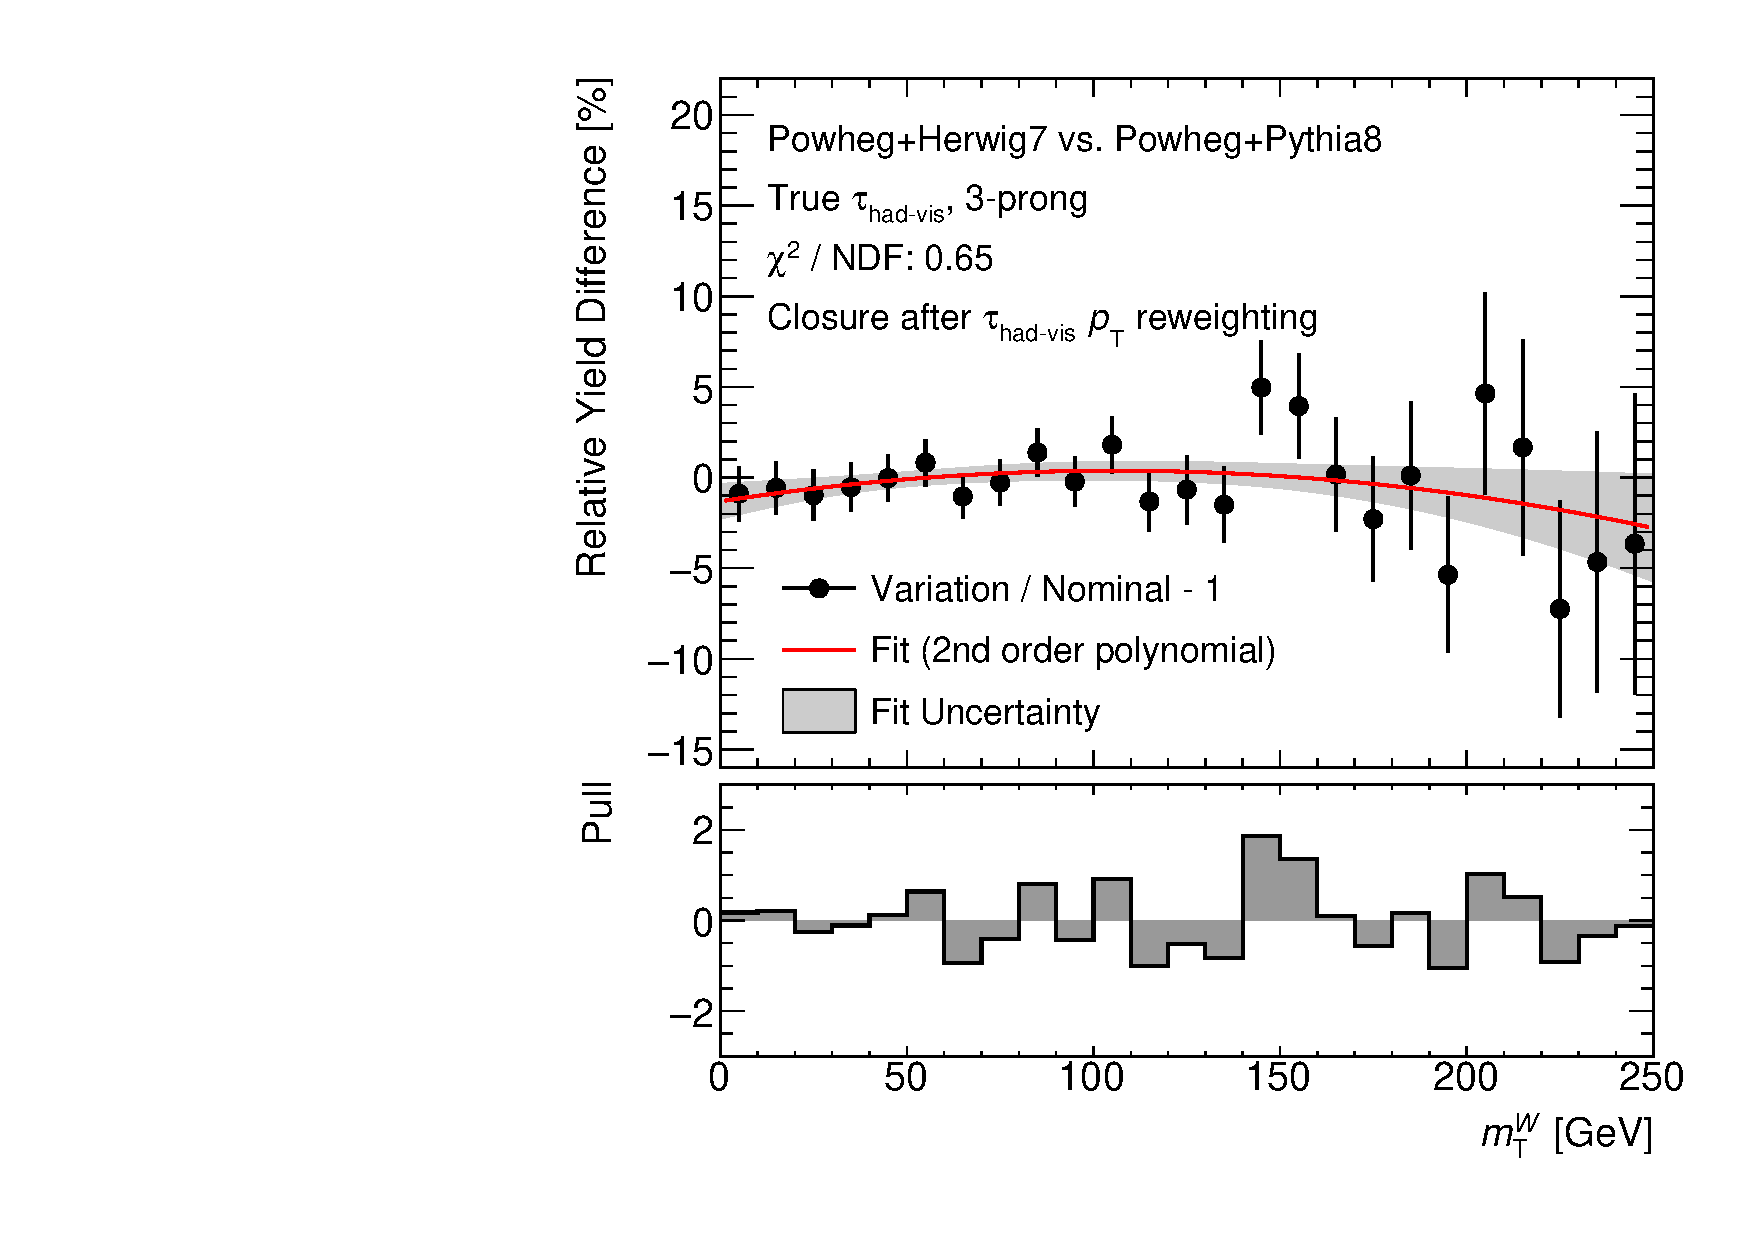
\includegraphics[width=\textwidth]{ttbarSF/uncertainties/ps_true_3p_mtw}
    \caption{Non-closure in \mTW of the PS variation for 3-prong
      \tauhadvis after re-weighting the nominal simulation sample.}
    \label{fig:ttbarSF_uncertainty_ps_3p_mtw}
  \end{subfigure}

  \caption{The effect of the parton shower and hadronisation model
    uncertainty on the relative difference in event yield, defined as
    $N_{\text{syst.}} / N_{\text{nom.}} - 1$ with $N_{\text{syst.}}$
    and $N_{\text{nom.}}$ being the event yield in a given bin for the
    systematic variation and nominal event sample, derived from a
    two-sample comparison of \POWHEGBOX[v2]+~\PYTHIA[8] (nominal) and
    \POWHEGBOX[v2]+~\HERWIG[7] (variation). Shown are the uncertainty
    for 1-prong (a,b) and 3-prong (c,d) \tauhadvis matched to \tauhad
    at generator-level (true \tauhadvis). The lower threshold on
    \tauhadvis \pT was relaxed to \SI{20}{\GeV} (from \SI{25}{\GeV})
    compared to the top control region.}%
  \label{fig:ttbarSF_uncertainty_ps}
\end{figure}

% The alternative parton shower has the largest effect on the
% modelling of \faketauhadvis.

Acceptance uncertainties on \ttbar with \faketauhadvis are assigned as
shape-only uncertainties in all measurement regions since the
normalisation of this component is extracted in the likelihood fit.
In contrast, the normalisation of \ttbar with true \tauhadvis is not
extracted in each measurement region separately. Therefore, both the
normalisation and the shape effect of the acceptance uncertainties are
propagated to the fit for \ttbar with true \tauhadvis.

A reduced set of theory uncertainties for minor backgrounds is
considered. For the production of single top-quarks, the uncertainties
on the cross-section are included in the fit model. Due to the known
normalisation discrepancy in \Vjets in the presence of jets
originating from heavy flavour, an uncertainty of \SI{30}{\percent} is
applied to the overall normalisation of the process.

The effect of uncertainties on the predicted rates are parameterised by
nuisance parameters that enter the maximum likelihood fit with
Gaussian constraint terms. Uncertainties arising from the same source
are assumed to be fully correlated across all regions and
bins. Uncertainties derived from two-sample comparisons are
symmetrised.


\subsubsection{Measurement Results}

The measured scale factors for \faketauhadvis in \ttbar simulation are
shown in \Cref{fig:ttbarSF_postfit_SF}. The measurement shows varying
agreement between the nominal prediction from simulation and the
data-driven method that depends on the \tauhadvis transverse momentum
and the applied \tauid criteria. The size of the extracted correction
can reach up to \SI{50}{\percent} at high \tauhadvis \pT where
simulation overestimates the contribution of \faketauhadvis in \ttbar.

\begin{figure}[htbp]
  \centering

  \begin{subfigure}[t]{.495\textwidth}
    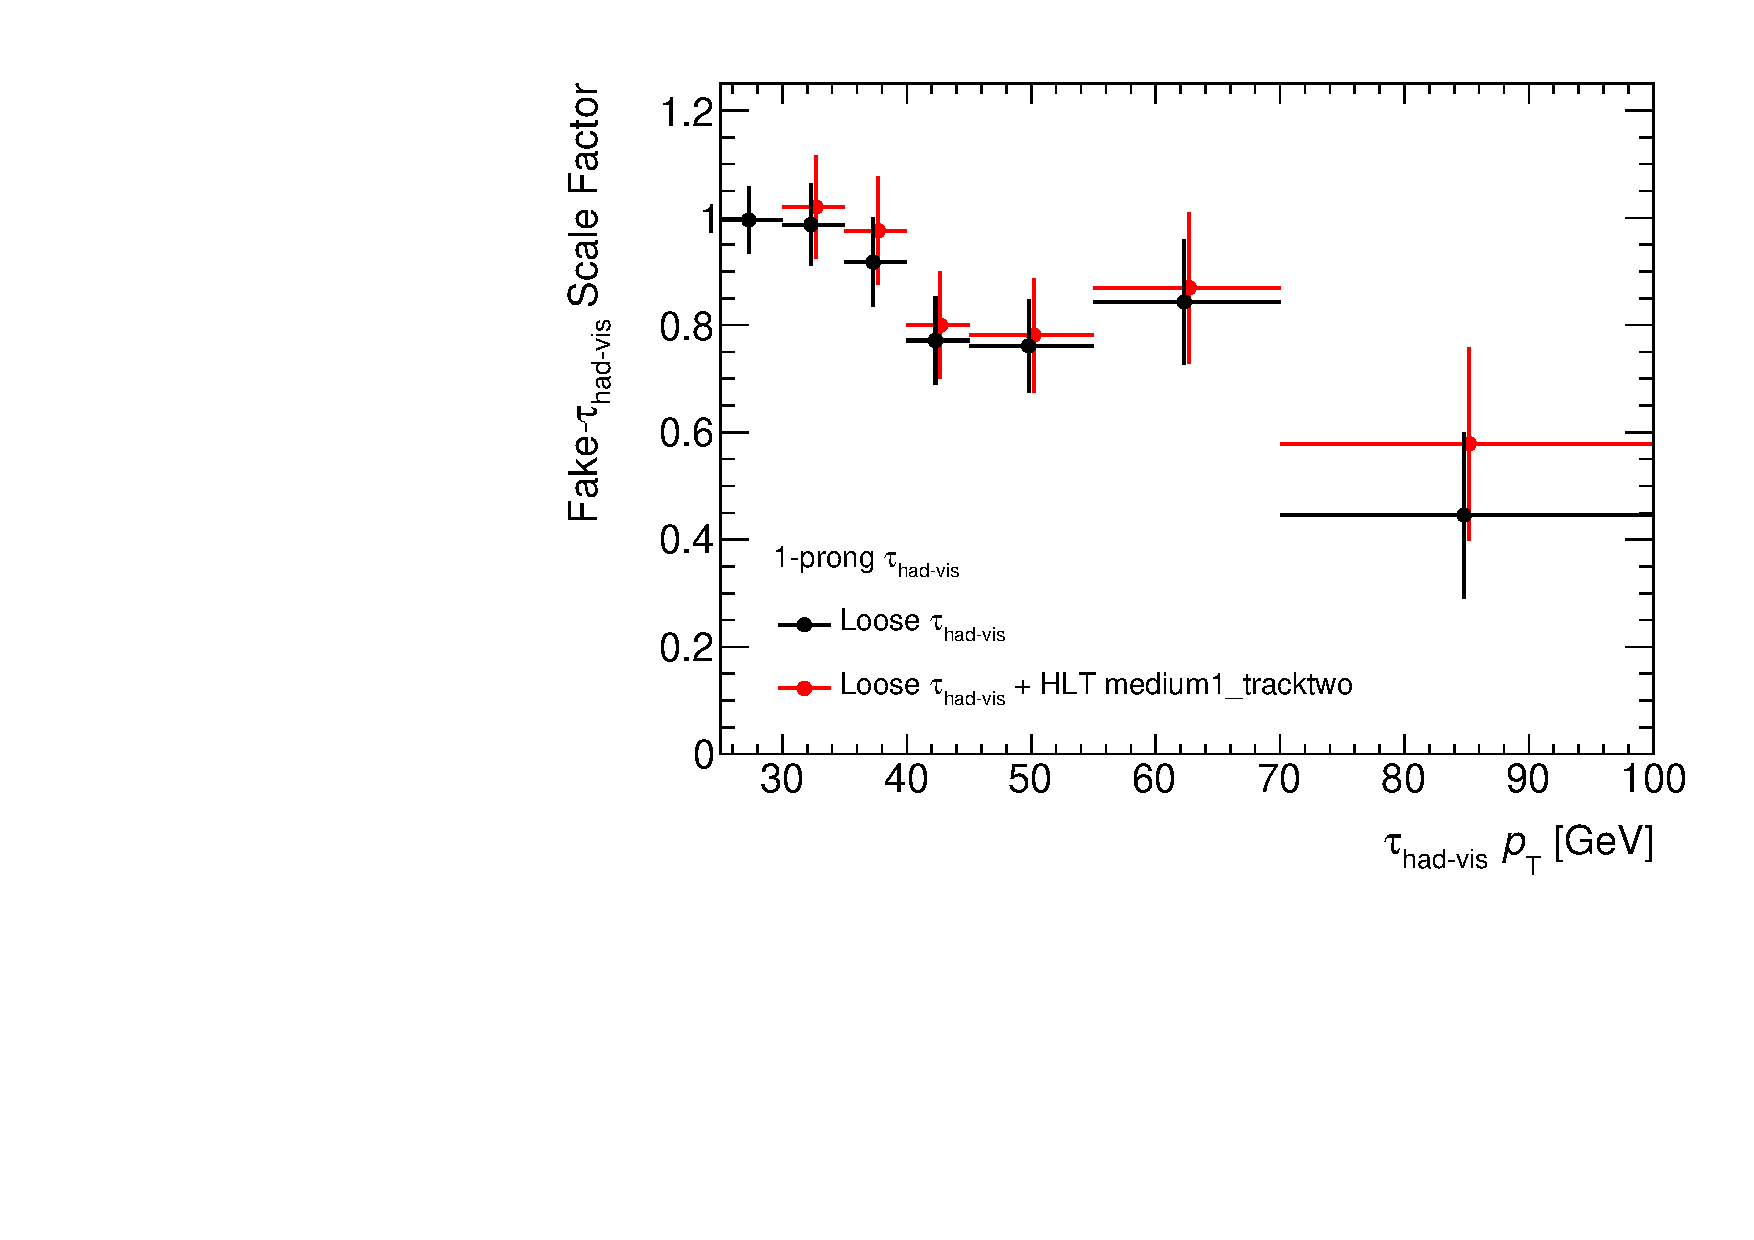
\includegraphics[width=\textwidth]{ttbarSF/ttbarSF_offl_tau25_1p}
    \caption{}
    \label{fig:ttbarSF_postfit_SF_a}
  \end{subfigure}\hfill%
  \begin{subfigure}[t]{.495\textwidth}
    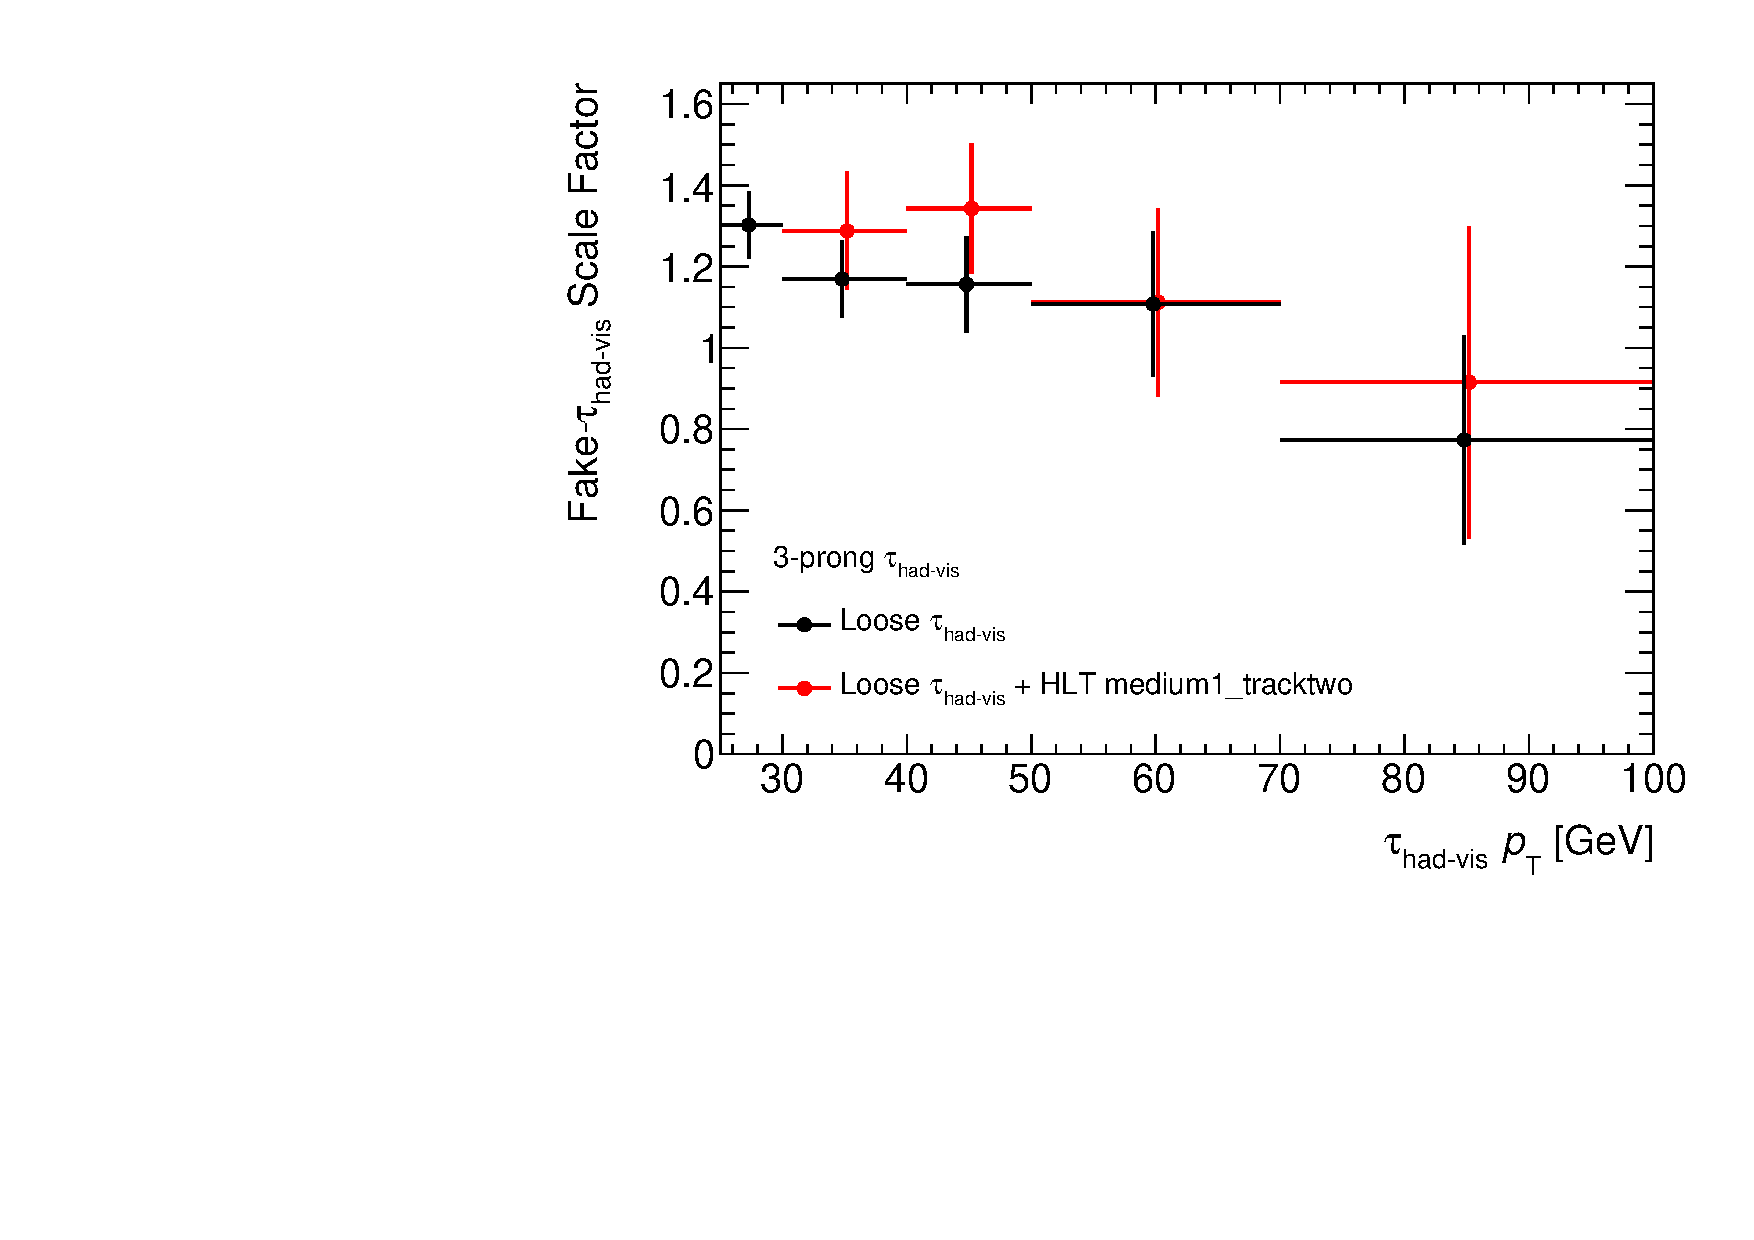
\includegraphics[width=\textwidth]{ttbarSF/ttbarSF_offl_tau25_3p}
    \caption{}
    \label{fig:ttbarSF_postfit_SF_b}
  \end{subfigure}

  \begin{subfigure}[t]{.495\textwidth}
    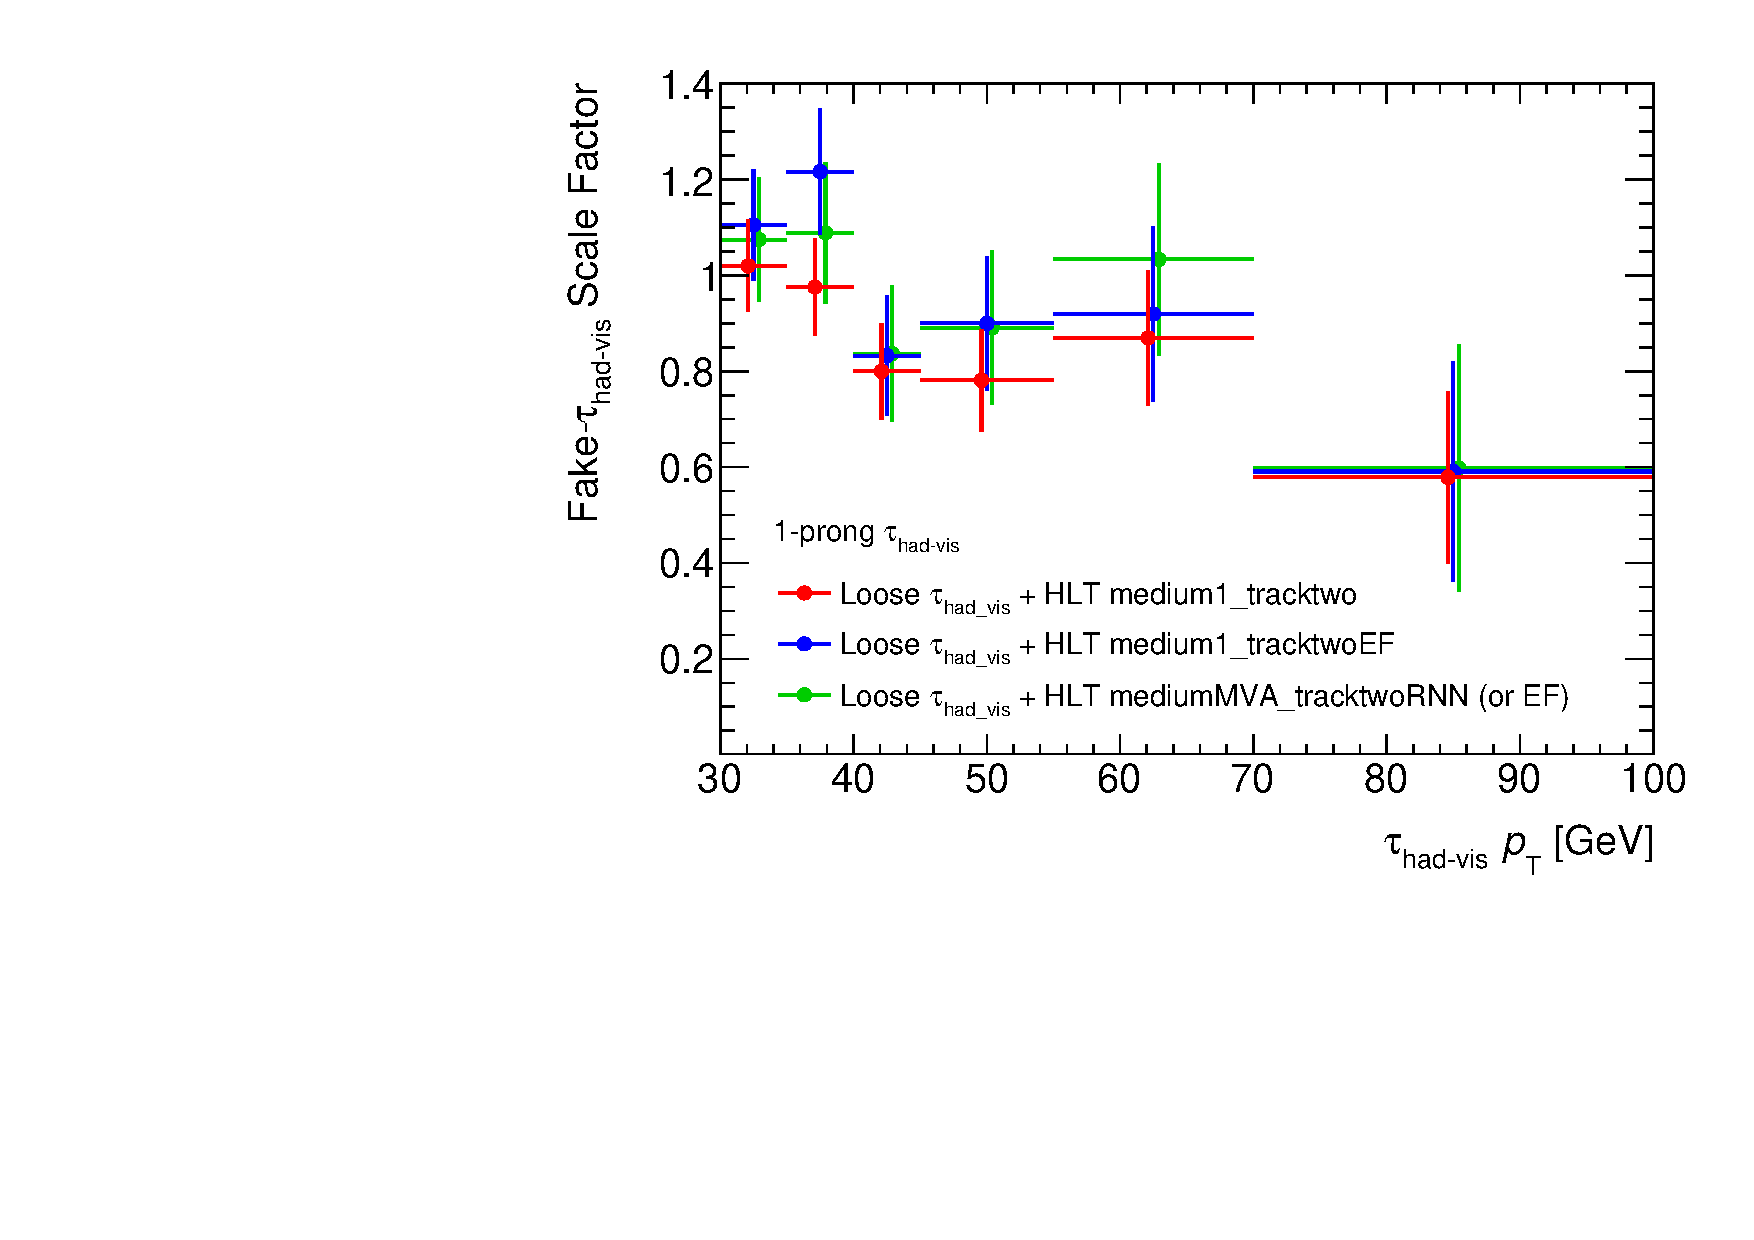
\includegraphics[width=\textwidth]{ttbarSF/ttbarSF_tau25_1p}
    \caption{}
    \label{fig:ttbarSF_postfit_SF_c}
  \end{subfigure}\hfill%
  \begin{subfigure}[t]{.495\textwidth}
    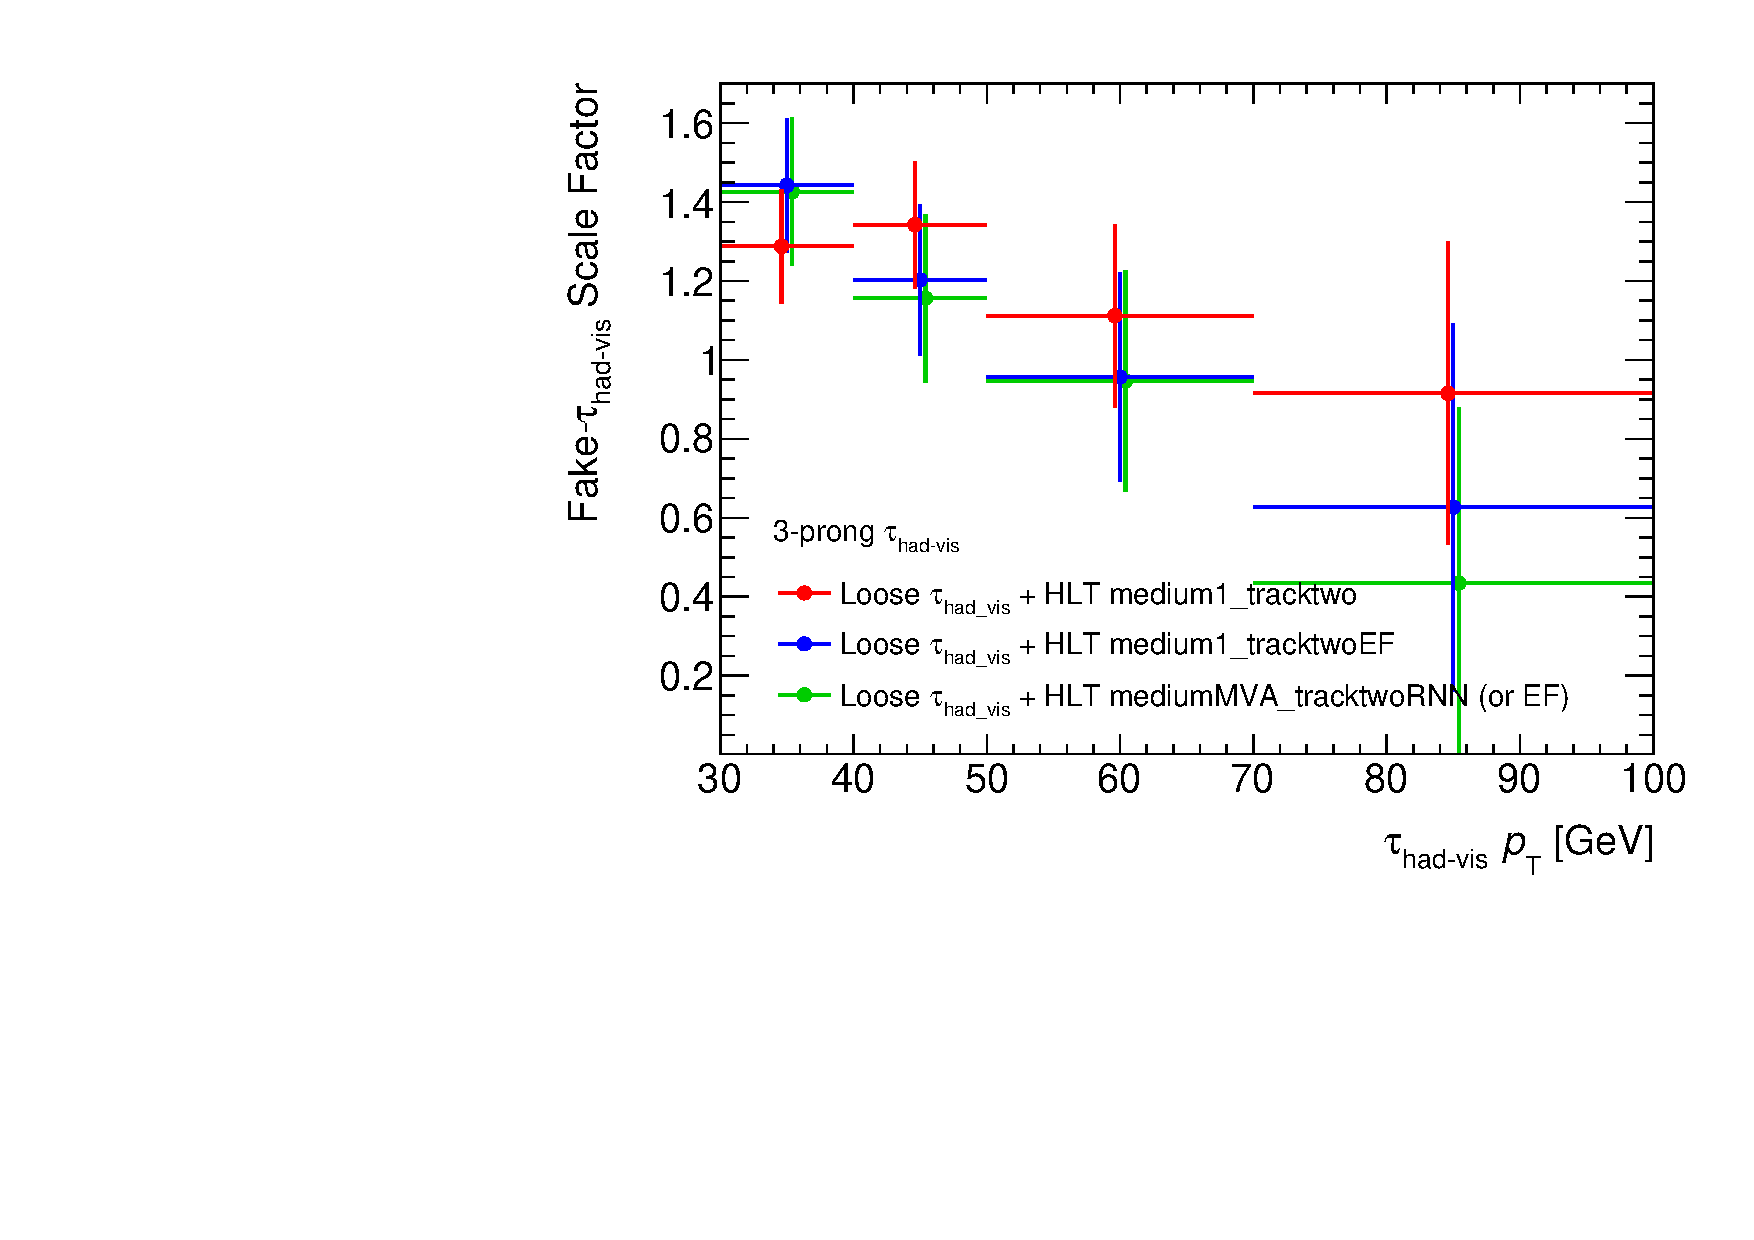
\includegraphics[width=\textwidth]{ttbarSF/ttbarSF_tau25_3p}
    \caption{}
    \label{fig:ttbarSF_postfit_SF_d}
  \end{subfigure}

  \caption{Measured \faketauhadvis scale factors for simulated \ttbar
    (\POWHEGBOX[v2] + \PYTHIA[8]) separated by \tauhadvis
    identification criteria applied in this analysis. A comparison of
    \faketauhadvis scale factors measured with loose offline \tauid
    only and with both loose offline and HLT \tauid is shown in (a)
    and (b) for 1- and 3-prong \tauhadvis candidates, respectively.
    Figures (c) and (d) compare the effect of different HLT
    identification algorithms on the extracted scale factors. In all
    cases, the last bin summarises the scale factors for \tauhadvis
    with $\pT \geq \SI{70}{\GeV}$.  The markers are shifted from the
    geometrical bin centre for illustration purposes only.}%
  \label{fig:ttbarSF_postfit_SF}
\end{figure}

For \faketauhadvis reconstructed as 1-prong \tauhadvis candidates,
depicted in~\Cref{fig:ttbarSF_postfit_SF_a,fig:ttbarSF_postfit_SF_c},
the scale factor corrections are of the order of \SI{20}{\percent} in
the low and intermediate transverse momentum regime
($\pT < \SI{70}{\GeV}$). The extracted scale factors show no strong
dependence on whether candidates pass the selections applied by
\tauhadvis triggers or the particular trigger chain used.

In~\Cref{fig:ttbarSF_postfit_SF_b,fig:ttbarSF_postfit_SF_d} the
measured scale factors for \faketauhadvis reconstructed as 3-prong
candidates are shown. In this case, the contribution of \faketauhadvis
in the low and intermediate \tauhadvis~\pT region is underestimated by
simulation, requiring corrections of about
\SIrange{20}{40}{\percent}. At high transverse momenta simulation
tends to overestimate the \faketauhadvis contribution, although with
large uncertainties from the scale factor measurement. The
uncertainties are magnified for the \texttt{medium1\_tracktwoEF} and
\texttt{mediumMVA\_tracktwoRNN} chains since only partial datasets
containing the resurrected trigger decision are available.

Pulls and constraints of nuisance parameters are examined for all
scale factor measurements\todo{Appendix?}. The nuisance parameter
estimates agree within uncertainties with the central values of their
auxiliary measurements. Few instances are observed where the scale
factor measurement puts more stringent constraints on nuisance
parameters than expected from the prior estimation of the associated
uncertainty. All constrained parameters have post-fit uncertainties
larger than \SI{70}{\percent} with respect to the uncertainty prior to
the fit, indicating only mild constraints.

The largest nuisance parameter constraints, in the following given as
the ratio of post- to pre-fit uncertainty, are observed for the
\pTmissAbs scale uncertainty~(\SI{70}{\percent}), the ME / PS
modelling uncertainties on \ttbar~(\SI{75}{\percent}), and \tauhadvis
energy scale uncertainty~(\SI{80}{\percent}). The \mTW discriminant is
sensitive to the modelling of \pTmissAbs, thus some power to constrain
nuisance parameters related to the modelling of \pTmissAbs in
simulation is expected. Similarly, the SF-CR selects a large number of
\ttbar events with high purity, consequently allowing to constrain the
modelling uncertainties that are derived from two-sample
comparisons. Finally, the measurements providing uncertainties on the
\tauhadvis energy scale are performed in $Z \ra \tau_{\mu} \tauhad$
tag-and-probe~\cite{ATLAS-CONF-2017-029} which provides probe
\tauhadvis with a softer transverse momentum spectrum compared to
\tauhadvis produced in \ttbar events. With the binning of the
measurement in \tauhadvis \pT, it is expected that the uncertainties
on the \tauhadvis energy scale, particularly at high \tauhadvis~\pT,
can be constrained by this measurement. % It cannot be fully excluded,
% however, that these constraints arise from a lack of flexibility of
% the fit model.

The \tauhadvis \pT and \mTW distributions are shown in
\Cref{fig:ttbarSF_postfit_ptmtw} after the fit in the SF-CR with the
additional trigger-matching requirement to the
\texttt{HLT\_tau25\_medium1\_tracktwo} single-\tauhadvis
trigger. Decent agreement is observed between the background
prediction and the observed data.

% \todo[inline]{This measurement can provide a correction as well as a
%   measurement-driven estimate of the uncertainties of
%   \faketauhadvis. Although the uncertainties seem large at high
%   momenta, the abundance of events where this is relevant is small.}

\begin{figure}[htbp]
  \centering

  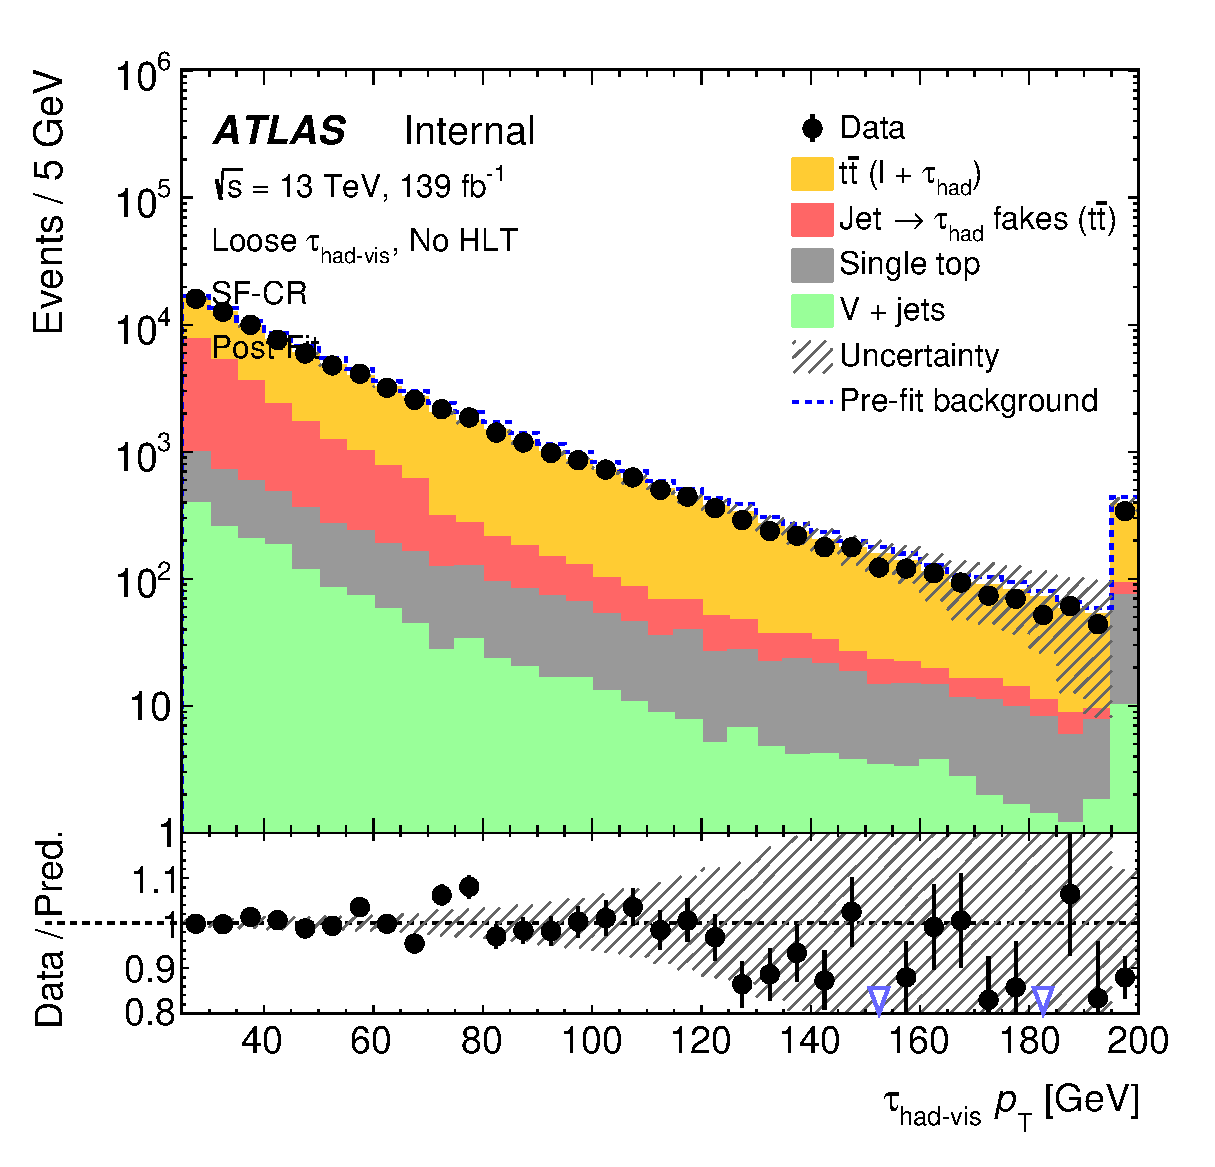
\includegraphics[width=0.49\textwidth]{ttbarSF/postfit_sfcr/PTVR_postFit}
  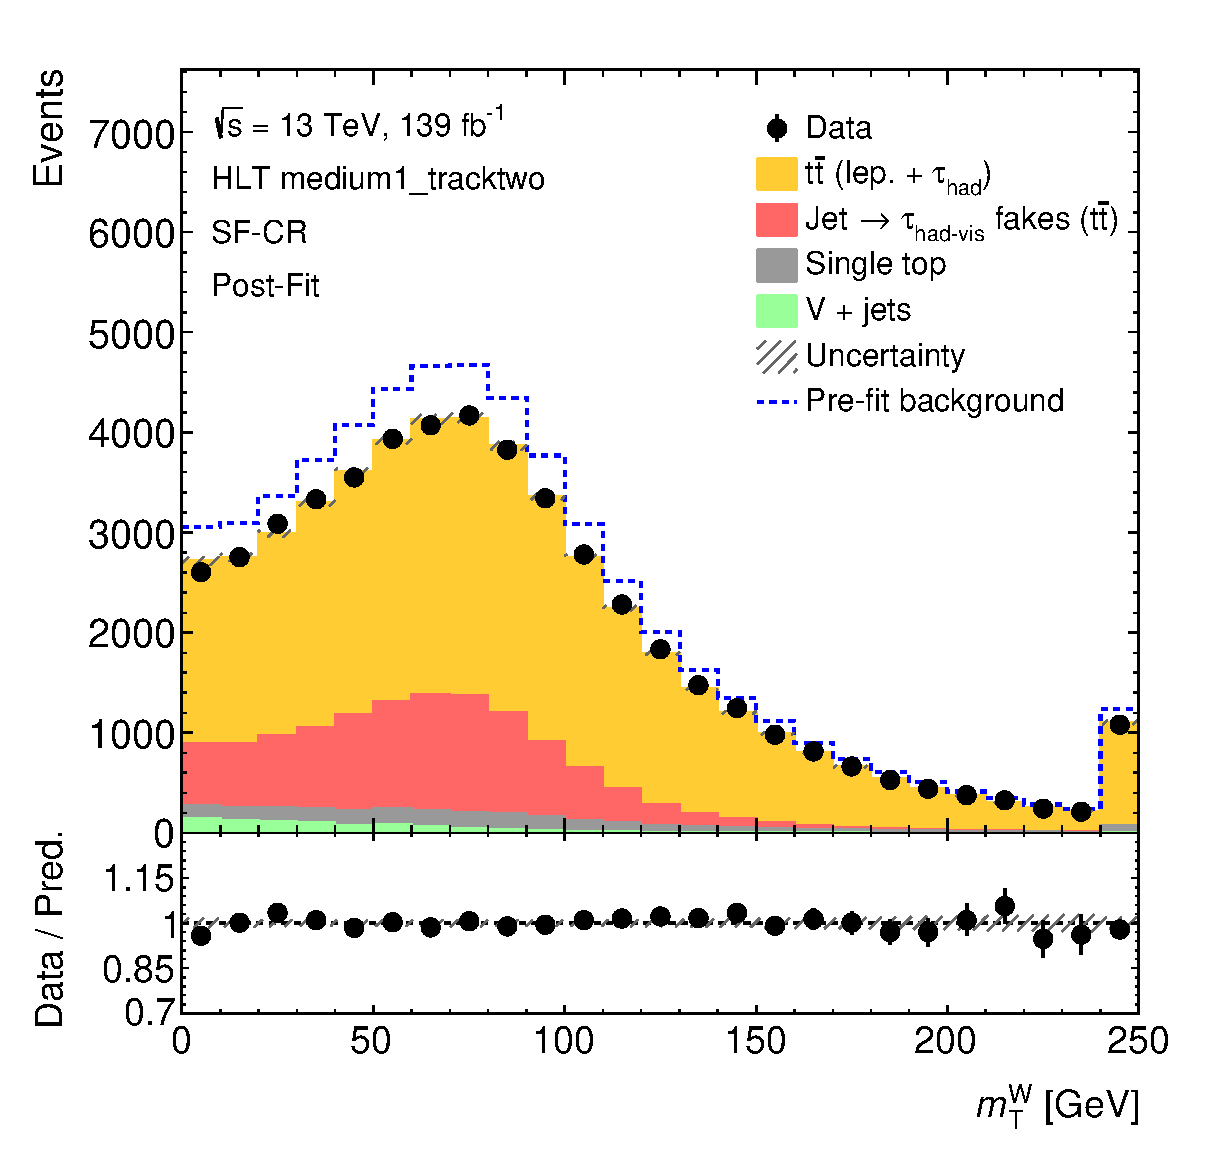
\includegraphics[width=0.49\textwidth]{ttbarSF/postfit_sfcr/MTWVR_postFit}

  \caption{Post-fit distribution of \tauhadvis \pT and \mTW in the
    scale factor control region after requiring the \tauhadvis to be
    matched to the \texttt{HLT\_tau25\_medium1\_tracktwo}
    trigger. Events with \tauhadvis \pT (\mTW) larger than
    \SI{200}{\GeV} (\SI{250}{\GeV}) are merged into the last bin. The
    uncertainty band contains all statistical and systematic
    uncertainties, including post-fit uncertainties on \faketauhadvis
    scale factors and the \ttbar normalisation factor.}
  \label{fig:ttbarSF_postfit_ptmtw}
\end{figure}

The fit model introduces large anti-correlations between the overall
\ttbar normalisation and the extracted scale factors for \ttbar with
\faketauhadvis. An exemplary correlation matrix for one measurement is
shown in~\Cref{fig:ttbarSF_corr_matrix} showing the most relevant
correlations between parameters of interest and nuisance parameters.
The anti-correlations are a result of the limited discrimination power
of \mTW in distinguishing between \ttbar with true- and
\faketauhadvis, which is especially poor for low \tauhadvis transverse
momenta. Thus a change in the overall \ttbar normalisation, affecting
both \ttbar with true and \faketauhadvis, can be partially compensated
by an increase in the \faketauhadvis scale factors. This coupling
between \faketauhadvis scale factors and \ttbar normalisation
introduces large positive correlations also between the scale factors
themselves.

\begin{figure}[htbp]
  \centering

  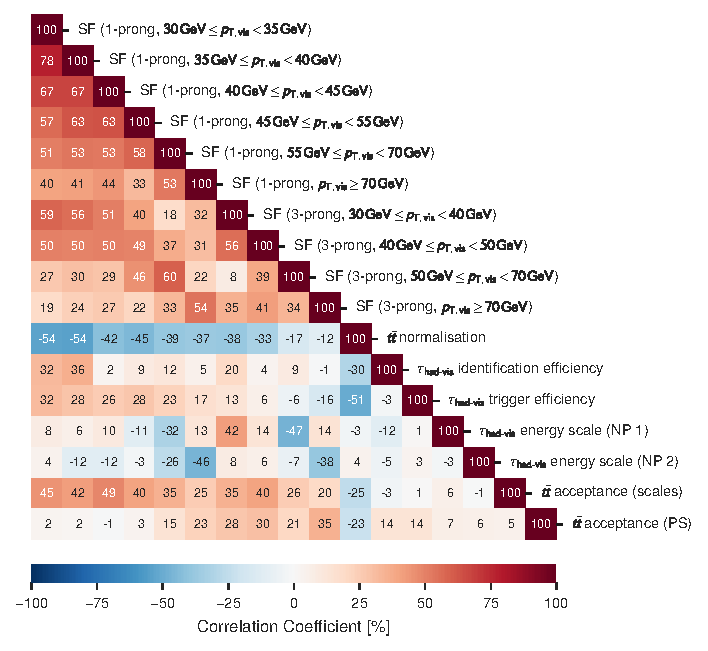
\includegraphics[scale=0.88]{ttbarSF/correlation_matrix}

  \caption{Post-fit correlation matrix between selected parameters of
    the fit model for the \faketauhadvis scale factor measurement
    after matching \tauhadvis to the
    \texttt{HLT\_tau25\_medium1\_tracktwo} trigger. A reduced number
    of nuisance parameters is shown for illustration
    purposes. Nuisance parameters are included if the absolute value
    of its correlation coefficient exceeds \SI{30}{\percent} with at
    least one parameter of interest.}%
  \label{fig:ttbarSF_corr_matrix}
\end{figure}

Correlations between the extracted scale factors need to be taken into
account when propagating the measurement uncertainties to the estimate
of \ttbar with \faketauhadvis in the \hadhad signal region. A way to
achieve this is by providing decorrelated variations of the
measurement that jointly explain the total uncertainty of all scale
factors. These sets of scale factor variations can be used to
propagate the uncertainties without having to account for
correlations.

A decorrelated set of variations can be obtained by a linear
transformation procedure of the $N$ measured scale factors. The
transformation is obtained by diagonalising the post-fit scale factor
covariance matrix, resulting in a set of eigenvectors and
eigenvalues. The eigenvectors provide an alternative basis in which
the measurement is described by $N$~linear combinations of scale
factors with diagonal covariance matrix. The eigenvalues correspond to
the variance explained by certain linear combinations of scale
factors. %
% The covariance between two different linear combinations is
% zero by construction and the eigenvalues describe the variance of
% individual linear combinations.
In the frame with diagonal covariance matrix, the scale factor
measurement is varied by performing $\pm 1 \sigma$ variations, then
transforming the resulting variations back to the original, physically
interpretable frame. This procedure yields $N$ systematic variations
of the scale factor measurement each with an up- and
down-variation.\footnote{In this context, calling a variation ``up''
  or ``down'' has no concrete physical meaning.} The variations are
ordered by descending variance in the diagonal frame, yielding
variations that are roughly decreasing in their impact on the total
\ttbarFakes background estimate. An example of this decorrelation
approach is shown in~\Cref{fig:ttbarSF_eigenvariations}. The effect of
large correlations between scale factors can be seen in the leading
variation (\texttt{EIGEN0}) as a systematic shift of the variation in
all bins with respect to the nominal result. In contrast, the
variation explaining the least variance (\texttt{EIGEN9}) only alters
the scale factors for 1-prong \faketauhadvis with low transverse
momenta.

\begin{figure}[htbp]
  \centering

  \begin{subfigure}[t]{.495\textwidth}
    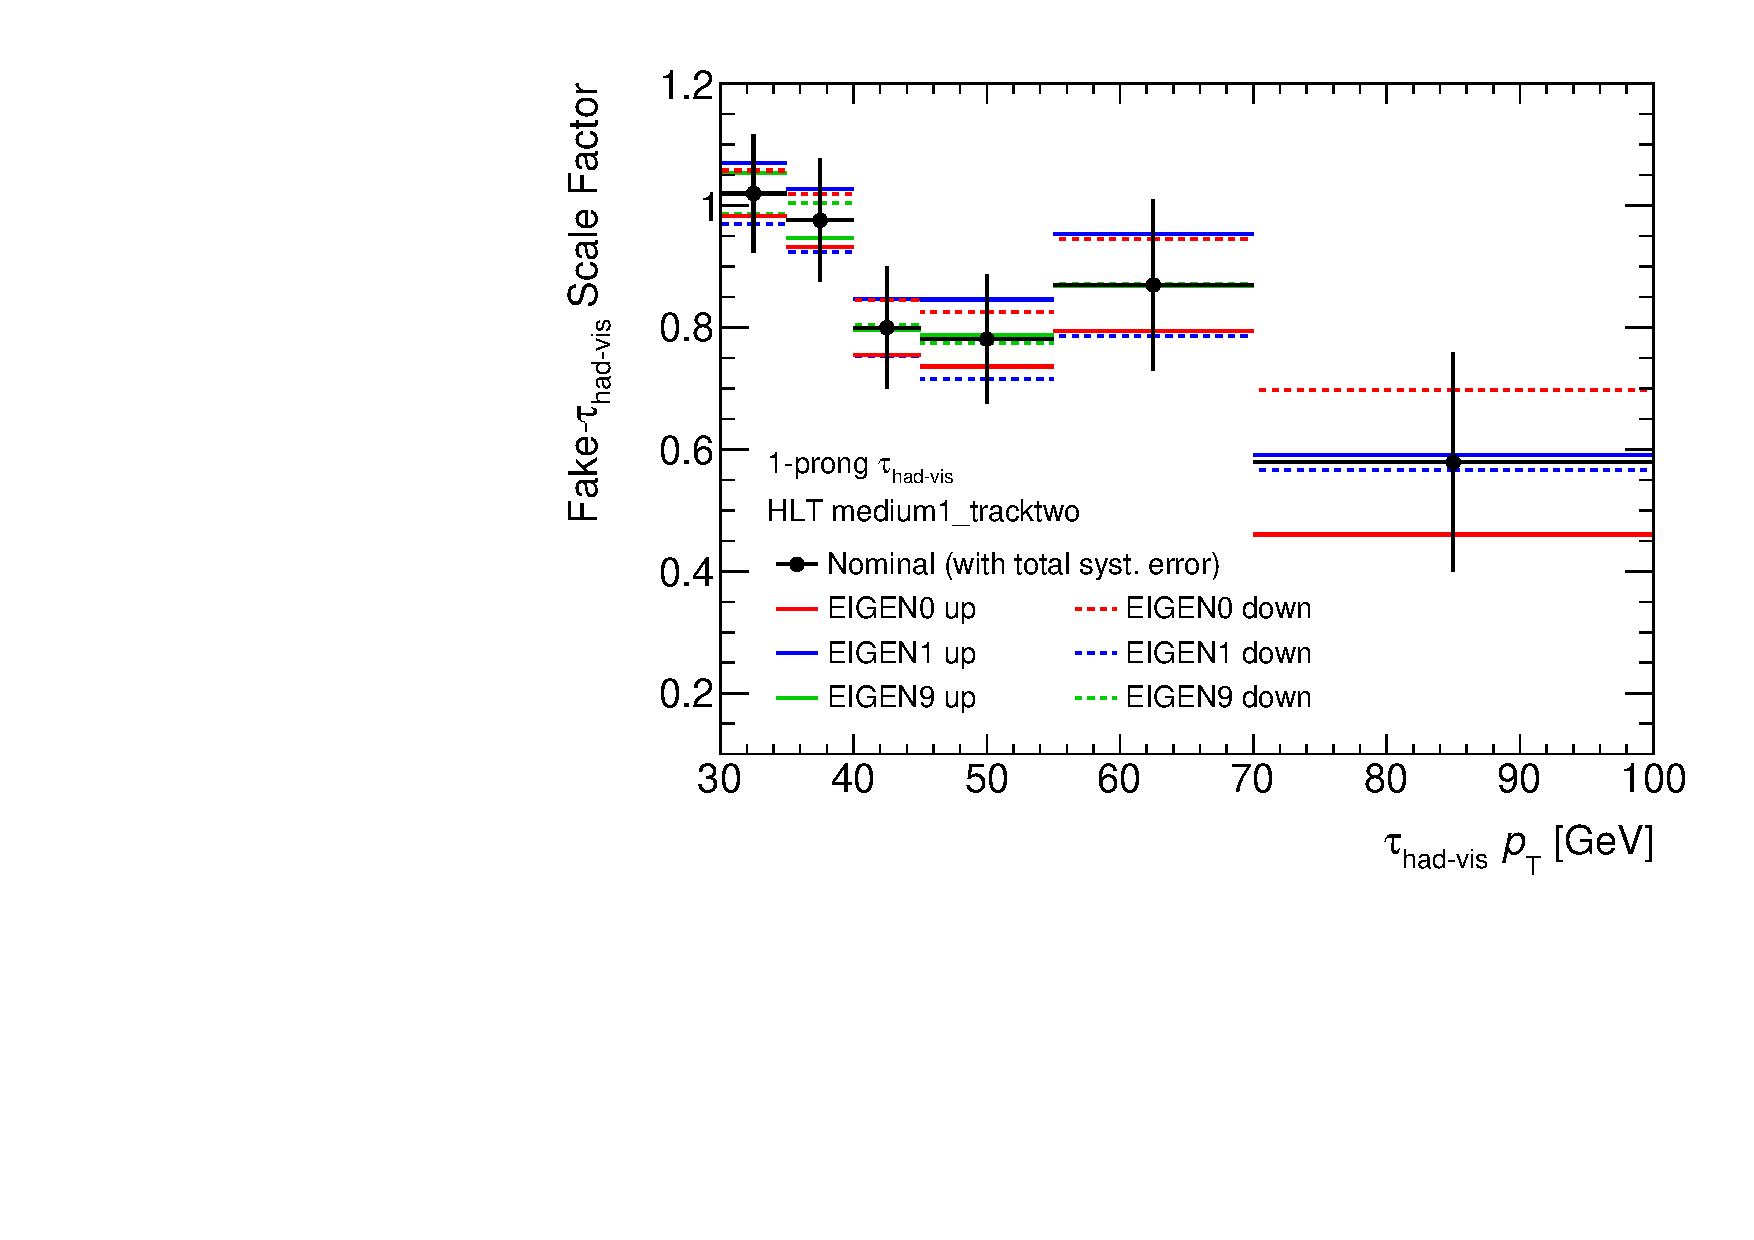
\includegraphics[width=\textwidth]{ttbarSF/ttbarSF_eigvar_1p}
    \caption{1-prong \tauhadvis}
    \label{fig:ttbarSF_eigenvariations_1p}
  \end{subfigure}\hfill%
  \begin{subfigure}[t]{.495\textwidth}
    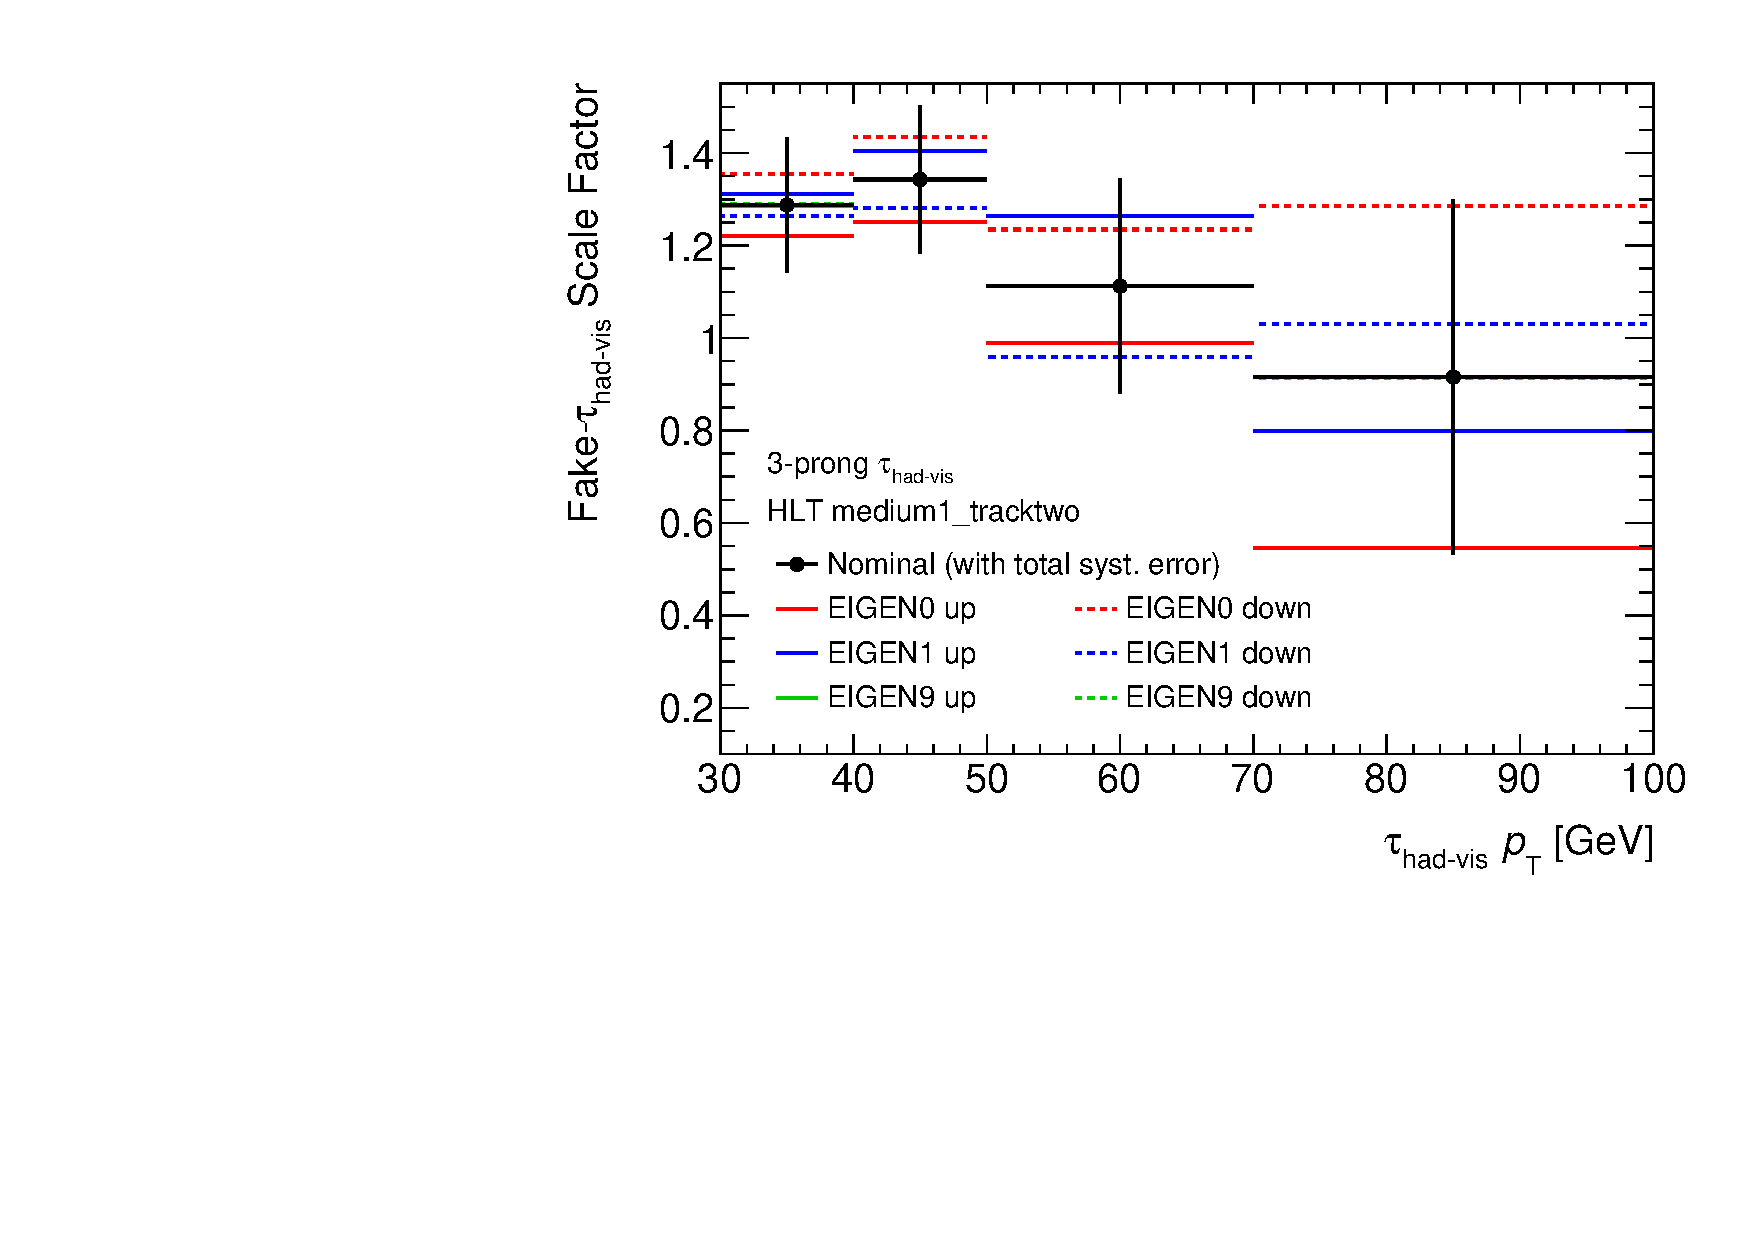
\includegraphics[width=\textwidth]{ttbarSF/ttbarSF_eigvar_3p}
    \caption{3-prong \tauhadvis}
    \label{fig:ttbarSF_eigenvariations_3p}
  \end{subfigure}

  \caption{Variations resulting from the decorrelation procedure
    applied to the \faketauhadvis scale factor measurement for the
    \texttt{HLT\_tau25\_medium1\_tracktwo} trigger. Two variations
    explaining most of the variance (\texttt{EIGEN0/1}) and the
    variation explaining least of the variance of the measurement
    (\texttt{EIGEN9}) are shown. Adding the deviations of all
    variations from the nominal result in quadrature recovers the
    total systematic error.}%
  \label{fig:ttbarSF_eigenvariations}
\end{figure}


\subsubsection{Application of \faketauhadvis Scale Factors in the
  \hadhad Channel}

The \ttbarFakes background in the signal region of the \hadhad channel
is estimated by applying \faketauhadvis scale factors to \ttbar events
from simulation with at least one \faketauhadvis. These events are
required to pass the signal region selection criteria of the \hadhad
channel, including events being selected by a trigger according to the
selection strategy described in~\Cref{sec:trigger} and reconstructed
\tauhadvis candidates being matched to \tauhadvis at the HLT.

The scale factors are chosen depending on the trigger category (STT or
DTT) and whether the \faketauhadvis is the \tauhadvis candidate
leading in \pT, sub-leading in \pT, or whether both selected
candidates are \faketauhadvis. When both \tauhadvis candidates are
originating from quark- or gluon-initiated jets, the scale factor correction is
assumed to factorise and the product of scale factors is assigned as
an event-level weight.

In events selected by di-\tauhadvis triggers, both \tauhadvis
candidates have to fulfil the trigger-level isolation and
identification requirements. In this case, the set of scale factors is
chosen according to the trigger chain that selected the event,
independently of which candidate is a \faketauhadvis. In contrast,
only one \tauhadvis candidate has to fulfil the trigger-level
requirements in the single-\tauhadvis trigger category. A
simplification is made assuming that the \tauhadvis candidate leading
in \pT satisfies the trigger conditions, causing the event to be
selected. This assumption is valid for more than \SI{99}{\percent}
\ttbar events containing \faketauhadvis in the STT
category. Therefore, scale factors measured for \faketauhadvis after
trigger-matching are applied when the leading \tauhadvis is faked by a
jet; scale factors derived without trigger-matching are applied when
the sub-leading \tauhadvis is faked by a jet. Similar to the DTT case,
if the \faketauhadvis is the \tauhadvis candidate leading in \pT then
the set of scale factors is used that corresponds to the trigger chain
that selected the event. The calculation of the multiplicative event
weight for \ttbarFakes events from simulation is summarised
in~\Cref{tab:ttbarSF_application_rule}.

\begin{table}[htbp]
  \centering

  \caption{Multiplicative event weights for the data-driven correction
    of \ttbar with \faketauhadvis from simulation. Events are
    distinguished by whether the leading \tauhadvis candidate
    ($\tau_{\text{lead}}$), the sub-leading \tauhadvis candidate
    ($\tau_{\text{subl}}$), or both are faked by a quark- or
    gluon-jet. Scale factors for \faketauhadvis without trigger
    requirements are denoted as $\text{SF}_{\text{loose}}$; scale
    factors with isolation and identification requirements at
    trigger-level by $\text{SF}_\text{loose+trig.}$.}%
  \label{tab:ttbarSF_application_rule}

  \resizebox{\textwidth}{!}{
    \begin{tabular}{cc@{\hskip 2em}rcl@{\hskip 2em}rcl}
  \toprule
  $\tau_{\text{lead.}}$ & $\tau_{\text{subl.}}$ & \multicolumn{3}{c}{Event weight (STT)} & \multicolumn{3}{c}{Event weight (DTT)} \\
  \midrule
  true & fake & $1$ & $\times$ & $\text{SF}_\text{loose}(\tau_{\text{subl.}})$
              & $1$ & $\times$ & $\text{SF}_\text{loose+trig.}(\tau_{\text{subl.}})$ \\[0.2em]

  fake & true & $\text{SF}_\text{loose+trig.}(\tau_{\text{lead.}})$ & $\times$ & $1$
              & $\text{SF}_\text{loose+trig.}(\tau_{\text{lead.}})$ & $\times$ & $1$ \\[0.2em]

  fake & fake & $\text{SF}_\text{loose+trig.}(\tau_{\text{lead.}})$ & $\times$ & $\text{SF}_\text{loose}(\tau_{\text{subl.}})$
              & $\text{SF}_\text{loose+trig.}(\tau_{\text{lead.}})$ & $\times$ & $\text{SF}_\text{loose+trig.}(\tau_{\text{subl.}})$ \\
  \bottomrule
\end{tabular}

%%% Local Variables:
%%% mode: latex
%%% TeX-master: "../phd_thesis"
%%% End:

  }
\end{table}

% When applying the scale factors to events in the 𝜏 had 𝜏 had -channel,
% an approach similar to the application of true 𝜏 had calibrations
% (e.g. trigger and offline 𝜏 had ), where it is assumed that the
% calibrations factorize in a multi-𝜏 had final state, is taken. In this
% analysis this assumption only affects the 𝑡 𝑡 ¯ final state with two
% fake 𝜏 had (FF events). This contribution is a sub-leading source of
% fake 𝜏 had making up only 15 % of the
% total 𝑡 𝑡 ¯ +fake 𝜏 had contribution (the dominant contributions are
% events where only one 𝜏 had is fake – i.e.  TF and FT events). The
% uncertainties related to the fake scale factor measurement are assumed
% to be
% fully correlated between both 𝜏 had in DTT FF events 12 and are
% propagated as such to the final background estimate in the 𝜏 had 𝜏 had
% -channel. Compared to the size of the uncertainties affecting FF
% events (e.g. 40 %
% for the 𝜏 lep 𝜏 had → 𝜏 had 𝜏 had extrapolation uncertainties,
% c.f. Table 24), deviations from this assumption are thought to be
% negligible.


\subsubsection{Systematic Uncertainties}

% \todo[inline]{How does STT play into this? The momentum thresholds are
%   unrealistically high so that it can barely be measured with this
%   approach.}

In addition to the measurement-based uncertainties, two other sources
of uncertainties are considered. These target the effect of thresholds
applied to \tauhadvis at the HLT and L1 trigger, and the extrapolation
of the scale factors from $\ell + \tauhad$ to \hadhad final states.

A systematic uncertainty on the scale factors is derived for the
effect of different \tauhadvis transverse momentum (energy) thresholds
at the HLT (L1 trigger). Events selected by di-\tauhadvis triggers
require \tauhadvis candidates to pass thresholds on the transverse
momentum (energy) of \SI{35}{\GeV} and \SI{25}{\GeV} at the HLT
(\SI{20}{\GeV} and \SI{12}{\GeV} at the L1 trigger) for the leading
and sub-leading \tauhadvis candidate, respectively. When estimating
the \ttbarFakes background where the \faketauhadvis is required to
pass trigger-matching, scale factors measured for single-\tauhadvis
triggers with thresholds of $\pTHLT > \SI{25}{\GeV}$ and
$E_{\text{T}}^{\text{L1}} > \SI{12}{\GeV}$ are applied, primarily
targeting the effect of isolation and identification requirements and
neglecting differences due to the \pT- and \ET-thresholds at
trigger-level. This is an approximation for cases where the leading
\tauhadvis candidate is mimicked by a quark- or gluon-jet, the
approximation being motivated by the large overlap in events selected
by both the lower and higher threshold trigger beyond the
$\pT > \SI{40}{\GeV}$ cut applied to the leading \tauhadvis candidate
during offline event selection.

The overlap is studied in simulated \ttbar with at least one
\faketauhadvis in the SF-CR by examining the fraction of \tauhadvis
candidates passing the $\pTHLT > \SI{35}{\GeV}$~trigger given they
pass the $\pTHLT > \SI{25}{\GeV}$~trigger. For \faketauhadvis with
$\pT > \SI{40}{\GeV}$ the overlap between triggers is
\SI{95}{\percent} for \faketauhadvis reconstructed as 1-prong
candidates; \SI{85}{\percent} for \faketauhadvis reconstructed as
3-prong candidates. %
% The difference between 1- and 3-prong candidates is caused by a
% slower increase in trigger efficiency with increasing \tauhadvis \pT
% for 3-prong candidates~\cite{ATLAS-CONF-2017-061}.
Both triggers reach near \SI{100}{\percent} overlap for 1-prong
candidates with $\pT > \SI{50}{\GeV}$ and 3-prong candidates with
$\pT > \SI{60}{\GeV}$.\todo{Plot?} No uncertainty is introduced for
larger transverse momenta due to negligible differences between both
triggers.

The scale factor measurement is repeated for the single-\tauhadvis
triggers with higher thresholds and compared to the nominal result in
the \faketauhadvis \pT region from \SI{40}{\GeV} up to \SI{50}{\GeV}
or \SI{60}{\GeV} for 1- and 3-prong candidates, respectively. The
scale factors measured for the higher threshold triggers agree within
\SI{10}{\percent} with the nominal result. The deviation from the
nominal measurement is assigned as an additional uncertainty when the
leading \tauhadvis candidate originates from a quark- or
gluon-jet. The size of the uncertainties are summarised
in~\Cref{tab:ttbarSF_tau25_35_uncertainty}. These uncertainties have a
sub-percent impact on the overall normalisation of the \ttbarFakes
background with the \pT-leading \tauhadvis candidate being a
\faketauhadvis in the \hadhad signal region. This is due the
transverse momentum of the leading \tauhadvis typically exceeding the
trigger threshold with a sufficiently large margin such that the
uncertainties do not apply. This source of uncertainty is small
compared to uncertainties from the scale factor measurement, however,
it is still considered for later statistical analysis.

\begin{table}[htbp]
  \centering

  \caption{Size of the uncertainty comparing scale factors measured
    for triggers with $\pTHLT > \SI{25}{\GeV}$ and
    $\pTHLT > \SI{35}{\GeV}$ thresholds. The uncertainty is given
    relative to all events from \ttbar in the \hadhad channel signal
    region where the leading \tauhadvis is a \faketauhadvis with \pT
    close to the \SI{40}{\GeV} threshold.}%
  \label{tab:ttbarSF_tau25_35_uncertainty}

  \begin{tabular}{lcc}
  \toprule
  & {1-prong \tauhadvis} & {3-prong \tauhadvis} \\
  & {(40 - 50 GeV)} & {(40 - 60 GeV)} \\
  \midrule
  \texttt{medium1\_tracktwo} (ttbarFT) & $\pm 5.8 \%$ & $\pm 5.5 \%$ \\
  \texttt{medium1\_tracktwo} (ttbarFF) & $\pm 5.9 \%$ & $\pm 5.2 \%$ \\[0.5em]

  \texttt{medium1\_tracktwoEF} (ttbarFT) & $\pm 6.4 \%$ & $\pm 8.1 \%$ \\
  \texttt{medium1\_tracktwoEF} (ttbarFF) & $\pm 6.4 \%$ & $\pm 8.0 \%$ \\[0.5em]

  \texttt{mediumRNN\_tracktwoMVA} (or EF) (ttbarFT) & $\pm 3.8 \%$ & $\pm 2.7 \%$ \\
  \texttt{mediumRNN\_tracktwoMVA} (or EF) (ttbarFF)& $\pm 4.0 \%$ & $\pm 2.6 \%$ \\
  \bottomrule
\end{tabular}

%%% Local Variables:
%%% mode: latex
%%% TeX-master: "../phd_thesis"
%%% End:

\end{table}

The measurement of the scale factors is performed in a region
($\ell+\tauhad$ SF-CR) different from where they are applied (\hadhad
SR). An uncertainty is assigned on the relative difference in the
acceptance of \ttbarFakes between the measurement region and the
application region, effectively serving as an extrapolation
uncertainty. This uncertainty is determined by performing variations
of the \ttbar modelling in simulation and estimating the change in
relative acceptance between both regions, the relative acceptance
being the ratio of the acceptance in the application region and the
measurement region.

The estimation of extrapolation uncertainties between SF-CR and
\hadhad SR considers the same sources of \ttbar modelling variations
as used for the scale factor measurement. Different parameterisation
are derived for \ttbar with a single \faketauhadvis and two
\faketauhadvis in the \hadhad SR.

For \ttbar events with a single \faketauhadvis in the \hadhad SR the
extrapolation uncertainty is examined in dependence on \pT of the
\faketauhadvis, separately for 1- and 3-prong candidates. Except for
the parton shower variation, no \tauhadvis \pT-dependent effect of the
uncertainty is observed.  The comparison of alternative parton shower
programs, comparing \PYTHIA[8] and \HERWIG[7], results in a
shape-dependence of the extrapolation uncertainty as a function of
\tauhadvis \pT which is shown in~\Cref{fig:ttbarSF_extrapol_shape}.
Similar to the modelling uncertainties for the measurement, a
polynomial is fitted to smoothly interpolate the uncertainty over a
range of \tauhadvis \pT. %\todo{Interpretation. What if pT > 150?}

\begin{figure}[htbp]
  \centering

  \begin{subfigure}[t]{.495\textwidth}
    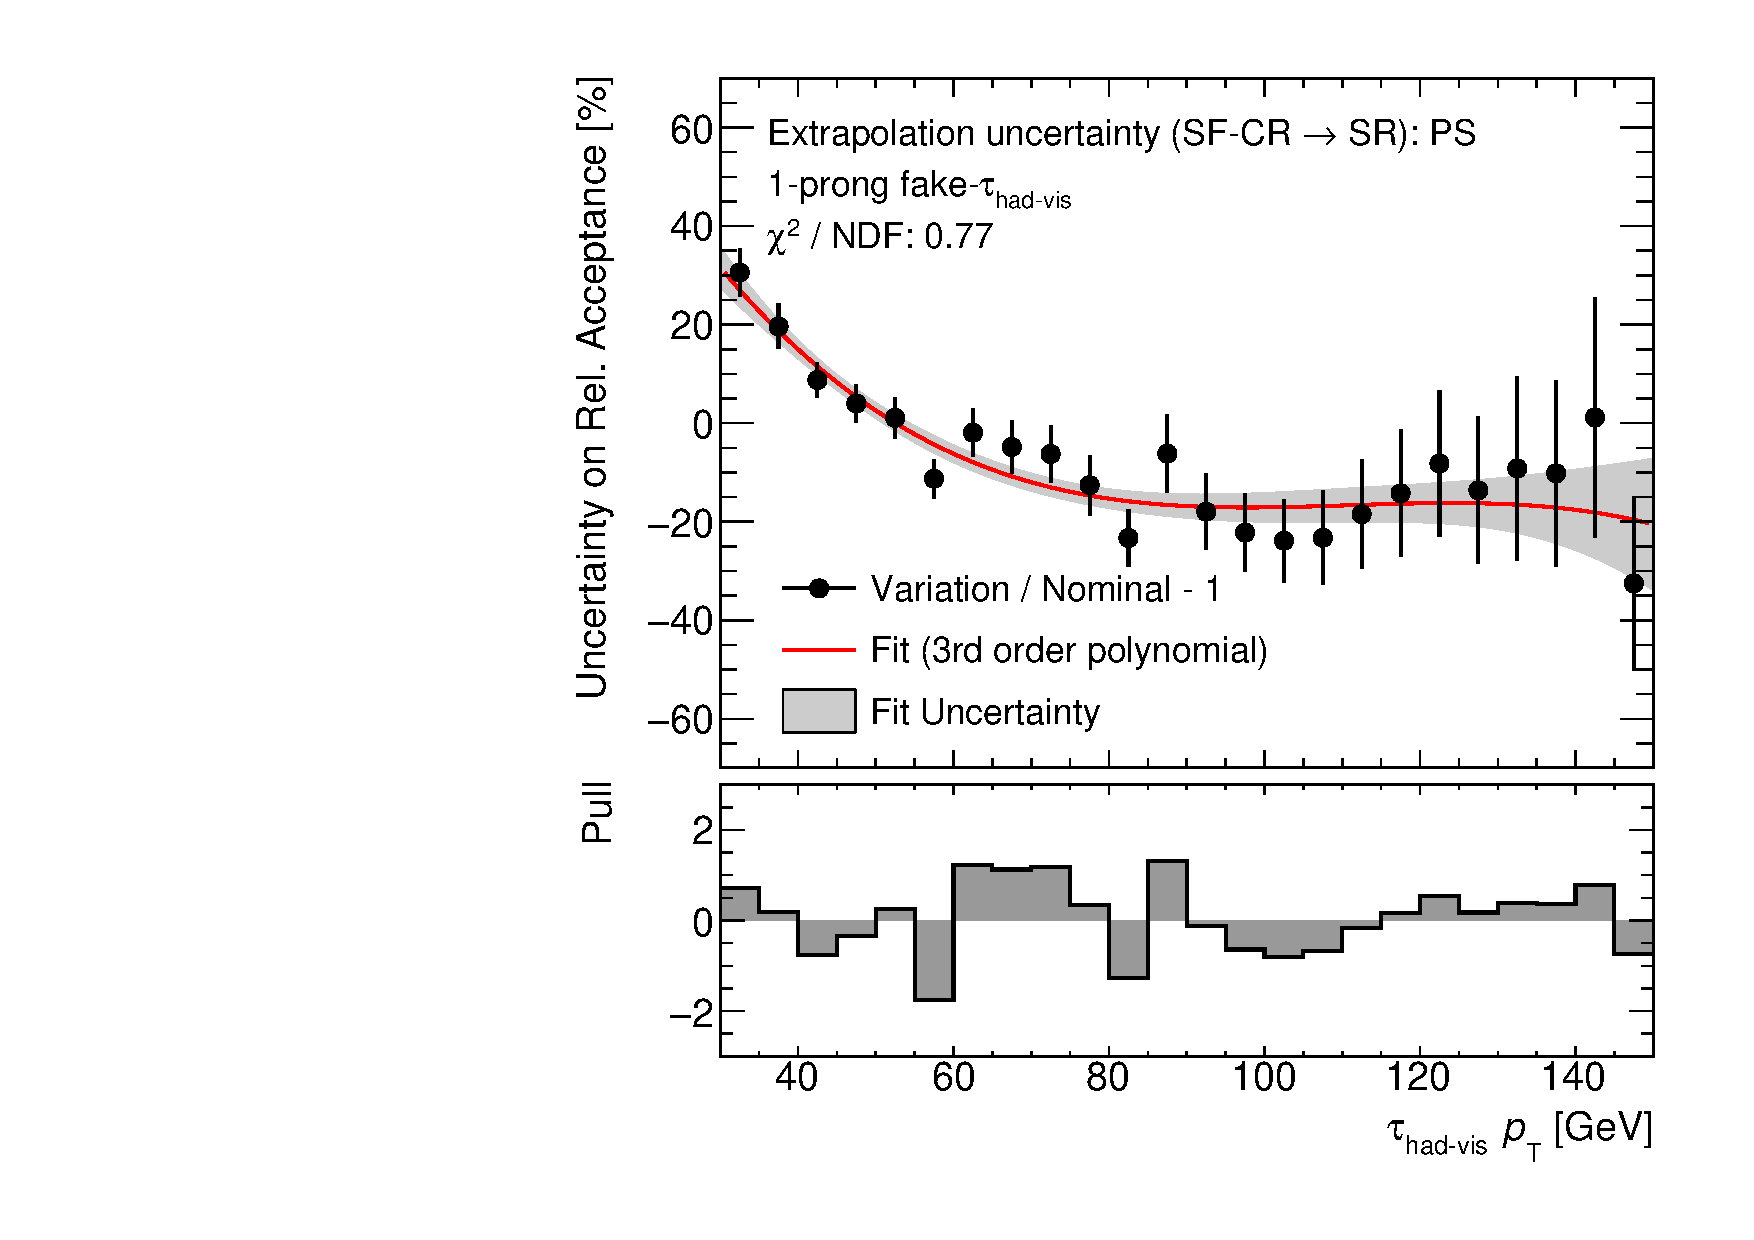
\includegraphics[width=\textwidth]{ttbarSF/ttbarSF_extrapol_PS_1p}
    \caption{}
    \label{fig:ttbarSF_extrapol_shape_a}
  \end{subfigure}\hfill%
  \begin{subfigure}[t]{.495\textwidth}
    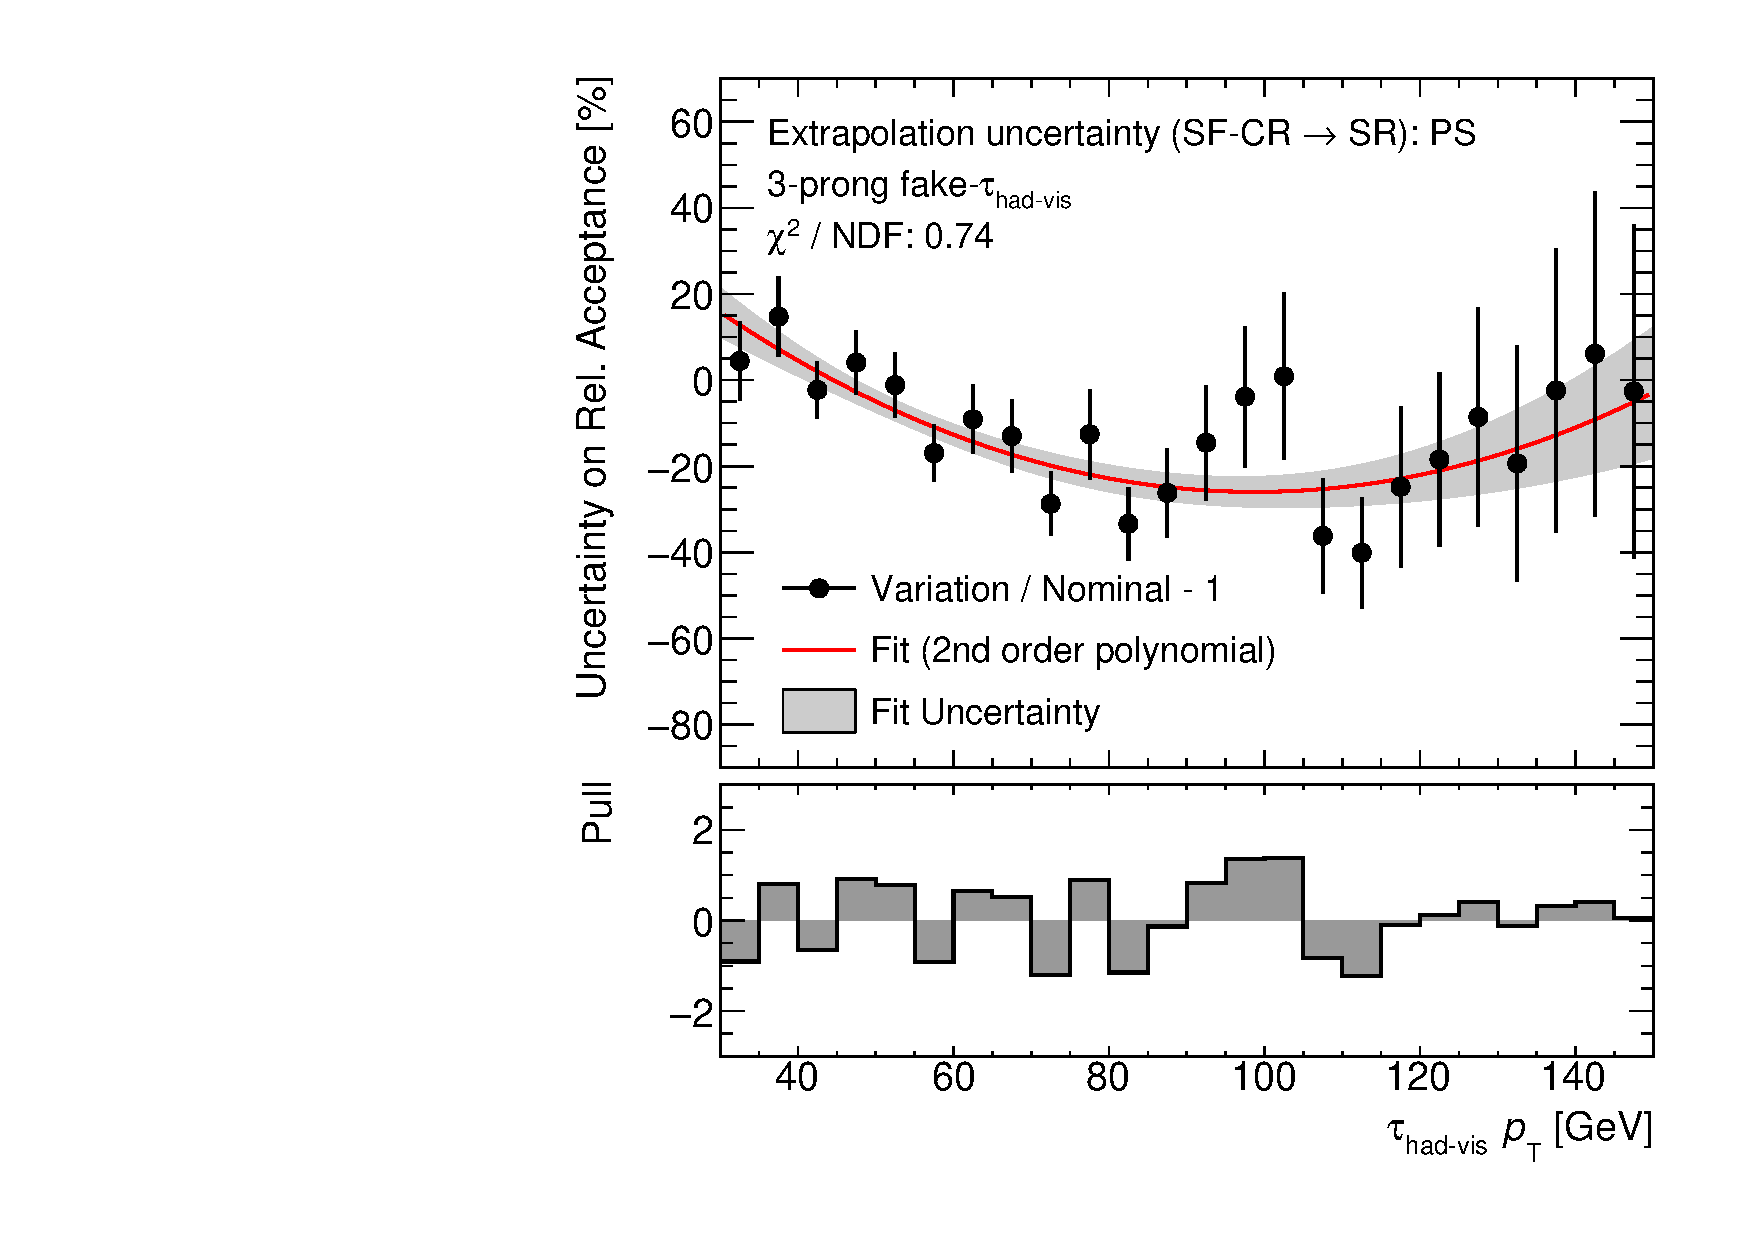
\includegraphics[width=\textwidth]{ttbarSF/ttbarSF_extrapol_PS_3p}
    \caption{}
    \label{fig:ttbarSF_extrapol_shape_b}
  \end{subfigure}

  \caption{Extrapolation uncertainty of the scale factors measured in
    the SF-CR to the \hadhad SR based on parton shower comparisons
    (\PYTHIA[8] and \HERWIG[7]). The uncertainty is shown for 1-prong
    (a) and 3-prong \faketauhadvis (b) including a fit of polynomials
    to the binned estimate of the uncertainty.}
  \label{fig:ttbarSF_extrapol_shape}
\end{figure}

A different approach is taken for the extrapolation uncertainty
between SF-CR and \hadhad SR for cases where both \tauhadvis
candidates are faked by a quark- or gluon-jet. Only a normalisation
uncertainty is assigned due to the ambiguous matching of \tauhadvis
candidates between the \lephad (one \faketauhadvis) and the \hadhad
region (two \faketauhadvis). This approximation is made to avoid this
ambiguity and is further motivated by events with two \faketauhadvis
being a subdominant contribution to the total \ttbarFakes background.

The extrapolation uncertainties are summarised
in~\Cref{tab:ttbarSF_acceptance_uncertainty}. The parton shower
variations dominate the total uncertainty on the relative acceptance
between the SF-CR and the SR, ranging from \SIrange{20}{40}{\percent}.

\begin{table}[htbp]
  \centering

  \caption{Normalisation uncertainties on the relative acceptance
    between SF-CR and SR. The uncertainties are symmetrised and
    rounded to two significant figures. $\dagger$: The parton shower
    uncertainty is parameterised as a function of \tauhadvis \pT (see
    also~\Cref{fig:ttbarSF_extrapol_shape}) and is not included in the
    total uncertainty.}%
  \label{tab:ttbarSF_acceptance_uncertainty}

  \begin{tabular}{l
  S[table-format=1.3]
  S[table-format=1.2]
  S}
  \toprule
  Source & {Uncertainty (1-prong) / \%} & {Uncertainty (3-prong) / \%} & {Uncertainty (FF) / \%} \\
  \midrule
  ME & 1.7 & 6.0 & 9.2 \\
  PS & {--$^\dagger$} & {--$^\dagger$} & 35 \\
  \hdamp & 1.6 & 8.2 & 4.6 \\
  \muF & 0.18 & 0.22 & \\
  \muR & 0.040 & 0.50 & \\
  ISR & 0.22 & 0.68 & \\
  FSR & 4.0 & 8.5 & \\
  \midrule
  Total & 4.7 & 14 & \\
  \bottomrule
\end{tabular}

%%% Local Variables:
%%% mode: latex
%%% TeX-master: "../phd_thesis"
%%% End:

\end{table}


\subsubsection{Discussion}

The determination of the \ttbarFakes background in the \hadhad signal
region using the scale factor method described in this section
provides a way to estimate this background and its uncertainty based
on a measurement-driven approach. In~\Cref{tab:ttbarSF_yields} the
event yield of \ttbarFakes in the \hadhad signal region is shown and
compared to \ttbar simulation without corrections.

\begin{table}[htbp]
  \centering

  \caption{Total event yield in simulated \ttbar with \faketauhadvis
    in the \hadhad SR before and after correction using the measured
    scale factors. The uncorrected event yield is shown with MC
    statistical uncertainties only; the corrected event yield with MC
    statistical and systematic uncertainties of the scale factor
    method. The \ttbarFakes background is partitioned into cases where
    the \pT sub-leading \tauhadvis candidate is fake (TF), the leading
    candidate is fake (FT), and both candidates are fake (FF).}%
  \label{tab:ttbarSF_yields}

  % Source:
% https://docs.google.com/spreadsheets/d/1uwVElPaR1HuqEHaL8eAh5pEoGdK2ZBQ8D_Ob8lSSPwE/edit#gid=0

% fSumw[1]=2705.09, x=0.5, error=22.9788

% Only measurement uncertainties
% ttbarSFTF: 1433.95 +- 87.88
% ttbarSFFT: 698.52 +- 72.21
% ttbarSFFF: 358.92 +- 53.50
% Total: 2491.39 +- 21.59 +- 202.99 = 204.13493

\begin{tabular}{
  l
  @{\hskip 16pt}
  S[table-format=4.0(2)]
  @{\hskip 16pt}
  S[table-format=4.0(3)]
  }
  \toprule
  & \multicolumn{2}{c}{Expected number of events (pre-fit)} \\
  \cmidrule{2-3}
          & {Simulation} & {Simulation with} \\
  Process &              & {\faketauhadvisC SF}  \\
  \midrule
  \ttbar + \faketauhadvisC (TF) & 1428 +- 16 & 1430 +- 230 \\
  \ttbar + \faketauhadvisC (FT) & 854 +- 13 & 699 +- 88 \\
  \ttbar + \faketauhadvisC (FF) & 423 +- 12 & 360 +- 160 \\
  \midrule
  \ttbar + \faketauhadvisC (total) & 2705 +- 23 & 2490 +- 320 \\
  \bottomrule
\end{tabular}

%%% Local Variables:
%%% mode: latex
%%% TeX-master: "../phd_thesis"
%%% End:

\end{table}

The total \ttbarFakes event yield in the \hadhad SR is determined with
a relative uncertainty of \SI{13}{\percent}, agreeing with the
uncorrected estimate of the total yield within uncertainties. The
expected number of \ttbarFakes events is slightly smaller after
correction since the measured scale factors for high \pT
\faketauhadvis tend to be smaller than unity. This is also reflected
in the larger relative change of the the FT-component (the leading
\tauhadvis candidate is a \faketauhadvis), for which the
\faketauhadvis has an average \pT of \SI{65}{\GeV}.

The uncertainty on the total \ttbarFakes yield in the \hadhad SR can
be separated by category to give the relative importances of different
sources of uncertainty:
\begin{align*}
  \sigma_\text{total}^{\ttbarFakes} = \valuesep\numerrt{22}{stat.}%
  \valuesep\numerrt{210}{meas.}%
  \valuesep\numerrt{240}{extrapol.}%
  \valuesep\numerrt{3.6}{trigger threshold} \,\text{.}
\end{align*}
The uncertainties originating from the SF measurement in the SF-CR
(meas.) and the extrapolation uncertainties (extrapol.) have
uncertainties of similar size. The extrapolation uncertainty is
dominated by the comparison of different parton shower programs. The
\faketauhadvis \pT-dependent PS uncertainty, affecting the TF- and
FT-components of the background, has a particularly large impact on
the TF contribution. This is due to the large uncertainty for 1-prong
\faketauhadvis candidates, making up $\frac{3}{4}$ of \faketauhadvis
in \ttbar, at low transverse momenta as shown
in~\Cref{fig:ttbarSF_extrapol_shape_a}. Due to the momentum ordering,
the average \faketauhadvis \pT in \ttbarFakes (TF) is approximately
\SI{40}{\GeV}.

Statistical uncertainties from the finite number of simulated events
(stat.) and the uncertainty based on the comparison of different
trigger thresholds (trigger threshold) have negligible impact on the
total yield in the \hadhad SR.

% Measurement uncertainties on total yield are highly correlated:
% ca. 90%
% PS uncertainty for 1-prong taus is anti-correlated due to
% sign-change of uncertainty

\todo[inline]{More comparison of fake estimates? Some validation plots?}


\subsubsection{Estimation of \faketauhadvis scale factors for the
  Anti-ID region}

The estimation of the \multijet background in the \hadhad SR, to be
described in~\Cref{sec:bkg_hadhad_ff}, requires a large subtraction of
\ttbarFakes events in the 2 $b$-tag \antiid region for \tauhadvis with
electric charge of opposite sign. The scale factor method for
estimating the \ttbarFakes background is extended to the \antiid
region to provide uncertainties on the subtraction performed as part
of the \multijet estimation.

The scale factor measurement is repeated using the same SF-CR
definition except for inverting the offline \tauhadvis identification
requirement. Instead of \tauhadvis passing loose offline \tauid,
\tauhadvis are required to fail the loose working point but exceed a
RNN \tauid score threshold of \num{0.01}. The same requirements from
the ID-region measurement regarding the reconstruction and
identification of \tauhadvis at the HLT are imposed.

The inversion of the \tauid requirement rejects most \ttbar events
with \tauhadvis originating from hadronic decays of \tauleptons,
yielding a region with high purity of \ttbarFakes
(ca.~\SI{80}{\percent}). Matching anti-\tauhadvis from the offline
reconstruction to \tauhadvis at the HLT reduces the total \ttbarFakes
yield by about \SI{80}{\percent} due to the trigger-level
identification requirements, the \ttbarFakes purity staying largely
unchanged, however.

A reduced set of experimental uncertainties is used for this
measurement due to practical limitations in the dataset preparation
for the $\ell + \tauhad$ \antiid region. Uncertainties varying the
four-momentum of reconstructed objects are omitted except
uncertainties on the \tauhadvis energy scale. Other uncertainties that
can be expressed by alternative event weights, for example
uncertainties on tagging efficiencies, are considered. Due to this
constraint, the total deviation of the central value of the scale
factors measured in the \antiid region from unity is assigned as an
additional uncertainty and propagated to the \multijet estimate in the
\hadhad SR.

The scale factors measured in the Anti-ID region are shown
in~\Cref{fig:ttbarSF_antiid_SF}. The contribution of \faketauhadvis
reconstructed as 1-prong candidates predicted by simulation agrees
well with the data-driven measurement. For 3-prong candidates,
deviations of up to \SI{20}{\percent} from simulation are observed.

\begin{figure}[htbp]
  \centering

  \begin{subfigure}[t]{.495\textwidth}
    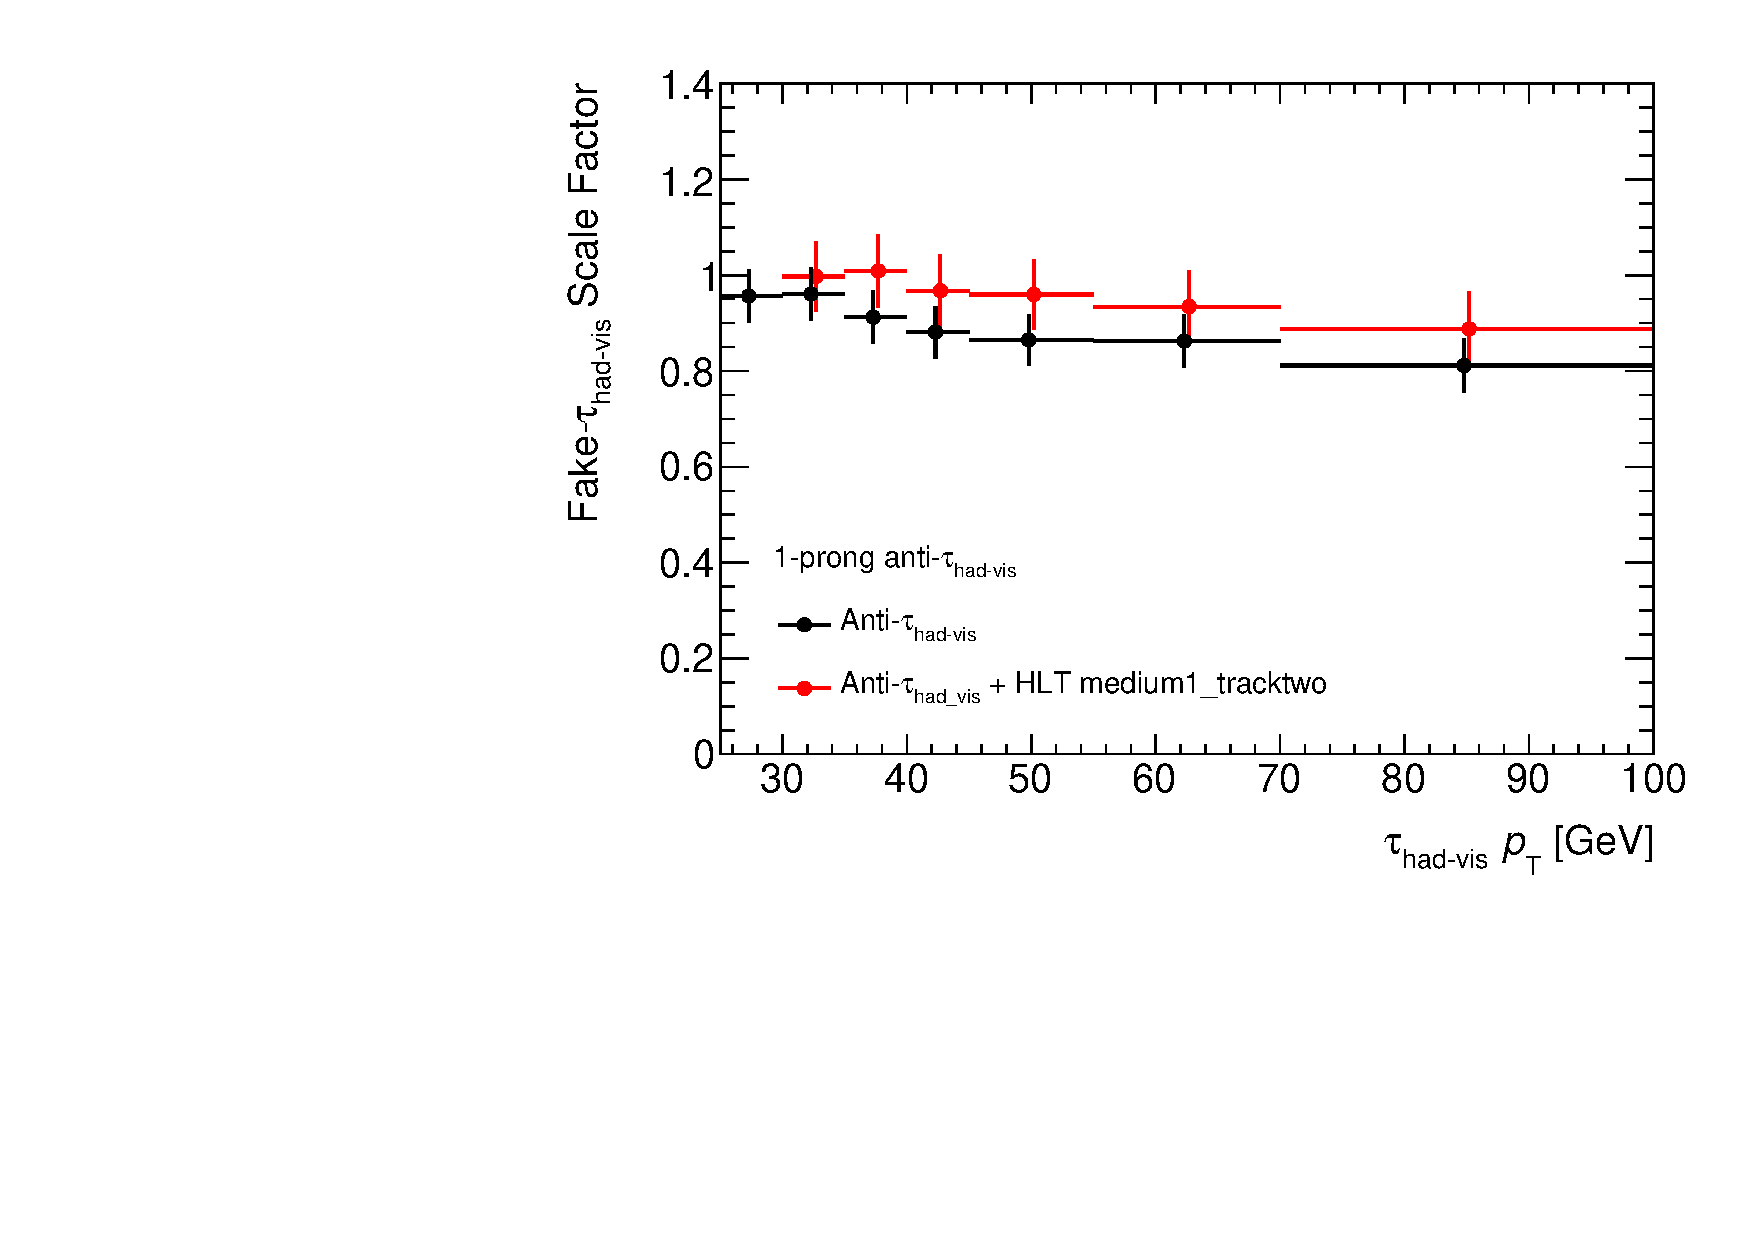
\includegraphics[width=\textwidth]{ttbarSF/scale_factors/ttbarSF_antitau_offl_tau25_1p}
    \caption{}
    \label{fig:ttbarSF_antiid_SF_a}
  \end{subfigure}\hfill%
  \begin{subfigure}[t]{.495\textwidth}
    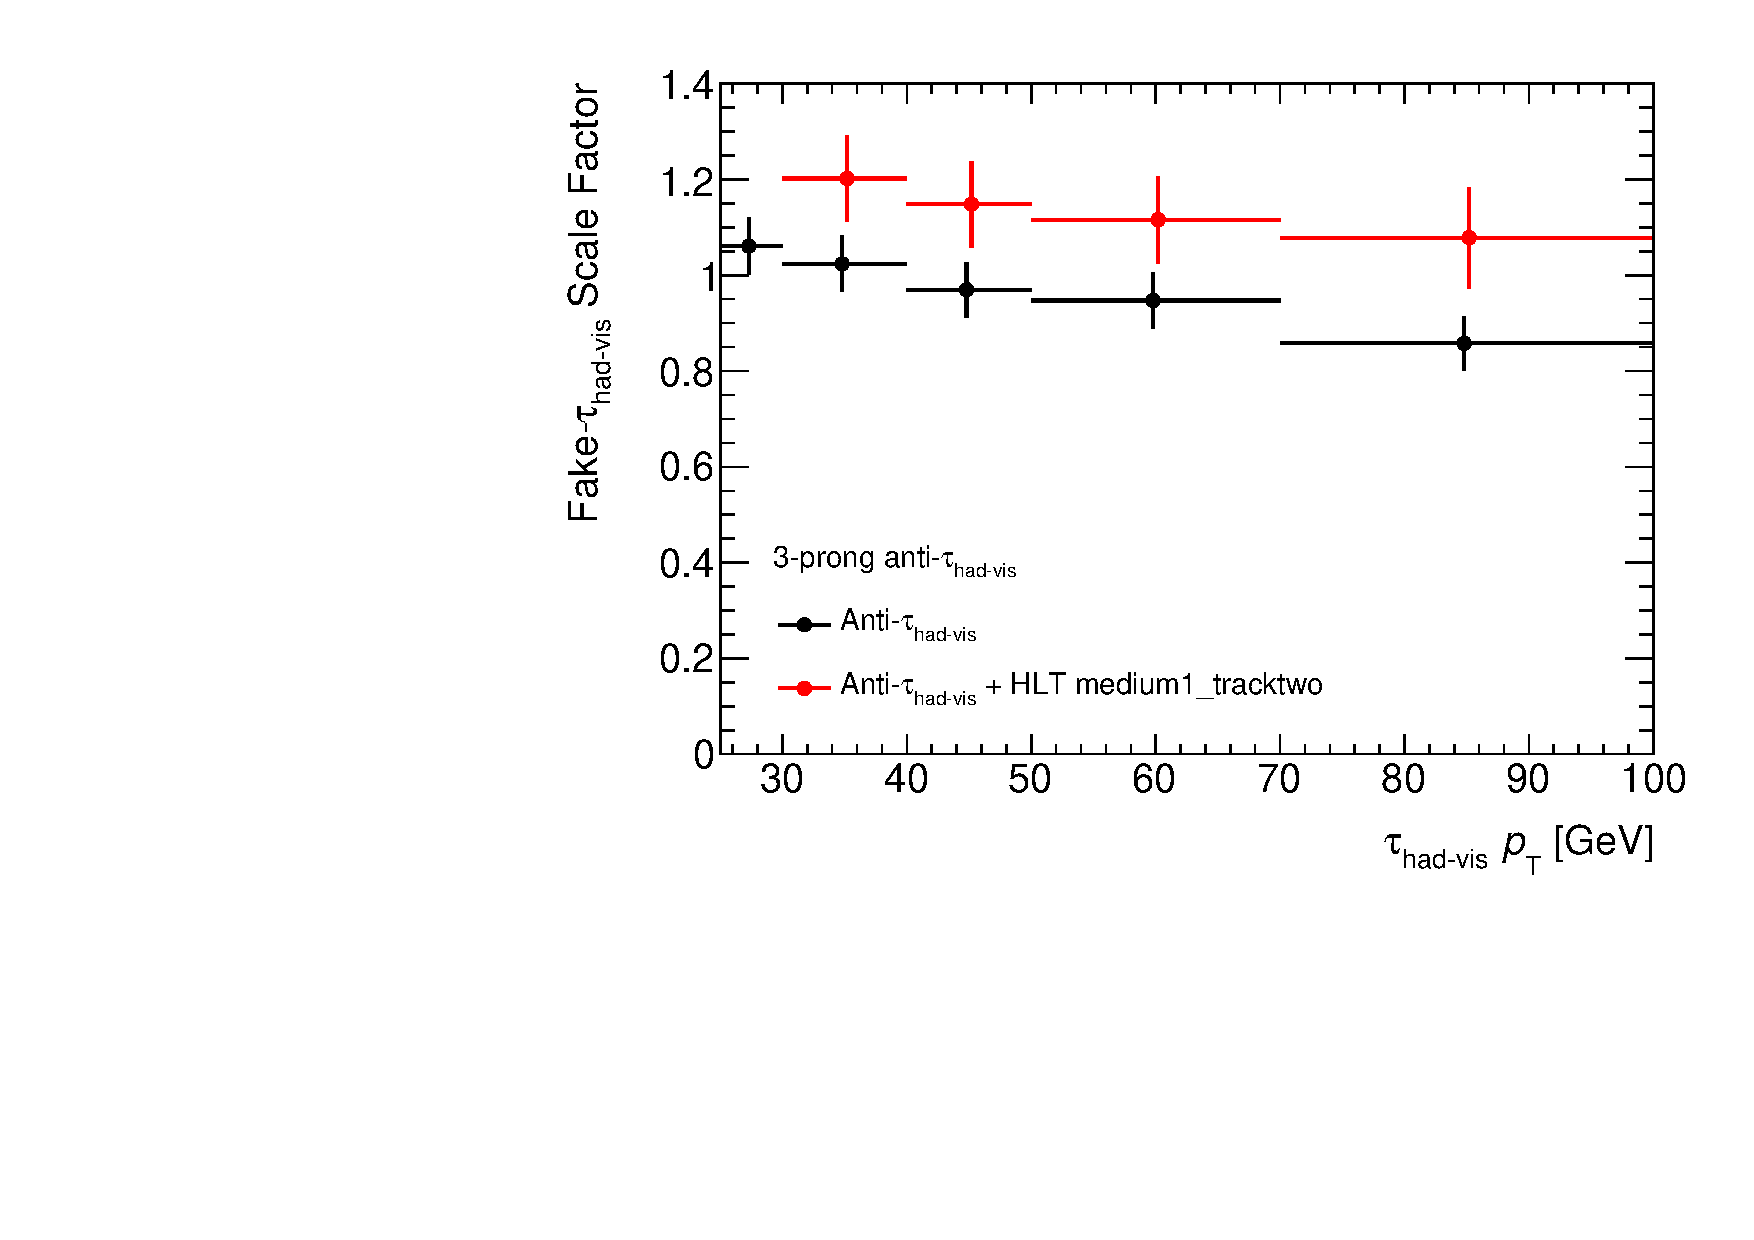
\includegraphics[width=\textwidth]{ttbarSF/scale_factors/ttbarSF_antitau_offl_tau25_3p}
    \caption{}
    \label{fig:ttbarSF_antiid_SF_b}
  \end{subfigure}

  \begin{subfigure}[t]{.495\textwidth}
    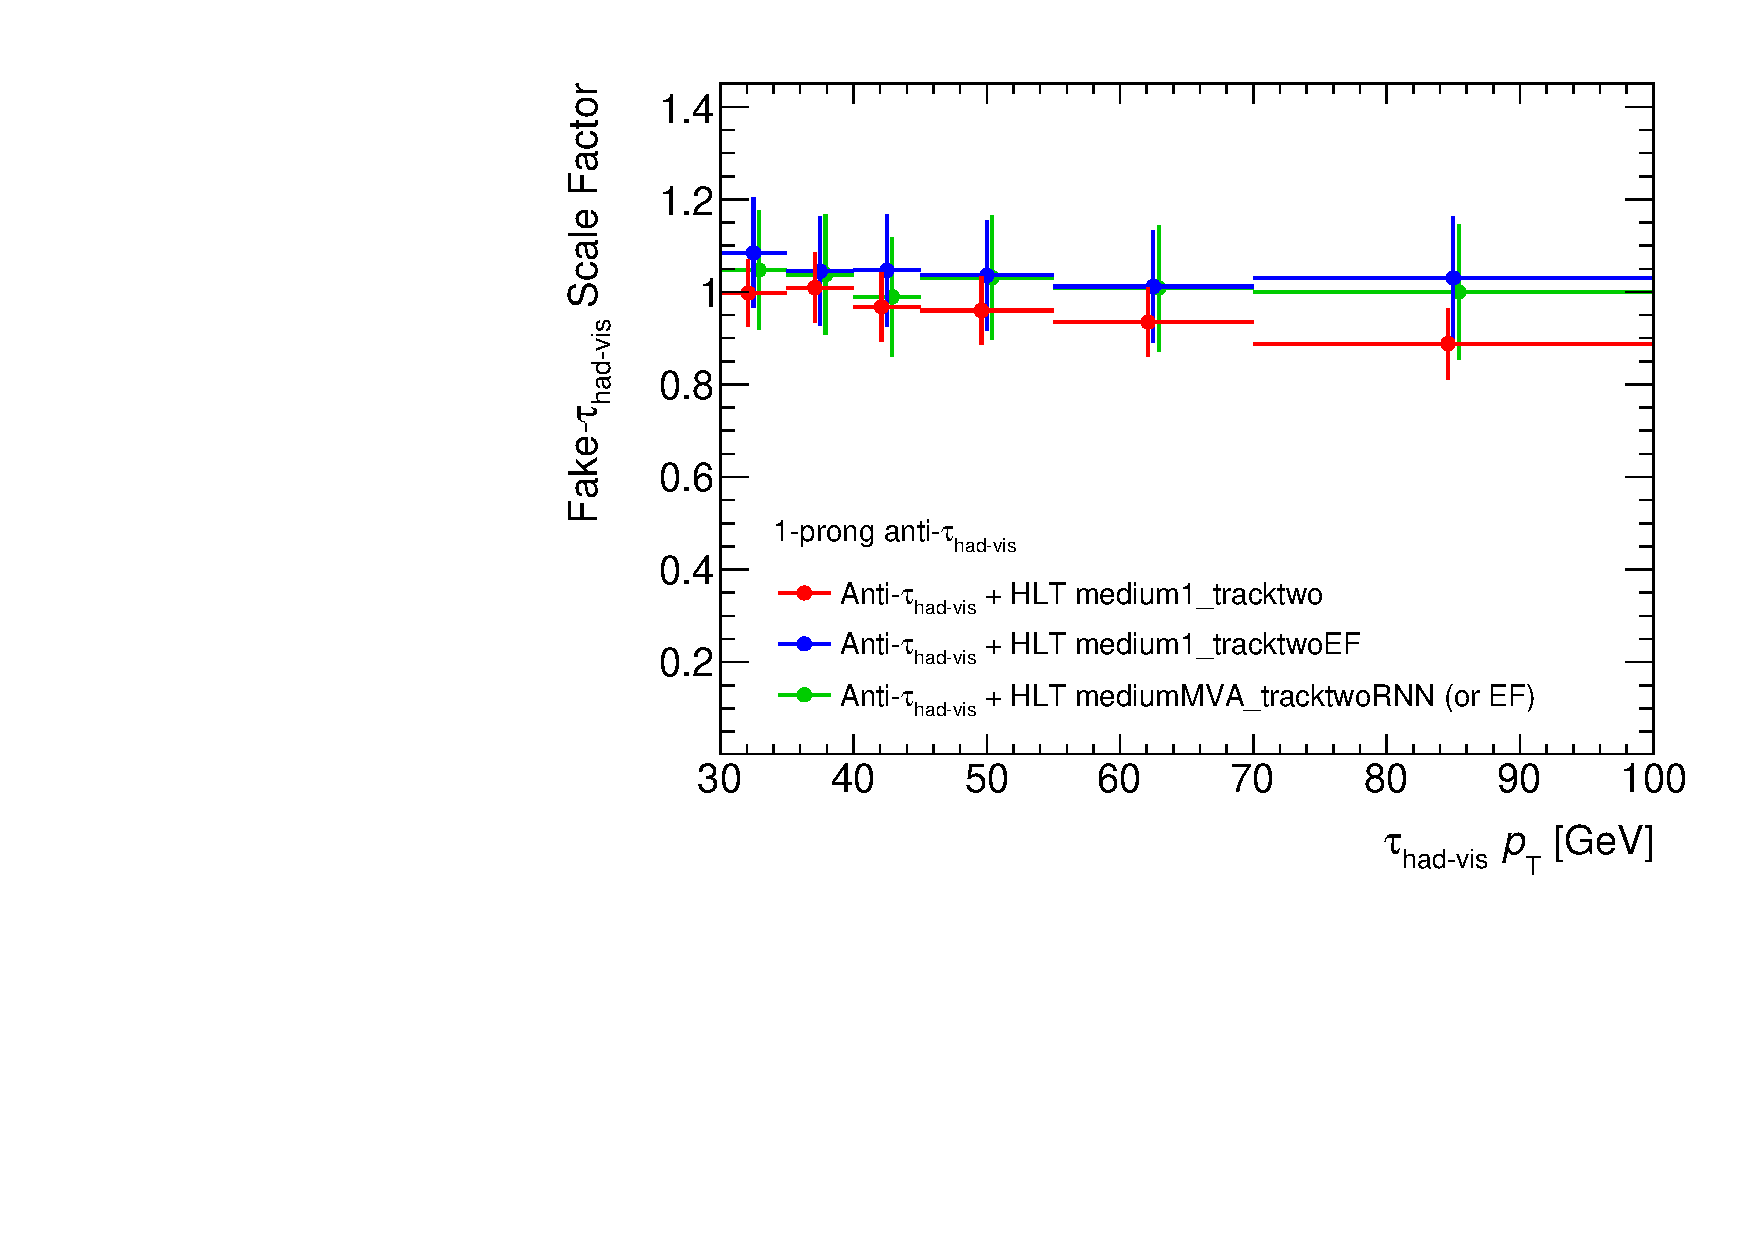
\includegraphics[width=\textwidth]{ttbarSF/scale_factors/ttbarSF_antitau_tau25_1p}
    \caption{}
    \label{fig:ttbarSF_antiid_SF_c}
  \end{subfigure}\hfill%
  \begin{subfigure}[t]{.495\textwidth}
    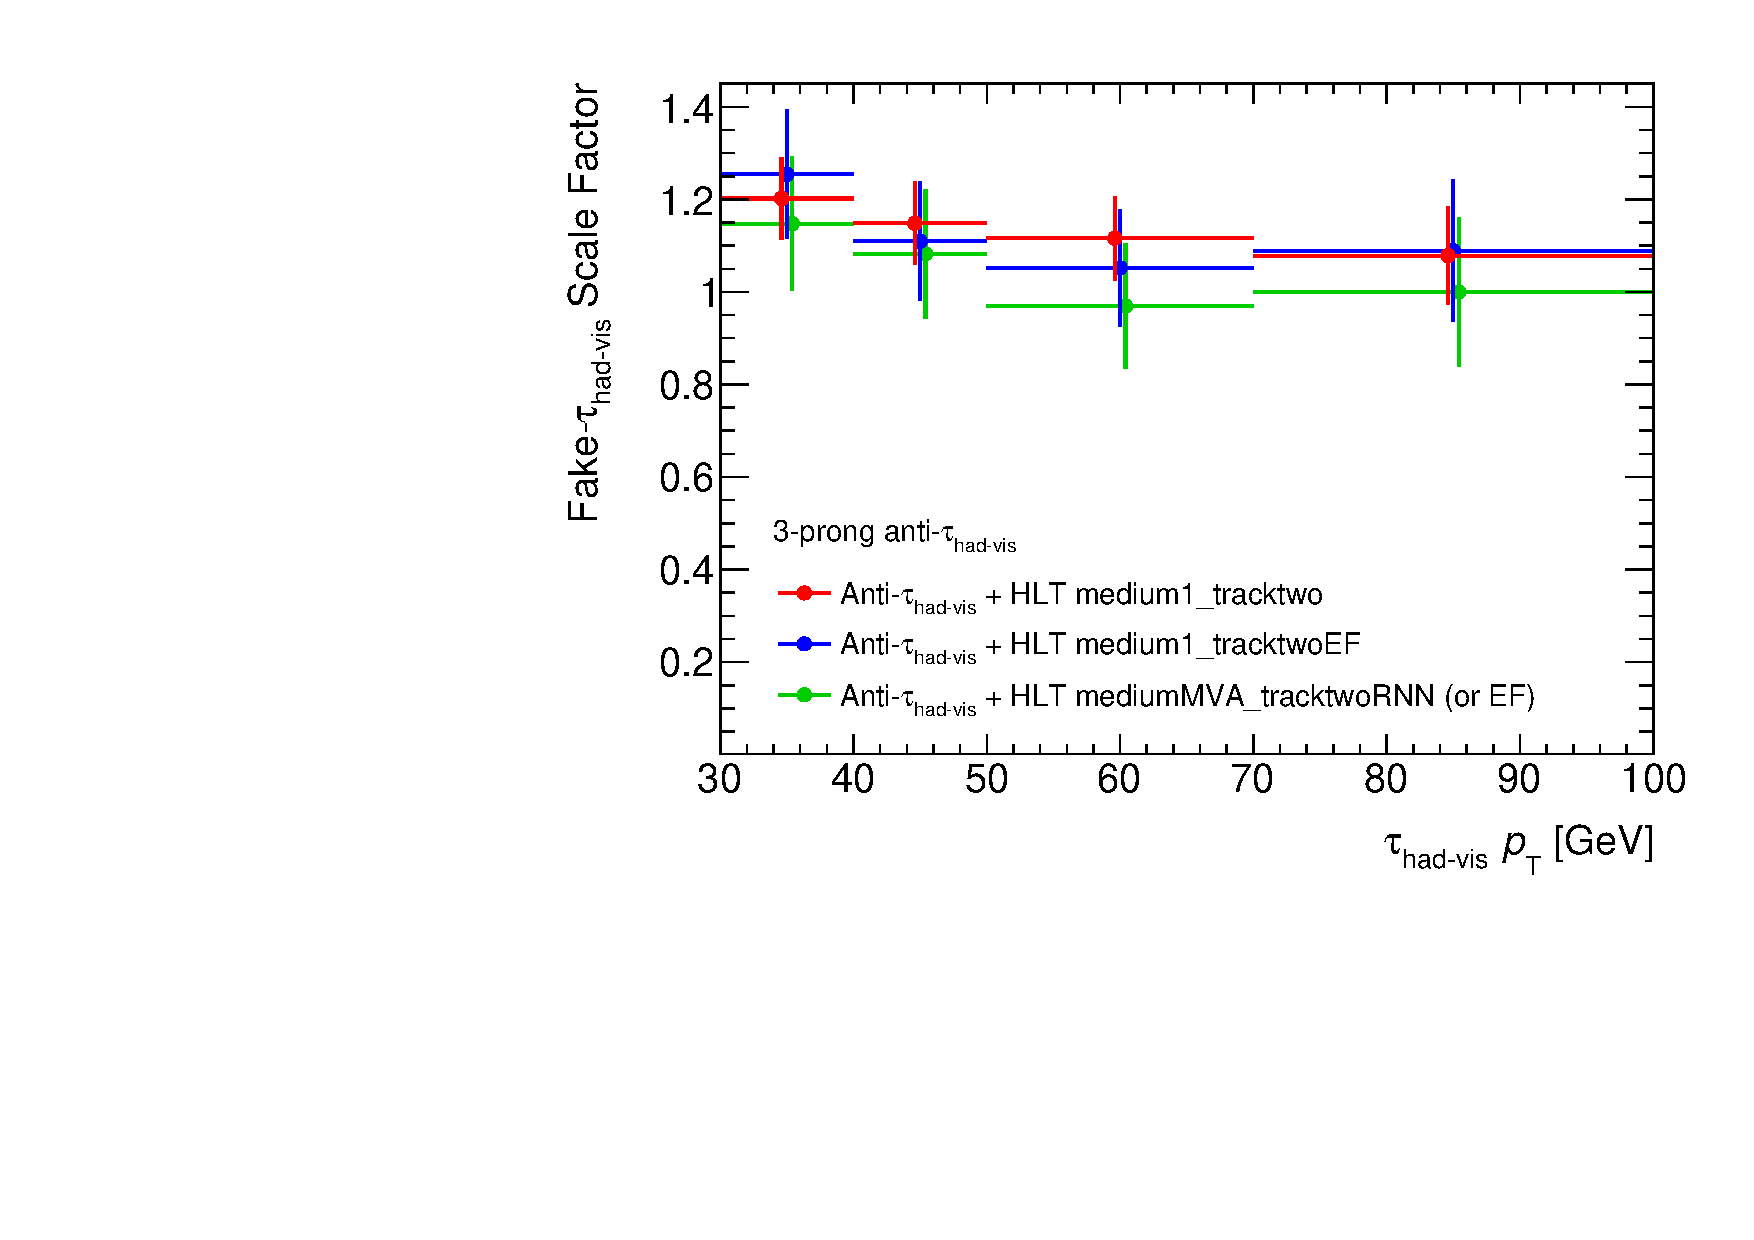
\includegraphics[width=\textwidth]{ttbarSF/scale_factors/ttbarSF_antitau_tau25_3p}
    \caption{}
    \label{fig:ttbarSF_antiid_SF_d}
  \end{subfigure}

  \caption{Scale factors for \faketauhadvis from \ttbar simulation in
    the Anti-ID region separated \tauhadvis identification criteria
    applied at trigger-level. Figures (a) and (b) compare the scale
    factors with and without \tauid at the HLT. The effect of
    different \tauhadvis trigger chains on the extracted scale factors
    is shown in (c) and (d). The last bin summarises events with
    \tauhadvis~$\pT \geq \SI{70}{\GeV}$. The markers are shifted from
    the geometrical bin centre for illustration purposes.}%
  \label{fig:ttbarSF_antiid_SF}
\end{figure}

The same decorrelation technique is used to propagate the measurement
uncertainties when applying the scale factors in the Anti-ID region of
the \hadhad channel. The rules for applying scale factors remain
unchanged with respect to the scale factor application in the
ID-region. The context and impact of the scale factors for the Anti-ID
region on the \multijet estimate will be further discussed in the
following section.

% Only the leading
% variations are used to define the subtraction uncertainty.

% \todo[inline]{Possibly include the SS region (in addition to OS) to
% get better constraints on ttbar and ttbarFakes. Possibly can float
% both true and fake \ttbar in every region reducing the correlation
% between the resulting NFs. One would have to account for possible
% biases from charge correlations.}


%%% Local Variables:
%%% mode: latex
%%% TeX-master: "../../phd_thesis"
%%% End:
